\documentclass[12pt,titlepage,letterpaper]{book}
\usepackage{titlesec}
\usepackage{anysize}
\usepackage{graphicx}
\usepackage[nottoc]{tocbibind}
\usepackage{float}
\usepackage{fancyhdr}
\usepackage{color,soul}
%\usepackage[algo2e,boxed, linesnumbered,dotocloa]{algorithm2e}
\usepackage[lined, boxed, linesnumbered, dotocloa]{algorithm2e}
\usepackage{amsfonts}
\usepackage{url}
\usepackage[spanish]{babel}
\usepackage[latin1]{inputenc}
\usepackage[T1]{fontenc}
\usepackage{cite}
\usepackage{alltt}
\usepackage{array}
\usepackage{multirow}
\usepackage{mdwmath}
\usepackage{verbatim}
\usepackage{ragged2e}
\usepackage[titletoc, toc, page]{appendix}

\usepackage{longtable}
\usepackage{booktabs}
%\newcommand{\pref}{\ref}

\definecolor{black}{rgb}{0,0,0}
\setulcolor{black}

\newcommand{\bigrule}{\titlerule[0.5mm]}
\titleformat{\chapter}[display] % cambiamos el formato de los cap�tulos
{\bfseries\Huge} % por defecto se usar�n caracteres de tama�o \Huge en negrita
{% contenido de la etiqueta
 \titlerule % l�nea horizontal
 \filleft % texto alineado a la derecha
 \Large\chaptertitlename\ % "Cap�tulo" o "Ap�ndice" en tama�o \Large en lugar de \Huge
 \Large\thechapter} % n�mero de cap�tulo en tama�o \Large
{0mm} % espacio m�nimo entre etiqueta y cuerpo
{\filleft} % texto del cuerpo alineado a la derecha
[\vspace{0.5mm} \bigrule] % despu�s del cuerpo, dejar espacio vertical y trazar l�nea horizontal gruesa
\pagestyle{fancy}
\fancyhf{}
\fancyhead[LO]{\leftmark} % En las p�ginas impares, parte izquierda del encabezado, aparecer� el nombre de cap�tulo
\fancyhead[RE]{\rightmark} % En las p�ginas pares, parte derecha del encabezado, aparecer� el nombre de secci�n
\fancyhead[RO,LE]{\thepage} % N�meros de p�gina en las esquinas de los encabezados

\renewcommand{\chaptermark}[1]{\markboth{\textbf{\thechapter. #1}}{}} % Formato para el cap�tulo: N. Nombre
\renewcommand{\sectionmark}[1]{\markright{\textbf{\thesection. #1}}} % Formato para la secci�n: N.M. Nombre

\renewcommand{\headrulewidth}{0.6pt} % Ancho de la l�nea horizontal bajo el encabezado
\renewcommand{\footrulewidth}{0.6pt} % Ancho de la l�nea horizontal sobre el pie (que en este ejemplo est� vac�o)
\setlength{\headheight}{1.5\headheight} % Aumenta la altura del encabezado en una vez y media
%\marginsize{3cm}{2cm}{2.5cm}{2.5cm}% Margenes de la pagina

%\def\listfigurename{Lista de Figuras}
%\def\listtablename{Lista de Tablas}
%\def\contentsname{Contenido}
%\def\bibname{Referencias}


\begin{document}
%\maketitle
\pagenumbering{roman}
\title{Integraci�n sem�ntica de \\ los recursos de informaci�n en \\ una memoria corporativa}
\author{Erik Alarc�n Zamora}
\date{Enero 2014. M�xico, D.F.}

\begin{frame}
\titlepage
\centering
Asesores:\\ Dra. Reyna Carolina Medina Ram�rez \\Dr. H�ctor P�rez Urbina
\\
\end{frame}
\thispagestyle{empty}
\newpage

\chapter*{Resumen}
El �rea de Redes y Telecomunicaciones (RyT) pertenece al departamento de Ingenier�a El�ctrica (IE) de la Universidad Aut�noma Metropolitana (UAM). Esta �rea tiene una amplia y rica variedad de \textit{recursos de informaci�n}. Estos \textit{recurso de informaci�n} representan el conocimiento sobre investigaciones, colaboraciones, proyectos, cursos, tambi�n temas de inter�s de los profesores y alumnos en el dominio RyT. Ejemplos de \textit{recursos de informaci�n} son: \textit{profesores y alumnos del departamento IE}, \textit{art�culos cient�ficos}, \textit{notas de curso}, \textit{bases de datos de los trabajadores del dpto. de IE}, \textit{libros}, \textit{presentaciones}, \textit{manuales}, \textit{inventarios}, \textit{especificaciones de circuitos el�ctricos}.

Este conocimiento sobre una organizaci�n, expresado a trav�s de los recursos, se conoce como memoria corporativa \cite{Ontoinra2002}. Una gesti�n de una \textit{memoria corporativa} se traduce en varias ventajas a nivel operacional, por ejemplo, una organizaci�n bien informada y con mejores tomas de decisi�n, una herramienta de aprendizaje para las personas adscritas a la organizaci�n, una base de conocimiento persistente y accesible para estas personas, un instrumento para b�squeda, recuperaci�n e intercambio de conocimiento entre personas, por mencionar algunas.

La gesti�n de una memoria establece varias actividades para aprovechar los recursos de manera eficaz y eficiente. Ejemplos de estas actividades son: el almacenamiento, b�squeda, acceso, creaci�n, mantenimiento, entre otras. En este trabajo, �stas son dos actividades criticas en la gesti�n de una \textit{memoria corporativa}. Primero, la representaci�n del conocimiento en los \textit{recursos de informaci�n}. Segundo, la b�squeda y recuperaci�n de informaci�n sobre esta representaci�n.

La \textit{representaci�n y b�squeda} pueden llevarse a cabo con distintos enfoques tradicionales de las \textit{tecnolog�as de la informaci�n}. Ejemplos de estos enfoques son: \textit{motores de b�squeda sint�cticos} y \textit{bases de datos relacionales}. En particular, nosotros estamos interesados en el uso las \textit{tecnolog�as sem�nticas}.

Las \textit{tecnolog�as sem�nticas} son metodolog�as, herramientas, lenguajes y sintaxis est�ndares. Estas tecnolog�as permiten realizar estas actividades: 1) representar la informaci�n sobre los recursos en un formato est�ndar, 2) establecer un vocabulario conceptual, 3) enriquecer el conocimiento mediante reglas de inferencia, 4) buscar y recuperar la informaci�n a partir de la \textit{representaci�n est�ndar}, 5) usar aplicaciones gen�ricas para la creaci�n, manipulaci�n y visualizaci�n de la informaci�n sobre los recursos, as� como 7) permitir a los expertos del dominio que suministren y eval�en la informaci�n en los recursos.

En este trabajo, se propone una metodolog�a para la \textit{integraci�n sem�ntica de recursos} en una \textit{memoria corporativa}. Esta metodolog�a se implementa en el �rea de Redes y Telecomunicaciones. Pero, �sta puede ser implementada en otra memoria corporativa, por ejemplo, Biom�dica, Qu�mica, Biolog�a, entre otras. Porque �stas est�n compuestas por \textit{recursos de informaci�n}.

Esta metodolog�a est� dividida en tres etapas. La primera etapa es la representaci�n del conocimiento sobre los \textit{recursos de informaci�n} en una \textit{memoria corporativa}. La segunda etapa es la introducci�n de \textit{reglas de inferencia}, para hacer explicito el conocimiento impl�cito de la memoria. La tercera etapa es la \textit{b�squeda y recuperaci�n} inteligente de informaci�n en la \textit{representaci�n del conocimiento}.

La metodolog�a propuesta emplea dos \textit{casos de uso} para guiar la realizaci�n del proceso de \textit{integraci�n sem�ntica}. Pero, �sta puede extenderse a otros casos de uso. �stos son los dos \textit{casos de uso} que se emplean en este trabajo.
\begin{itemize}
    \item El primer caso de uso (Cartograf�a de competencias) consiste en la b�squeda de las personas (adscritas o relacionadas al depto. IE) a partir de sus caracter�sticas profesionales. En particular, se buscan a las personas por las competencias de profesionales, ling��sticas y sobre los temas que conocen de Redes y Telecomunicaciones. Por ejemplo, "todos los profesores de la UAM con conocimientos en radios cognitivos y que lean en ingl�s". Este primer caso tambi�n  contempla la b�squeda de profesores que pueden impartir un curso, a partir de un conjunto de temas b�sicos que debe saber para dicho curso.
	 \item El segundo caso de uso (B�squeda de recursos digitales) consiste en la b�squeda de documentos y archivos multimedia, con base a uno o varios criterios de b�squeda (autor, t�tulo, a�o, temas de RyT, entre otros). Por ejemplo, "todos los art�culos de Tim Berners Lee sobre Web Sem�ntica y mayores al 2009".
\end{itemize}

En este trabajo, adem�s de una metodolog�a, se propone la obtenci�n de distintos objetivos para la \textit{integraci�n sem�ntica}, los cuales son:

\begin{itemize}
	\item Una \textit{representaci�n del conocimiento} (modelo) acerca de los \textit{recursos de informaci�n} en la memoria corporativa del �rea de Redes y Telecomunicaciones.
    \item Un modelo construido mediante el uso de \textit{tecnolog�as sem�nticas} y que tiene una sem�ntica definida.
    \item Un modelo guiado por dos casos de uso: \textit{cartograf�a de competencias} y \textit{b�squeda de recursos digitales}.
    \item Un modelo que explote el conocimiento de los recursos, mediante la introducci�n de reglas de inferencia.
    \item B�squeda y recuperaci�n de informaci�n en el modelo, para responder las preguntas de los usuarios.
    \item Un prototipo de \textit{interfaz gr�fica de usuario} que permita a cualquier usuario, realizar la navegaci�n y consulta de informaci�n de manera f�c.
    \item Una evaluaci�n de: \textit{la calidad de los resultados} y el \textit{tiempo de consulta} sobre el modelo.
\end{itemize}

%En las tecnolog�as de la web sem�ntica, el marco de descripci�n de recursos (RDF) es la soluci�n para la representaci�n del conocimiento de manera formal sobre los recursos en la MC. La representaci�n se basa en la descripci�n de las caracter�sticas significativas o relaciones sem�nticas de/entre los recursos. Por ejemplo, Jorge Aparicio Reyes tiene 29 a�os, vive en el Estado de M�xico, lee en Ingl�s, conoce a Erik Alarc�n, estudia en la UAM y tiene conocimientos en sistemas operativos, java y flash.
%
%Si bien cada recurso de la MC tiene un nombre propio, en el marco RDF cada persona, documento, multimedia o concepto tiene un identificador �nico de recurso \cite{BLURI98} (URI). Con la finalidad de no tener ambig�edades a la hora de referirse a un recurso. Por ejemplo, el URI de Jorge Aparicio es http://www.mi-ejemplo.com/JorgeAparicio. Para cada recurso (identificado con URI) se describen las caracter�sticas/relaciones en forma de triples (sujeto-predicado-objeto) y cada elemento de un triple es un URI o en algunos casos el objeto es una Literal.
%
%Esta representaci�n de las caracter�sticas se encuentra en un formato est�ndar y para almacenar estos triples, se emplea un triplestore. En este trabajo de tesis se emple� el triplestore Apache Jena que proporciona almacenamiento, un motor de consulta y un razonador.
%
%Las descripciones representan la informaci�n expl�cita de los recursos, pero, esta informaci�n expl�cita tiene conocimiento impl�cito. Por ejemplo, un alumno, ni�o, profesor, empleado, madre, hijo son personas, pero �stas como tal no tienen un triple que establezca que son personas. Entonces, para explotar este conocimiento impl�cito de los recursos, se proponen un conjunto de reglas o axiomas que permiten establecer estas relaciones. Aunque, para materializar estos triples a partir de los axiomas, es necesario un programa razonador que infiera estos triples. Este razonador tambien permite encontrar inconsistencias en el modelo. Algunos triplestores integran o permiten importar un razonador, en el caso de Jena permite las dos opciones.
%
%El modelo que captura el conocimiento expl�cito (descripciones) de los recursos y los axiomas que completan el conocimiento sobre �stos, se denomina ontolog�a. En est� tesis se hicieron dos ontolog�as; una para cada caso de uso, y tambien se modific� una ontolog�a legada que tiene conceptos del �rea de RyT. Esta �ltima ontolog�a se emplea para vincular a personas, documentos y multimedia con los t�picos de RyT. 
%
%La consulta de los triples en el modelo, ya sea �nicamente descripciones (triples expl�citos) o una ontolog�a con razonador (triples expl�citos e inferidos), se hace con un motor de b�squeda (integrado en el triplestore) que compara los triples con un conjunto patrones; aquellos triples que concuerden, se recuperar� la informaci�n que se solicit� en la consulta.
%
%Un motor de consulta y un razonador que materializa triples en una ontolog�a, son una buena combinaci�n, ya que permiten consultar el conocimiento inferido (triples inferidos) y reducir la complejidad de las consultas. Por ejemplo, se tienen seis individuos que afirman que son alumno, ni�o, profesor, empleado, madre, hijo respectivamente, tambien se tienen los axiomas que establecen que alumno, ni�o, profesor, empleado, madre, hijo son personas y se tiene la siguiente pregunta "Qui�nes son personas". Si se emplea solamente un motor de b�squeda, entonces no habr� ning�n resultado, pero si se emplea la combinaci�n motor y razonador, los seis individuos ser�n respuesta, porque estos seis individuos tienen el triple que afirma que son personas.

%Los usuarios del �rea de RyT no est�n familiarizados con las tecnolog�as sem�nticas y en particular, al uso de la sintaxis de consulta. Entonces para facilitar a �stos la interacci�n y consulta del conocimiento de la ontolog�a, se propone un prototipo que medie (interfaz) entre los usuarios y la ontolog�a, espec�ficamente este prototipo tiene los siguientes objetivos:
%
%\begin{itemize}
%    \item Navegaci�n a trav�s de la informaci�n de los recursos; guiada por los casos de uso.
%    \item Estructurar la pregunta de un usuario.
%    \item Mapear las preguntas a consultas para el motor de consulta.
%    \item Ejecutar la consulta con el motor de consulta, el razonador y la ontolog�a.
%    \item Publicar la informaci�n de los recursos respuesta en un formato visual agradable al usuario.
%\end{itemize}
%
%En esta tesis dos de los aspectos importantes a evaluar son: el desempe�o de Apache Jena a la hora de consultar la ontolog�a, as� como el n�mero y cu�les resultados responden estas consultas. Para llevar a cabo estas dos evaluaciones se obtuvieron un conjunto b�sico de preguntas para interrogar el modelo, para cada pregunta se sabe de ante manos el n�mero y los recursos que la responden. En la primer evaluaci�n, para cada consulta b�sica se calcula 20 veces el tiempo aproximado en milisegundos y se saca un tiempo promedio. Mientras, en la segunda evaluaci�n, para cada consulta se compara el n�mero/recursos que responde el motor con los recursos que previamente se sabe que la responden.
%
%Las contribuciones de esta tesis son:
%\begin{enumerate}
%    \item Una metodolog�a para la Integraci�n Sem�ntica de Recursos en la MC de Redes y Telecomunicaciones.
%    \item Identificaci�n y descripci�n de los principales escenarios de b�squeda/recuperaci�n de los recursos en la MC de RyT.
%    \item Ontolog�as (Triples RDF + axiomas) que capturan el conocimiento de los recursos (apegados a los dos casos de uso) en la memoria corporativa RyT.
%    \item Prototipo para la consulta interactiva de los usuarios con las ontolog�as de RyT.
%    \item Evaluaci�n del desempe�o y calidad de resultados del triplestore Jena para la consulta de informaci�n.
%\end{enumerate}

\chapter*{Agradecimientos}
Durante la realizaci�n de este trabajo, varias personas me han acompa�ado, soportado y han dado su apoyo incondicional.

Muchas gracias a:

Mis asesores, la Dra. Carolina Medina Ram�rez y el Dr. H�ctor P�rez Urbina por aceptarme y guiarme en este grandioso proyecto, tambi�n por sus consejos, comentarios, correcciones y ense�anzas.

\tableofcontents
\listoftables
\listoffigures

\chapter{Acr�nimos}

\begin{center}
\small
\begin{longtable}{lp{3.0in}c}
\toprule
\multicolumn{1}{c}{Acr�nimo}
                & \multicolumn{1}{c}{Descripci�n}
                                & \multicolumn{1}{c}{Definici�n}\\ \midrule\addlinespace[2pt] \endhead
\bottomrule\endfoot
RyT				& Redes y Telecomunicaciones
                                & \pageref{sym:RyT}\\
IE			&  Ingenier�a El�ctrica
                                & \pageref{sym:IE}\\
UAMI			&  Universidad Aut�noma Metropolitana Unidad Iztapalapa
                                & \pageref{sym:UAMI}\\
MC			&  Memoria Corporativa
                                & \pageref{sym:MC}\\
MO			&  Memoria Organizacional
                                & \pageref{sym:MO}\\
TI			&  Tecnolog�as de la Informaci�n
                                & \pageref{sym:TI}\\
GBDR			&  Gestor de Bases de Datos Relacional
                                & \pageref{sym:gbdr}\\
BD			&  Base de Datos
                                & \pageref{sym:BD}\\
IdI			&  Integraci�n de la Informaci�n
                                & \pageref{sym:idi}\\
TS			&  Tecnolog�as Sem�nticas
                                & \pageref{sym:TS}\\
ABox		&  Componente Asertivo
                                & \pageref{sym:abox}\\
TBox		&  Componente Terminol�gico 
                                & \pageref{sym:tbox}\\
RDF			&  Resource Description Framework 
                                & \pageref{sym:rdf}\\
URI			&  Identificador �nico de Recursos 
                                & \pageref{sym:uri}\\
W3C			&  World Wide Web Consortium 
                                & \pageref{sym:wwwc}\\
RDF(S)		&  Schema RDF 
                                & \pageref{sym:rdfs}\\
OWL			&  Web Ontology Languages 
                                & \pageref{sym:owl}\\
%SWRL		&  Semantic Web Rule Language 
%                                & \pageref{sym:swrl}\\
FOAF		&  Friend Of A Friend 
                                & \pageref{sym:foaf}\\
XML			&  Lenguaje de Marcado eXtensible 
                                & \pageref{sym:xml}\\
STAAR		&  Semantic Tourist informAtion Access and Recommending 
                                & \pageref{sym:staar}\\
GUI			&  Interfaz Gr�fica de Usuario 
                                & \pageref{sym:gui}\\
IDE			&  Entorno de Desarrollo Integrado 
                                & \pageref{sym:ide}\\
API			&  Interfaz de Programaci�n de Aplicaciones
                                & \pageref{sym:api}\\
ISR			&  Integraci�n Sem�ntica de los Recursos
                                & \pageref{sym:isr}\\
CSV			&  Valores Separados por Coma
                                & \pageref{sym:csv}\\
HTML		&  Lenguaje de Marcado de Hipertexto 
                                & \pageref{sym:html}\\
URL			&  Localizador �nico de Recursos 
                                & \pageref{sym:url}\\
RAM			&  Random-Access Memory 
                                & \pageref{sym:ram}\\
RI			&  Recuperaci�n de la Informaci�n
                                & \pageref{sym:ri}\\
\end{longtable}
\end{center}
\addcontentsline{toc}{chapter}{Acr�nimos}
\thispagestyle{empty}
\cleardoublepage

\justifying
\pagenumbering{arabic}
%Cap�tulos de la tesis
\section{Introducci�n}
\label{cap:intro}
Las personas todos los d�as est�n en contacto con diferentes organizaciones. Por ejemplo, el ni�o que asiste a la escuela primaria, el estudiante que asiste a la universidad, la ama de casa que compra productos en una tienda departamental, la persona que hace un dep�sito o cobra en una instituci�n bancaria, la persona que solicita un servicio en alguna dependencia gubernamental, el empleado que trabaja en una empresa, inclusive una familia es una organizaci�n.

El concepto de organizaci�n tiene diferentes definiciones, nosotros elegimos la siguiente definici�n: ``\textit{una organizaci�n es una entidad a trav�s de la cual las personas realizan actividades y de las cuales por lo menos algunas se dirigen a la consecuci�n de fines comunes (metas) de las personas del grupo}'' \cite{TeoOrg-James}. De esta definici�n, se tiene que una organizaci�n alcanza mayores logros, porque varias personas se coordinan y dirigen sus esfuerzos conjuntamente. Las organizaciones deben poner atenci�n en las siguientes actividades para alcanzar sus metas y objetivos \cite{TeoOrg-Richard}:

\begin{enumerate}
    \item Reunir recursos para alcanzar las metas y los resultados deseados.
    \item Producir bienes y servicios de manera eficiente.
    \item Buscar formas innovadoras de producir y distribuir con mayor eficiencia bienes y servicios.
    \item Utilizar tecnolog�as de informaci�n y manufactura.
    \item Adaptar, evolucionar e influir en un entorno que cambia con rapidez.
    \item Crear valor para due�os, empleados y clientes.
    \item Hacer frente y adaptarse a los cambios que plantea la diversidad del mundo laboral, problemas �ticos, responsabilidad social y coordinaci�n de los empleados.
\end{enumerate}

La administraci�n es un concepto importante para una organizaci�n y �ste se define como: ``un conjunto de actividades dirigido a aprovechar los recursos de manera eficiente y eficaz con el prop�sito de determinar y alcanzar los objetivos de la organizaci�n'' \cite{TeoAdmon-Reinaldo}. A partir de esta definici�n, se tienen dos elementos importantes: actividades y recursos. Las actividades en una organizaci�n pueden ser \textit{b�squeda de informaci�n, almacenamiento de los recursos, intercambio de informaci�n, control de bienes y materiales, control de inventario, colaboraci�n con otras personas}, por mencionar algunas. Mientras, los \textit{recursos} son ``el medio que posee una organizaci�n para realizar las actividades que le permitan lograr los objetivos'' \cite{DisOrg-Gilli}. Una organizaci�n puede tener los siguientes recursos: materiales o f�sicos, humanos (personas), financieros (dinero) e inform�ticos. La finalidad de la administraci�n en una organizaci�n es que �sta sea estable, crezca y prospere.

La administraci�n en una organizaci�n tiene diferentes enfoques que dependen de los principales elementos de la misma, por ejemplo: las metas, el proceso interno y los recursos. En particular, nuestro foco de atenci�n son los recursos de informaci�n, porque �stos son los instrumentos que representan y encapsulan el conocimiento de una organizaci�n. Algunos ejemplos de estos recursos son: una persona, una base de datos, un libro, un archivo multimedia, informes anuales, por mencionar algunos.

La administraci�n de los recursos puede realizarse con alguna herramienta de las Tecnolog�as de la Informaci�n. La finalidad de estas herramientas es facilitar, eficientar y agilizar las actividades relacionadas con la administraci�n de los recursos. Por un lado, el enfoque manual consiste en almacenar y organizar los recursos digitales (documentos, archivos de audio, presentaciones, documentos escaneados, etc) en carpetas que tienen cierta estructura. Por otro lado, el enfoque autom�tico permite delegar ciertas tareas de gesti�n a programas computacionales; las dos herramientas comunes de este enfoque son: los sistemas gestores de bases de datos relacionales y los motores de b�squeda basados en keywords.

Un \textit{motor de b�squeda} \cite{MBSPap} es un sistema de recuperaci�n de la informaci�n que a partir de las palabras clave, realiza una b�squeda documental. Este motor responde al usuario con aquellos documentos que en su contenido tienen las palabras clave. Mientras, un \textit{gestor de bases de datos relacional} es un mecanismo para el almacenamiento y recuperaci�n de la informaci�n sobre una Base de Datos. Estos gestores se basan en esta idea: \textit{la base de datos es percibida como un conjunto de tablas (relaciones) bajo un mismo contexto, donde, una tabla es una matriz que guarda datos} \cite{SGBDDIA}. Un gestor emplea un esquema conceptual para las tareas de almacenamiento de informaci�n. El esquema permite describir un conjunto de objetos, aspectos relevantes y las interrelaciones de/entre estos, as� como restricciones de integridad. Para fines de recuperaci�n de la informaci�n, se emplean lenguajes de consulta para las bases de datos. %En general, cualquiera de estas dos herramientas tiene  un menor tiempo en el proceso de b�squeda, pero la calidad de los resultados va depender de los algoritmos y de la representaci�n de los recursos.

El enfoque manual y las dos herramientas del enfoque autom�tico tienen algunos detalles que dificultan la gesti�n en los recursos de una organizaci�n. En el caso de una soluci�n manual, si hay un crecimiento explosivo de los archivos (recursos digitales), entonces la b�squeda de recursos se vuelve un proceso tardado, pesado y cansado para las personas. Mientras que las dificultades del enfoque autom�tico son:

\begin{enumerate}
\item Un motor de b�squeda en ocasiones recupera documentos innecesarios para los usuarios.
\item Un motor proporciona resultados inadecuados, cuando existe ambig�edad en las palabras.
\item Una representaci�n deficiente en una BD relacional, puede causar anomal�as en los datos encontrados cuando el modelo crece.
\item Un modelo relacional inadecuado propicia a tener datos inconsistentes, lo que provoca, problemas en la generaci�n y validaci�n de la informaci�n \cite{SGBDDIA}.
\item P�rdida de informaci�n en un modelo, cuando se representan las atributos sobre los recursos \cite{SGBDDIA}.
\end{enumerate}

Las \textit{tecnolog�as sem�nticas} \cite{SemTecRetr} son un conjunto de metodolog�as, lenguajes, aplicaciones, herramientas y est�ndares, para obtener y suministrar el significado de la informaci�n \cite{Feigenbaum}. Estas tecnolog�as permiten representar y administrar el conocimiento, por ello, son una soluci�n interesante para la administraci�n de los recursos en una organizaci�n. A continuaci�n, se presentan los beneficios del uso de �stas:

\begin{itemize}
    \item \textbf{Formato est�ndar}: una persona, documento, objeto f�sico o digital, concepto, idea, en general, cualquier recurso posee informaci�n significativa y �til para las personas. Esta informaci�n puede estar incrustada en el recurso o puede ser referente a �ste, por ejemplo, en un libro nos interesa saber sobre qu� trata, el t�tulo, los autores, la fecha de edici�n, entre otros. Por otro lado, los datos de los recursos pueden ser de distintas formas: estructurados (bases de datos), semiestructurados (lenguajes de etiquetas, como XML y HTML) o sin estructura (orientados al texto). Tambi�n, la informaci�n de un recurso puede expresarse en distintos tipos de archivo, por ejemplo, la informaci�n de sistemas P2P puede estar en un documentos digital (doc, pdf, odp), una presentaci�n (ppt, pdf) o un v�deo (mpeg, avi, mp4). Esta diversidad en los \textit{recursos de informaci�n} hace dif�cil la administraci�n de los mismos. Por ello, las tecnolog�as proponen representar los recursos a trav�s de sus caracter�sticas significativas en un formato est�ndar, para que, los procesos autom�ticos puedan acceder, procesar, razonar, combinar, reutilizar y compartir esta informaci�n.
    \item \textbf{Enriquecer el conocimiento}: las tecnolog�as sem�nticas permiten la introducci�n de reglas de inferencia para enriquecer el modelo de conocimiento impl�cito. La finalidad de estas reglas es que un programa especial realice inferencia sobre �stas para hacer expl�cito el conocimiento impl�cito. De esta manera, los procesos autom�ticos pueden aprovechar este conocimiento, para fines de b�squeda de informaci�n. Por ejemplo, una persona, un perro y un gato pertenecen al campo sem�ntico mam�feros, si se introduce la regla que establece que todo gato, perro o persona es un mam�fero, entonces, un proceso autom�tico podr� identificar quienes son mam�feros.
    \item \textbf{Flexibilidad e interoperabilidad}: una caracter�stica importante en las tecnolog�as sem�nticas es la flexibilidad. Esta caracter�stica se refiere a la facilidad para representar y mantener el conocimiento de un dominio. Esta representaci�n se basa en la descripci�n de los recursos a partir de sus caracter�sticas significativas y relaciones en un formato est�ndar. Otra caracter�stica relacionada a la flexibilidad, es la interoperabilidad. Este concepto se refiere a que gracias a los est�ndares pueden emplearse una variedad de herramientas y aplicaciones.
\end{itemize}

Existen distintos tipos de organizaciones que dependen del enfoque con el que se mira. Si es con respecto al alcance, se tienen corporaciones multinacionales, peque�os y medianos negocios, as� como negocios familiares. Cuando el enfoque es el objeto final, se tienen organizaciones que fabrican productos o proveen servicios. Si es a partir de la naturaleza de la organizaci�n, se tienen instituciones econ�micas (empresas), fundaciones, organizaciones sin fines de lucro e instituciones p�blicas.

Esta tesis de maestr�a se enfoca en las organizaciones de investigaci�n (institutos o universidades), porque tienen �reas o equipos de investigaci�n. En concreto, la organizaci�n seleccionada como caso de estudio es el  grupo de investigaci�n del \textit{�rea de Redes y Telecomunicaciones} de la \textit{Universidad Aut�noma Metropolitana Unidad Iztapalapa}. Los recursos significativos en esta organizaci�n son: \textit{personas (profesores y alumnos), documentos (art�culos cient�ficos, libros, tesis), bases de datos, archivos multimedia (presentaciones, v�deos, im�genes)}, entre otors, porque representan el conocimiento de los profesores (miembros de esta organizaci�n) sobre sus investigaciones, colaboraciones, proyectos, actividades, cursos y temas de inter�s. Una adecuada administraci�n de los recursos, se traduce en un grupo de investigaci�n bien informado con mejores tomas de decisiones, as� como una base de conocimiento persistente y accesible para los profesores y alumnos

Esta Id�nea Comunicaci�n de Resultados est� organizada de la siguiente manera:

En el cap�tulo \ref{cap:marcointro} se describe la problem�tica principal de esta investigaci�n, as� como algunos conceptos b�sicos como son memoria corporativa, integraci�n, recurso de informaci�n. Los principales conceptos, definiciones, est�ndares de los elementos pertenecientes a las tecnolog�as sem�nticas, se presentan en el cap�tulo \ref{cap:ets}. En el cap�tulo \ref{cap:soa} se presenta la revisi�n en la literatura para la revisi�n de trabajos sobre la integraci�n sem�ntica de los recursos en una memoria corporativa, as� como la revisi�n de las herramientas para desarrollar e implementar la integraci�n sem�ntica de recursos. El cap�tulo \ref{cap:sir} describe nuestra metodolog�a para la integraci�n sem�ntica de recursos en una memoria corporativa. El cap�tulo \ref{cap:piu} describe los objetivos y caracter�sticas del prototipo para la integraci�n sem�ntica de recursos. Las pruebas y resultados (desempe�o y calidad de las respuestas) hechos con el gestor del modelo sem�ntico, as� como al modelo para el �rea de redes y telecomunicaciones, se presentan en el cap�tulo \ref{cap:exp}. Finalmente, las conclusiones sobre la integraci�n sem�ntica de los recursos, el uso de las tecnolog�as sem�nticas y los resultados de nuestra experimentaci�n, se presentan en el cap�tulo \ref{cap:concl}. En esta secci�n tambi�n se presentan algunos trabajos futuros que identificamos.
\chapter{Fundamentos Te�ricos}
\label{cap:dop}

\section{Caso de Estudio}
\label{sec:cdo}
El \textbf{\textit{�rea de Redes y Telecomunicaciones}} (RyT\label{sym:RyT}) es una de las cinco �reas acad�micas en que se organiza el departamento de Ingenier�a El�ctrica (IE\label{sym:IE}) de la Universidad Aut�noma Metropolitana Unidad Iztapalapa (UAM-I\label{sym:UAMI}). En esta �rea se cultivan las siguientes l�neas de investigaci�n: \textit{Redes y Servicios de Telecomunicaciones, Sistemas de Comunicaci�n Digital, Sistemas Distribuidos} y \textit{Web Sem�ntica}.

El �rea de RyT es una organizaci�n que se constituye por un conjunto de personas. Ellas desempe�an las actividades de investigaci�n, acad�micas, preservaci�n y difusi�n de la cultura. Las personas de RyT pueden ser clasificadas en dos tipos: las que pertenecen al n�cleo del �rea y las temporales. Las personas del n�cleo del �rea son los \textbf{\textit{profesores-investigadores}}. Ellos se encargan de realizar las siguientes actividades: \textit{planear, definir, dirigir, coordinar y evaluar los cursos de las licenciaturas en Computaci�n, Ingenier�a Electr�nica, Posgrado en Ciencias y Tecnolog�as de la Informaci�n, investigaci�n, as� como la investigaci�n y desarrollo de proyectos asociados a sus l�neas de investigaci�n}. Ahora bien, las \textbf{\textit{personas temporales}} trabajan con el personal del n�cleo, ya sea en la investigaci�n, colaboraci�n, ayuda o servicios administrativos. Estas personas tienen un rol menos activo en el �rea. porque el tiempo en que trabajan es un periodo corto. Algunos ejemplos de este tipo de personas son: \textit{1) estudiantes que realizan alg�n proyecto o servicios social y cuyo responsable de ellos es un profesor del n�cleo, 2) profesores temporales que imparten cursos relacionados con los temas de Redes y Telecomunicaciones, 3) empleados de la universidad que proporcionan servicios administrativos a los profesores del n�cleo y 4) empleados de otras organizaciones que colaboran con los profesores del n�cleo}.

En cuanto a la cantidad de personas involucrada o que se han involucrado en el �rea RyT. Para el n�cleo se tienen trece profesores-investigadores. Mientras el n�mero de personas temporales, que han participado o participan con las personas del n�cleo, no hay un n�mero exacto de �stas. Porque cada profesor-investigador tiene su lista de personas conocidas (estudiantes y colegas) y cada trimestre estas listas se van incrementando.

\section{Fuentes de Conocimiento}
\label{sec:fdc}
El conjunto de personas del �rea es el elemento m�s importante para �sta. Porque ellas realizan las actividades para lograr las metas y objetivos del �rea de RyT. Las personas al realizar sus actividades cotidianas y estructuradas, se convierten en las constructoras del conocimiento para la organizaci�n. Las etapas para la construcci�n del conocimiento son la \textit{adquisici�n y representaci�n}.

\begin{enumerate}
\item Las personas consiguen y hacen propio el conocimiento por distintas maneras, como: \textit{la experiencia, al realizar sus actividades cotidianas}; \textit{la observaci�n, an�lisis, experimentaci�n, evaluaci�n y en general por distintas actividades de la investigaci�n}; \textit{la b�squeda, obtenci�n, almacenamiento, recopilaci�n, lectura, visualizaci�n y consulta de distintos soportes (documento, imagen, audio, v�deo)}; \textit{ense�anza y aprendizaje entre personas}; por mencionar algunas. Estas personas utilizan este conocimiento para ejecutar sus actividades y tareas en la organizaci�n.

\item Las personas realizan dos actividades con el conocimiento: \textit{1) mantener el conocimiento en su mente o 2) hacer presente el conocimiento con palabras, im�genes, sonidos, s�mbolos en alg�n soporte como documento, imagen, audio, presentaci�n, base datos, hoja de c�lculo o v�deo}. En la primera actividad, la \textit{representaci�n del conocimiento es intangible}, como habilidades, destrezas profesionales, conocimiento privado o el conocimiento de la organizaci�n. La finalidad este conocimiento es que las personas sean instrumentos de conocimiento para realizar determinadas tareas o solucionar problemas espec�ficos en la organizaci�n. Mientras, en la segunda actividad la \textit{representaci�n del conocimiento es tangible}.  La finalidad de esta representaci�n es que los objetos (recursos inanimados) conserven y transmitan la informaci�n a las personas de la organizaci�n.
\end{enumerate}

Personas y recursos inanimados se agrupan bajo el concepto de \textbf{\textit{recurso de informaci�n o conocimiento}}. En el �rea de RyT, los recursos de informaci�n son el conocimiento de \textit{investigaciones, colaboraciones, proyectos, cursos, temas de inter�s, objetos, ideas o conceptos vinculados con los \textbf{t�picos de Redes y Telecomunicaciones}}. Esta �rea tiene las siguientes clases de recursos: \textit{art�culos cient�ficos, presentaciones, libros, equipos de c�mputo, bases de datos, tesis, reportes t�cnicos, audios, v�deo tutoriales, notas de curso, tareas, im�genes, p�ginas web, profesores, estudiantes, empleados de otras organizaciones, servidores computacionales, programas y aplicaciones computacionales cient�ficas-acad�micas}.

\section{Memoria Corporativa}
\label{sec:mecor}
Los recursos de informaci�n expresan el conocimiento en la organizaci�n. A este conocimiento se denomina memoria corporativa (MC\label{sym:MC}) o memoria organizacional (MO\label{sym:MO}). Una definici�n formal de este concepto es la siguiente: \textit{``una memoria corporativa es la representaci�n expl�cita, t�cita, consistente y persistente del conocimiento en una organizaci�n''} \cite{Ontoinra2002}. Por expl�cita, se refiere a que el conocimiento se expresa de manera clara y formal. Representaci�n t�cita significa que ciertas partes del conocimiento no se mencionan formalmente, sino que deben inferirse; por ejemplo, una mujer y un hombre son personas. Por consistente, se traduce en que el conocimiento es estable y no sufre grandes cambios. Persistente, es una cualidad temporal y se refiere a que el conocimiento debe durar por un tiempo prolongado.

Una memoria corporativa conserva y mantiene el conocimiento de una organizaci�n \cite{Corpmem98}, con la finalidad de \textit{facilitar el acceso, intercambio y difusi�n del mismo}. De esta manera, las personas adscritas o interesadas en la organizaci�n podr�n \textit{adquirir, reutilizar y razonar} con este conocimiento y realizar nuevas actividades o mejorarlas. Por ejemplo, aportar nuevas ideas, modificar ciertos aspectos en su trabajo, colaborar e intercambiar puntos de vista con sus colegas, abarcar otros mercados, generar mayor conocimiento, actualizar la informaci�n, por mencionar algunas.

En una organizaci�n existen distintas razones para tener una memoria corporativa. Rose Dieng et al. proponen una lista b�sica de razones \cite{Corpmem98}:

\begin{itemize}
\item Prevenir la p�rdida del conocimiento de los expertos, cuando �stos salgan de la organizaci�n.
\item Aprovechar las experiencias buenas y malas de trabajos pasados, con la finalidad de mejorar el trabajo y no caer en los mismos errores.
\item Aprovechar el conocimiento global para mejores tomas de decisi�n en la organizaci�n.
\item Mejorar las capacidades de la organizaci�n para reaccionar y adaptarse a los cambios.
\item Mejorar la circulaci�n de la informaci�n y la comunicaci�n entre las personas de la organizaci�n.
\item Mejorar el aprendizaje de las personas en la organizaci�n.
\item Integrar el conocimiento fundamental de una organizaci�n, como flujos de trabajo, productos, t�cnicas, informaci�n secreta.
\end{itemize}

Una memoria corporativa representa todo el conocimiento de la organizaci�n: actividades de producci�n, datos t�cnicos, requisitos de productos, experiencia, habilidades, entre otros. Algunos autores hacen una clasificaci�n de las memorias corporativas \cite{Corpmem98}, con base a distintos puntos de vista de la administraci�n:
\begin{itemize}
\item Memoria t�cnica: comprende el conocimiento, informaci�n y datos que obtienen los empleados en la organizaci�n.
\item Memoria gerencial: comprende el conocimiento de las estructuras organizativas de la organizaci�n.
\item Memoria de proyecto: comprende la definici�n del proyecto, actividades, historia y resultados
\item Memoria de profesi�n: integra las referencias, documentos, herramientas y m�todos para una determinada profesi�n.
\item Memoria de empresa: comprende las actividades, productos, clientes, proveedores, contratistas, entre otras personas.
\item Memoria individual: integra las competencias, estatus, conocimientos, actividades de una determinada persona en la organizaci�n.
\item Memoria interna: comprende el conocimiento e informaci�n interna de la organizaci�n.
\item Memoria externa: comprende el conocimiento e informaci�n �til para la organizaci�n que proviene del mundo externo.
\end{itemize}

El conocimiento del �rea de Redes y Telecomunicaciones no se clasifica en un determinado tipo de memoria corporativa. Porque este conocimiento representa m�s de un punto vista (multienfoque) de la clasificaci�n de memorias (t�cnico, gerencial, profesional, individual, por mencionar). Este multienfoque del conocimiento de RyT se presenta en la secci�n \ref{sec:cou} de este presente cap�tulo.

\section{Administraci�n de una Memoria Corporativa}
\label{sec:admmc}
Una memoria corporativa (MC) es uno de los principales elementos para una organizaci�n y las personas adscritas o interesadas en �sta, por esta raz�n, es importante la \textbf{\textit{administraci�n de la memoria corporativa}}. La \textit{administraci�n} es un concepto interesante para las organizaciones. Este concepto se define como: ``\textit{un conjunto de actividades dirigidas a aprovechar los recursos de manera eficiente y eficaz, con el prop�sito de determinar y alcanzar los objetivos en la organizaci�n}'' \cite{TeoAdmon-Reinaldo}.

La administraci�n del conocimiento es un problema complejo que puede ser abordado de distintos enfoques:  financieros y econ�micos, t�cnicos, metas, proceso interno, entre otros. En particular, el conocimiento prioritario para esta tesis son los \textbf{\textit{recursos de informaci�n}}: 1) \textit{elementos tangibles} como datos, procedimientos, planes, documentos, audios, v�deos, presentaciones, tesis, libros, por mencionar algunos y 2) \textit{elementos intangibles} como habilidades, destrezas profesionales, conocimiento privado y el conocimiento del contexto en la organizaci�n.

Los \textbf{\textit{objetivos}} en la administraci�n de una memoria corporativa son: \textit{integrar el conocimiento disperso en la organizaci�n, preservar y difundir el conocimiento, facilitar el acceso y visibilidad del conocimiento, tener con un instrumento para el aprendizaje, facilitar la b�squeda y recuperaci�n del conocimiento, promover la comunicaci�n y cooperaci�n entre personas, emplear un lenguaje t�cnico entendi� por todas las personas, promover el crecimiento e intercambio del conocimiento, facilitar la compartici�n de nuevas ideas, mejorar las tomas de decisi�n, por mencionar algunos}.

Un analog�a de la administraci�n de los \textit{recursos de informaci�n} se presenta a continuaci�n. Una biblioteca es una organizaci�n dedicada a la \textit{adquisici�n, conservaci�n, exposici�n y pr�stamo} de libros. Para llevar a cabo estas tareas, la biblioteca realiza distintas actividades de administraci�n con los libros. Las actividades b�sicas en la administraci�n de los libros son: \textit{caracterizar los libros, generar las fichas bibliogr�ficas, clasificar las fichas de acuerdo a ciertos par�metros, asignar un identificador a cada libro, acomodar el libro de acuerdo a la clasificaci�n y al identificador, generar un cat�logo de todos los libros; consultar el cat�logo, retirar el libro del estante, dar de baja un libro en el cat�logo, indicar a qui�n se le presta el libro, indicar una fecha de devoluci�n; dar de alta el libro en el cat�logo y regresar el libro a su ubicaci�n}. Este flujo de actividades las podemos agrupar en seis actividades generales: \textbf{\textit{representar, almacenar, clasificar, consultar, recuperar y actualizar}}.

Una memoria corporativa debe administrar los recursos de informaci�n, de manera semejante a como, una biblioteca administra los libros. En la actualidad, la  administraci�n de los recursos  se hace mediante el uso de las \textbf{\textit{Tecnolog�as de la Informaci�n}} (TI\label{sym:TI}). Esta tecnolog�as proporcionan un conjunto de herramientas, enfoques y aplicaciones para  facilitar, agilizar y automatizar distintas actividades o procesos.

\subsection{Administraci�n por Fragmentos}
\label{sec:asmxf}
En el �rea de Redes y Telecomunicaciones (RyT), la administraci�n del conocimiento se hace de manera individual, es decir, cada profesor, estudiante o empleado administra sus recursos de informaci�n. Porque cada persona tiene intereses particulares (l�neas de investigaci�n) y emplea la herramienta que m�s le conviene. Estas personas administran sus recursos mediante dos enfoques:

\begin{itemize}
\item El \textbf{\textit{enfoque manual}} consiste en almacenar los recursos de informaci�n (recolectados o generados) en carpetas organizadas. Estas carpetas est�n estructuradas de forma jer�rquica y cada recurso tiene un nombre significativo. Las personas para recuperar los recursos, tienen que buscar en las carpetas e identificar el recurso con base al nombre o al contenido de �ste.
\item El \textbf{\textit{enfoque autom�tico}} consiste en emplear alguna aplicaci�n para automatizar el almacenamiento, b�squeda y recuperaci�n de los recursos. Los profesores emplean como aplicaciones a motores de b�squeda sint�cticos basados en keywords y gestores de bases de datos relacionales. Los \textit{motores de b�squeda sint�cticos basados en keywords} (MBSK\label{sym:mbsk}) hacen una b�squeda documental de acuerdo a las palabras (keywords) que un usuario escribe. Los resultados de esta b�squeda se presentan como un ranking de enlaces a los documentos fuente. Un motor de b�squeda no realiza actividades que se relacionan al almacenamiento de los documentos. Estos motores generan �ndices del contenido de los documentos, para facilitar el trabajo de b�squedas futuras. Mientras, un \textit{gestor de bases de datos relacional} (GBDR\label{sym:gbdr}) almacena, modifica y recupera la informaci�n en una base de datos (BD\label{sym:BD}). La consulta de informaci�n se hace mediante un lenguaje de consulta estructurado. Los resultados asociados a las consultas, se presentan en forma de tabla. Un GBDR necesita de esquema relacional para almacenar y actualizar la informaci�n en la base de datos.
\end{itemize}

Estos dos enfoques en la administraci�n de recursos de informaci�n se aplican a fragmentos de la memoria corporativa. Sin embargo, todos los recursos de la memoria corporativa no se administran bajo un mismo enfoque. Ahora bien, \textit{cu�l es el \textbf{enfoque o herramienta} para aprovechar los recursos de manera eficiente y eficaz}. Para tomar esta decisi�n, deben ser analizadas: 1) las caracter�sticas de una memoria corporativa y 2) los beneficios de los distintos enfoques de las Tecnolog�as de informaci�n.

\subsection{Naturaleza de una Memoria Corporativa}
\label{sec:ndmc}
En una memoria corporativa, los recursos de informaci�n tienen distintas cualidades que deben considerarse para administrar el conocimiento de �stos. Porque estas cualidades pueden causar dificultades en etapas tempranas del proceso de administraci�n. Esta tesis presenta las principales caracter�sticas a considerar en la gesti�n de una memoria corporativa. En particular, las caracter�sticas de la memoria del �rea RyT.

\subsubsection{Diversidad en formato}
Esta caracter�stica tiene que ver con los recursos digitales. En el �rea de RyT, los recursos digitales se clasifican de acuerdo al soporte (documento, audio, v�deo, presentaci�n, imagen, base de datos y c�digo). Los recursos pertenecientes a un determinado soporte, no tienen el mismo formato que otros recursos pertenecientes a otros soportes. Inclusive, recursos pertenecientes al mismo soporte, no necesariamente todos tienen el mismo formato. Esto se debe a la gran \textbf{\textit{diversidad de formatos}} que emplean las aplicaciones como: \textit{procesadores de texto, hojas de c�lculo, editores de c�digo, bases de datos, por mencionar algunas}. Por ejemplo, los recursos de informaci�n que son documentos tienen los siguientes formatos:\textit{ pdf, doc, txt, docx, odp, tex y html}. Idealmente, se podr�a pensar que todos estos recursos sean guardados con el mismo formato. Sin embargo, esto no sucede porque las personas emplean distintas aplicaciones computacionales. En la gesti�n del conocimiento se debe considerar esta \textit{diversidad en formato} que cambien se denomina \textbf{\textit{heterogeneidad en formato}}.

\subsubsection{Diversidad en Contenido}
El conocimiento del �rea de Redes y Telecomunicaciones se clasifica en las cuatro l�neas de investigaci�n: \textit{Redes y Servicios de Telecomunicaciones, Sistemas de Comunicaci�n Digital, Sistemas Distribuidos} y \textit{Web Sem�ntica}. Cada l�nea tiene un conjunto de temas que se relacionan a �sta. Por ejemplo, la l�nea de Sistemas Distribuidos tienen los siguientes temas: \textit{p2p, middleware, estado global, sistema operativo, replicaci�n, concurrencia, sincronizaci�n, por mencionar algunos}.

En una memoria corporativa, un recurso en su contenido representa el conocimiento de uno o m�s temas de una l�nea de investigaci�n. Por ejemplo, un conjunto de documentos pueden tener el mismo formato, pueden pertenecer a la misma organizaci�n, pero �stos pueden representar distintos temas como: p2p, middleware o estado global. De esta manera, se puede afirmar que una memoria corporativa tiene una \textit{variedad en el contenido de los recursos}. Esta diversidad tambi�n se conoce como \textbf{\textit{heterogeneidad en contenido}}.

\subsubsection{Diversidad en la Estructura}
Los datos en los recurso digitales aparecen en distintas formas. �stos se pueden clasificar en tres formas: \textit{1) \textbf{datos estructurados}: la informaci�n se apega a una estructura formal, como el modelo relacional en las bases de datos, 2) \textbf{datos semi-estructurados}: la informaci�n est� contenida entre etiquetas para marcar el contenido de recurso, y 3) \textbf{datos sin estructura}: la informaci�n es orientada al texto}. Ejemplos de estos tres tipos son los siguientes: una base de datos con los datos de los profesores del �rea de RyT es ejemplo de datos estructurados, p�ginas web son ejemplos de datos semi-estructurados, notas de un curso son ejemplos de datos sin estructura. 

\subsubsection{Significado de la Informaci�n}
Los recursos de informaci�n contienen palabras (escritas o habladas), s�mbolos ling��sticos, expresiones o situaciones, en general, informaci�n. Esta informaci�n puede ser entendida e interpretada sin ning�n problema. Sin embargo, la naturaleza de nuestro lenguaje (escrito y oral) puede llevar a confusiones y malas interpretaciones. En particular, se puede tener dificultades con las siguientes cualidades de las palabras: \textit{homonimia y la sinonimia}. La \textbf{\textit{homonimia}} es \textit{la relaci�n entre palabras que se escriben o pronuncian igual y tienen distinto significado}.  La \textbf{\textit{sinonimia}} es \textit{la relaci�n entre palabras que se escriben o pronuncian diferente y tienen el mismo significado}. Un ejemplo de homonimia es la palabra radio, ya que esta palabra tiene distintos significados que se asocian a la Qu�mica, Comunicaci�n, Anatom�a o Geometr�a. Mientras, un ejemplo de sinonimia son las palabras resumen, sumario, s�ntesis y recapitulaci�n.

\section{Integraci�n del Conocimiento}
\label{sec:intdk} 
La \textbf{\textit{administraci�n en una memoria corporativa (MC)}} contempla varias actividades (representar, almacenar, clasificar, consultar, recuperar, actualizar, entre otras) que puede prolongar el tiempo y la complejidad de �sta. Adem�s, en esta administraci�n se debe contemplar las caracter�sticas de una memoria corporativa. Por estas razones se debe limitar el conjunto de actividades a una menor cantidad, es decir, ajustar el alcance de esta administraci�n.

En la administraci�n de una memoria corporativa existen distintos objetivos que son los elementos prioritarios, para alcanzar la finalidad de �sta (promover el acceso, intercambio y difusi�n de conocimiento). En particular, los siguientes objetivos prioritarios tienen una relaci�n cercana: integrar el conocimiento disperso en la organizaci�n, facilitar el acceso y visibilidad del conocimiento, tener con un instrumento para el aprendizaje y facilitar la b�squeda y recuperaci�n del conocimiento.

El an�lisis de estos objetivos, nos lleva a un problema de integraci�n de la informaci�n o del conocimiento. La \textbf{\textit{integraci�n del conocimiento}} \textit{es el proceso de representar y utilizar el conocimiento de un dominio dado (Memoria Corporativa), con el fin de llevar a cabo actividades de b�squeda, recuperaci�n y combinaci�n de la informaci�n de los recursos}. Esta integraci�n debe proporcionar informaci�n correcta a la consulta o pregunta del usuario.

\section{Casos de uso}
\label{sec:cdu}
Esta tesis presenta la integraci�n de la \textit{memoria corporativa del �rea de RyT}. Los \textbf{\textit{principales usuarios}} de la integraci�n son: \textit{los profesores-investigadores del �rea RyT, estudiantes de Computaci�n y Electr�nica, as� como personas interesadas en el �rea (colegas de los profesores)}.

La memoria corporativa de RyT tiene una gran cantidad de recursos de informaci�n. Esto hace dif�cil las actividades de integraci�n del conocimiento. Por ello, se propone descubrir y registrar los principales \textbf{\textit{casos de uso}}. La finalidad de �stos, es \textit{identificar las operaciones b�sicas o aspectos funcionales en la integraci�n de los recursos, describir situaciones espec�ficas, as� como identificar los principales recursos de informaci�n y el contexto de �stos}.

En este trabajo, los casos de uso se identificaron a trav�s del an�lisis de los principales recursos de informaci�n. Los principales recursos del �rea son \textbf{\textit{las personas y los recursos digitales}}. De esta manera, los casos de uso identificados son: \textit{Cartograf�a de competencias} para personas y \textit{B�squeda de recursos digitales}. La Figura \ref{fig:cdu} presenta el \textbf{\textit{diagrama de casos de uso}}, en la cual, se ve la interacci�n entre los usuarios y los dos casos de uso.

\begin{figure}[!htb]
\centering
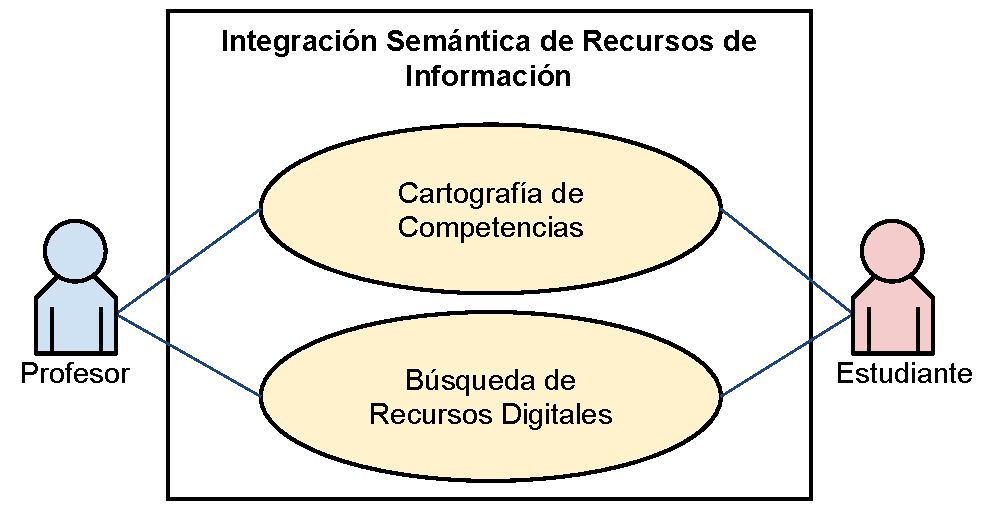
\includegraphics[width=0.6\textwidth]{CasosUso}
\caption{Diagrama de casos de uso para la integraci�n de los recursos de una memoria corporativa.}
\label{fig:cdu}
\end{figure}

La descripci�n de estos casos de uso se expresan a continuaci�n.

\subsection{Cartograf�a de Competencias}
El elemento din�mico en el �rea de RyT es el conjunto de personas que se clasifican en: \textit{profesores, investigadores, estudiantes y empleados}. Estas personas tienen actitudes, valores, conocimientos t�cnicos, habilidades individuales y colectivas. Las caracterizadoras profesionales son importantes para la organizaci�n. Porque con base en �stas se pueden identificar las personas para: \textit{realizar determinadas tareas, solucionar problemas espec�ficos, hacer colaboraciones o tener un determinado cargo}.

La \textbf{\textit{cartograf�a de competencias}} es la b�squeda y recuperaci�n de las personas a partir de las caracter�sticas profesionales. Los principales par�metros en la b�squeda de estas personas son: las competencias profesionales (\textit{trabajo en equipo, liderazgo, organizar, planificar}), conocimientos en temas de Redes y Telecomunicaciones (\textit{sistemas operativos, capa enlace, filtros, ontolog�as, radios cognitivos}), capacidades ling��sticas  (\textit{lee en ingl�s, escribe en espa�ol, habla en franc�s}), relaciones profesionales (\textit{colega, asesor o conocido}) y finalmente por la ocupaci�n (\textit{estudiante, empleado o profesor}).

Para cada \textit{persona} identificada en la memoria corporativa, debe ser recuperada \textit{informaci�n significativa} de �sta. La finalidad esto, es proporcionar al usuario mayor informaci�n, para que pueda localizar y contactar a la persona o filtrar los resultados de acuerdo a otros criterios (\textit{sexo, edad, habilidades}).

\subsection{B�squeda de Recursos Digitales}
En la memoria corporativa de RyT, los recursos digitales representan \textit{ideas, objetos, teor�as, procesos, flujos de trabajo y conocimiento est�tico de la organizaci�n} en un formato digital. Estos recursos se clasifican en: \textit{art�culos cient�ficos, libros, reportes t�cnicos, p�ginas web, tesis, otros documentos, audios, v�deos, presentaciones, im�genes y otros archivos multimedia}. Las personas emplean a estos recursos como \textit{objetos de aprendizaje}. Por esta raz�n, deben identificarse los recursos que solucionen las \textit{necesidades informativas} de los usuarios.

La \textbf{\textit{b�squeda de recursos digitales}} es la b�squeda y recuperaci�n de los documentos y archivos multimedia a partir del contenido de �stos. Los principales par�metros de b�squeda de los recursos digitales son: el autor, la extensi�n (\textit{ppt, wav, mp3, mpg, jpg}), relaciones con los temas de Redes y Telecomunicaciones (\textit{sistemas operativos, capa enlace, filtros, ontolog�as, radios cognitivos}), el idioma fuente (\textit{ingl�s, espa�ol, franc�s. ruso, chino}), tipo de recurso digital (\textit{art�culos, reportes t�cnicos, p�ginas web, tesis, libros, audios, v�deos, im�genes y presentaciones}) y la organizaci�n a la que pertenece (\textit{uam, unam, ipn, iee, acm, oracle}).

Para cada \textit{recurso digital} identificado en la memoria corporativa, debe recuperarse informaci�n significativa de �ste, con la finalidad de proporcionar al usuario mayor informaci�n. De esta manera, el usuario verifica la importancia del recursos filtrar los resultados de acuerdo a otros criterios (\textit{n�mero de p�ginas, extensi�n, lenguaje fuente}).

\section{Hip�tesis}
\label{sec:hip} 
En este cap�tulo, se ha descrito de manera expl�cita el alcance, los principales elementos y caracter�sticas para la integraci�n de los recursos en una Memoria Corporativa. Esta integraci�n se ha planteado de manera gen�rica con respecto al uso de una determinada tecnolog�a, con la finalidad de poder desarrollar la integraci�n con alg�n enfoque, herramienta, metodolog�a o aplicaci�n de las Tecnolog�as de la Informaci�n.

Nosotros no elegimos alguna de los dos herramientas que ocupan las personas del �rea (MBSK y GBDR). En cambio, seleccionamos a las Tecnolog�as Sem�nticas como enfoque para solucionar esta integraci�n. De esta manera, \textbf{\textit{nuestra hip�tesis de investigaci�n}} para esta tesis es: \textbf{\textit{�Acaso es posible usar a las Tecnolog�as Sem�nticas para solucionar la integraci�n de los recursos en una memoria corporativa?}}

%En la descripci�n de cada caso se identifican los par�metros de b�squeda de las personas y los recursos digitales. Estos par�metros son las caracter�sticas significativas y las relaciones de �stos. Para visualizar estas caracter�sticas y relaciones, se emplean los \textbf{\textit{diagramas de clase}}.

%El primer diagrama de clase se asocia al caso de uso Cartograf�a de Competencias. En este diagrama el principal elemento es la persona. Con base a la descripci�n de este caso, se identifican las principales caracter�sticas de las personas. 

%El documento auxiliar es: C:\Users\Gatito\Dropbox\Gesti�n Sem�ntica\Actividades 12P\Semana 8 y 9\Anotaciones Sem�nticas.docx
\chapter{Tecnolog�as Sem�nticas}
\label{cap:ets}

Definici�n de tecnolog�as sem�nticas

Sem�ntica

Problemas comunes en no utiliza sem�ntica

La integraci�n tiene varios requisitos indispensables que se enuncian a continuaci�n: 1) Debe permitir consultas espec�ficas de los recursos a partir de sus metadatos. 2) Acceso a todos los recursos. 3) Capacidad de hacer b�squedas complejas. 4) Adaptarse al conocimiento cambiante. 5) Debe ser f�cil de extender. 6) Ser accesible a trav�s de la red. 7) Facilidad de mantener. 8) Emplear tecnolog�as, mecanismos y lenguajes  est�ndar. 

Muchas tecnolog�as de Recuperaci�n de Informaci�n (RI) son adecuadas para construir nuestro sistema. Sin embargo, no todas estas tecnolog�as satisfacen los requisitos que se establecieron al sistema. Un mecanismo para construir bases de conocimiento, son las tecnolog�as sem�nticas.  Las tecnolog�as sem�nticas son una combinaci�n de aplicaciones y especificaciones formales/est�ndares \footnote{M. Bergman, ``Glossary of Semantic Technology Terms,'' Available:  \url{http://www.mkbergman.com/1017/glossary-of-semantic-technology-terms/}}. En donde, estas tecnolog�as se basan en la siguiente idea.  ``El significado de datos y contenidos se almacenan por separado, con la finalidad de tener fluidez en b�squedas y operaciones de los sistemas'' . Estas tecnolog�as sem�nticas permiten agregar una \textit{capa de abstracci�n} sobre las distintas fuentes de informaci�n. Esta capa tiene la finalidad de que tanto personas como aplicaciones entiendan, compartan y procesen eficientemente datos y especificaciones [2]. Nosotros para desarrollar nuestro sistema, optamos por las tecnolog�as sem�nticas, porque estas tecnolog�as proporcionan varios beneficios en la Representaci�n del Conocimiento (KM). A grandes rasgos, estos beneficios son: captar la visi�n de contextos particulares, adaptarse a la naturaleza cambiante del conocimiento,  integraci�n de distintas fuentes de informaci�n, implementaci�n a menor costo, etc. [2][3]A continuaci�n, se discuten detalladamente los beneficios de las tecnolog�as sem�nticas.

La primera tecnolog�a es el Motor de B�squeda. Esta tecnolog�a es com�n para los usuarios que navegan en Internet. Porque los usuarios obtienen varios resultados que pueden responder r�pidamente su consulta. Un Motor de B�squeda es un sistema de recuperaci�n de la informaci�n que a partir de las palabras clave, realiza una b�squeda documental en la Web. Aquellos documentos que contengan las palabras clave, el Motor los regresar� en un listado como respuestas al usuario. La importancia de un Motor es realizar una b�squeda distribuida. Esto quiere decir, los documentos tienen que ser accesibles v�a Web, mediante enlaces URL (Localizador �nico de Recurso).
Nosotros desechamos la tecnolog�a de un motor de b�squeda por varias razones. La principal raz�n son los resultados inesperados. Generalmente, un usuario al hacer una consulta obtiene muchos resultados que no son los esperados. En el peor caso, ning�n resultado responde la pregunta del usuario. Este problema sucede por el funcionamiento basado en las palabras clave y los algoritmos de ranking [5]. Si un motor encuentra documentos con al menos una palabra clave o con las palabras clave muy separadas, entonces estos documentos figurar�n en los resultados. Al someter estos documentos a un algoritmo de ranking que no utiliza criterios objetivos, �stos pueden quedar mal clasificados. En consecuencia, el usuario revisara muchos documentos web hasta que encuentre uno que responda su pregunta. 
Otras razones de no emplear esta tecnolog�a, son los problemas contextuales de las palabras (polisemia y sinonimia). La polisemia se da cuando dos o m�s palabras que se escriben y suenan igual, tienen distinto significado. Por ejemplo, si se hace una pregunta con la palabra ?radio? los resultados de la b�squeda ser�n sobre distintos contextos (geometr�a, anatom�a, qu�mica y telecomunicaciones). Por otro lado, la sinonimia sucede cuando palabras que se escriben de distinta manera, tienen el mismo significado. Por ejemplo, si en una consulta se emplea la palabra ?computadora?, se espera que entre los resultados puedan aparecer documentos con las palabras computador, pc, ordenador o host. Finalmente, podemos decir que empleando este enfoque, los Motores de B�squeda no hacen uso de lenguajes de consulta expresivos y precisos.


2	B�squeda basada en la sem�ntica
El enfoque tradicional tiene una limitante en la recuperaci�n de resultados relevantes para los usuarios, es por esta raz�n que es necesario emplear m�todos o herramientas provenientes de la Web Sem�ntica (extensi�n de la web tradicional). Donde ?la informaci�n escrita en lenguaje natural  cuenta con un significado bien definido, permitiendo que las  computadoras y las personas trabajen en colaboraci�n facilitando la interacci�n entre ambos elementos (computadora y usuario)? \cite{OntoTecRrpKnw}.

Los motores de b�squeda rastrean autom�ticamente gran parte del contenido de la web copiando p�ginas web e indexando su contenido completo, por lo que normalmente encuentran un n�mero inabarcable de resultados para cualquier b�squeda que no sea demasiado rebuscada, e incorporan distintos y cada vez m�s sofisticados procedimientos para decidir en qu� orden sirven esta informaci�n. Los motores de b�squeda est�n concebidos para dedicarse a eso, no a buscar en informaci�n estructurada. Por otra parte, y esto tiene a�n m�s importancia, sus procedimientos no encuentran las p�ginas din�micas generadas a partir de la consulta de informaci�n, as� que no permiten penetrar en la web oculta que tales p�ginas configuran.

Las b�squedas en la Web, en definitiva, dan habitualmente como resultado un enorme n�mero de ocurrencias en muchos casos irrelevantes, que requieren un costoso filtrado manual por parte del usuario. Los motores de b�squeda pueden tener problemas, pero la mayor parte de la frustraci�n que provoca la b�squeda de informaci�n en la red viene de los propios datos. Las razones son tres: los datos no est�n bien catalogados (no tienen metadatos o �stos son sospechosos), no contienen informaci�n sem�ntica legible por la m�quina, o bien su calidad (su pertinencia desde el punto de vista del usuario) es �nfima.

En primera instancia, se debe consultar el t�rmino ?sem�ntica?, definido por el diccionario de la Real Academia Espa�ola como ``El estudio del significado de los signos ling��sticos y de sus combinaciones, desde un punto de vista sincr�nico o diacr�nico''.

La Web sem�ntica es un �rea prolifera, situada en la confluencia de la inteligencia artificial y las tecnolog�as Web, que propone nuevas t�cnicas y paradigmas para representaci�n de la informaci�n y el conocimiento, facilitar tanto el localizar como el compartir, integrar y recuperar recursos [2].

La Web Sem�ntica, basada en conjunto datos procesables por las m�quinas, integrar� un conjunto tecnolog�as dise�adas para posibilitar una nueva visi�n la web, permitir� el razonamiento autom�tico, la gesti�n conocimiento, la mejora del comercio electr�nico y la b�squeda de informaci�n de manera eficaz y precisa.

Web sem�ntica aboga por clasificar, dotar de estructura y anotar los recursos con sem�ntica expl�cita procesable  por m�quinas. Actualmente la Web se asemeja a un grafo formado por nodos del mismo tipo, y arcos (hiperenlaces) igualmente indiferenciados [4]. La Web sem�ntica ha sido estructurada por niveles, estableciendo una jerarqu�a de abstracci�n y dependencias entre los distintos niveles.

�Para que tener un integrador sem�ntico de los recursos? Si existen buscadores como Google, Bing o Yahoo. Para responder est� pregunta se emplea el siguiente ejemplo al buscar ?Profesores con conocimientos en radios cognitivos?, los resultados que arrojan cualquiera de los motores de b�squeda antes citados; no hay alg�n recurso del tipo persona (profesor) con conocimientos en radios cognitivos. Por el contrario se tienen distintos resultados asociados a distintos contextos (Qu�mica, Comunicaciones, Medio de comunicaci�n, Anatom�a, o Geometr�a), porque la palabra radio tiene m�ltiples significados (homonimia). De est� manera al emplear un sistema de interacci�n sem�ntica de los recursos de una memoria corporativa, los resultados ser�n los adecuados como los esbozado en la siguiente figura.

1.2	Web Sem�ntica
?Es una Web dotada de mayor significado (sem�ntica) en la que cualquier usuario en Internet podr� encontrar respuestas a sus preguntas de forma m�s r�pida y sencilla gracias a una informaci�n mejor definida? [2].
?La Web Sem�ntica ayuda a resolver problemas importantes, de esta manera las personas delegan tareas a los procesos autom�ticos y estos son capaces de procesar el contenido de los recursos, razonar sobre �ste, combinarlo y realizar deducciones l�gicas para resolver problemas autom�ticamente, como la integraci�n los recursos? [2].
Existen tres elementos de la web sem�ntica que permiten tener bien definido el significado de los datos. Estos elementos son ontolog�a, descripci�n sem�ntica y lenguaje de consulta.


\section{Ontolog�a}
\label{sec:onto} 
Qu� es una ontolog�a

Describir por qu� es importante

Cuales son sus caracter�sticas
1) Describir conocimiento y 2) Explotar el conocimiento con fines de b�squeda de informaci�n.

Las ontolog�as representan el conocimiento contenido en los sitios de internet, definiendo formalmente los diferentes dominios mediante clasificaciones de conceptos y sus relaciones asociadas, a la vez que proporcionan mecanismos l�gicos para poder realizar deducciones sobre este conocimiento.

En la web sem�ntica, se necesita que el conocimiento est� representado de forma que sea legible por los computadores, est� consensuado, y sea reutilizable, las ontolog�as proporcionan la v�a para representar este conocimiento. El �xito de la Web sem�ntica, seg�n sus impulsores, se materializar� en parte por la disposici�n a compartir ontolog�as que muestren comunidades y grupos en la web.

La palabra Ontolog�a ha sido tomada de la filosof�a, y se define como una explicaci�n sistem�tica de la existencia. En el campo de la Inteligencia Artificial, (para Neches y colegas) una Ontolog�a define los t�rminos b�sicos y las relaciones comprendidas en el vocabulario de un �rea tem�tica as� como las reglas para combinar t�rminos y relaciones que permita definir extensiones del vocabulario. De acuerdo con esta definici�n, una ontolog�a no s�lo incluye los t�rminos definidos expl�citamente en ella, sino tambi�n aquellos t�rminos que pueden ser deducidos a trav�s de reglas. La definici�n de Gruber \cite{Gruber} es ``una Ontolog�a es una especificaci�n explicita de una conceptualizaci�n'' se convierte en la definici�n m�s referenciada en la literatura. Borst modifica sutilmente la definici�n de Gruber diciendo que: ``Las Ontolog�as son  definidas como una especificaci�n formal de una conceptualizaci�n compartida''.

Estas dos definiciones han sido explicadas por Studer y colegas: ``Conceptualizaci�n se refiere a un modelo abstracto de alg�n fen�meno en el mundo identificando los conceptos relevantes de dicho fen�meno. Explicita significa que los tipos de conceptos usados y las restricciones que sobre ellos se dan est�n definidos expl�citamente. Formal se refiere al hecho que una ontolog�a deber�a ser comprensible por la maquina. Compartida se refiere a la idea de que una ontolog�a captura un conocimiento consensuado, esto es, la ontolog�a no es privada para alg�n individuo, debe ser aceptada por un grupo''.

Es un conjunto de conceptos, propiedades, relaciones y restricciones entre los conceptos para un �rea de conocimiento (vocabulario conceptual); una ontolog�a de dominio sirve para que las personas y procesos autom�ticos entiendan los conceptos y relaciones, adem�s estos procesos a partir de la ontolog�a hacen inferencias para generar nuevo conocimiento. Con base en los conceptos se pueden definir las caracter�sticas de los recursos, en donde est�s caracter�sticas se denominan metadatos; estos pueden hacer referencia al entorno de un recurso (autores, nombre y apellidos, t�tulo, publicaci�n, tipos de recurso, fecha de creaci�n, fecha de nacimiento, URI  etc.) � al contenido del mismo (keywords, fecha de nacimiento, tel�fono, abstract, direcci�n, referencias, etc.). La siguiente figura muestra algunos de los metadatos que podemos asociar a una persona (concepto).

Una ontolog�a se define como ?un conjunto de conceptos pertenecientes a un dominio particular?. En donde estos conceptos est�n bien definidos, est�n jerarquizados, tienen relaciones y restricciones con otros conceptos. Para describir las ontolog�as, los lenguajes est�ndar son el OWL (Lenguaje de Ontolog�as Web) y el RDF(S) (Esquema del Marco de Descripci�n de Recursos). Donde el lenguaje m�s expresivo y que a�ade m�s vocabulario es OWL.

Es un conjunto de conceptos, propiedades, relaciones y restricciones entre los conceptos para un �rea de conocimiento (Vocabulario conceptual). Otra definici�n m�s formal de ontolog�a es ?una red conceptual que incluye un conjunto completo de conceptos y nociones para describir un dominio espec�fico, en donde los conceptos est�n vinculados entre s� por relaciones taxon�micas y por la sem�ntica? [A survey of semantic web standards to representing knowledge in problem solving situations].

El concepto de ontolog�a naci� en la filosof�a, pero su definici�n fue adaptada para las tecnolog�as de la informaci�n y con el paso de los a�os �sta ha ido evolucionando. Una ontolog�a es modelo de datos y l�gico que representa un conjunto de conceptos y relaciones de los mismos para un determinado dominio [2]. Las ontolog�as son formales, explicitas, expresivas y compartidas [6], con la finalidad de explotar el conocimiento impl�cito y expl�cito.

\section{Marco de Descripci�n de Recursos (RDF)}
Qu� es RDF
RDF es un modelo est�ndar para el intercambio de datos en la Web. RDF tiene caracter�sticas que facilitan la combinaci�n de datos incluso si los esquemas subyacentes son diferentes, y espec�ficamente apoya la evoluci�n de esquemas en el tiempo sin necesidad de que todos los consumidores de datos a ser cambiados.

Todo recurso tiene un URI

Que es triple
RDF extiende a la estructura de enlace de la Web para utilizar a URIs para nombrar la relaci�n entre las cosas, as� como los dos extremos de la conexi�n (lo que se conoce normalmente como "triple"). El uso de este modelo simple, que permite que los datos estructurados y semiestructurados ser mezclado, expuestos y compartidos a trav�s de diferentes aplicaciones.

Esta estructura de vinculaci�n forma un un grafo dirigido y etiquetado, donde los bordes representan el llamado enlace entre dos recursos. Este punto de vista gr�fico es el modelo mental m�s f�cil posible para RDF y se utiliza a menudo en las explicaciones f�ciles de entender.

Algo m�s factible ser�a tratar de catalogar la informaci�n de forma descentralizada, a�adiendo cada vez que se incorpora un documento a la red, datos sobre los datos: Metadatos.

Estos tres tipos conceptos forman parte de una sentencia (tripleta) en el modelo RDF y a continuaci�n se describen estos [11] [12].
o	Sujeto: Son aquellos recursos que puede ser descritos (documentos, personas, objetos, lugares, etc.)
o	Predicado: Es una caracter�stica, atributo o relaci�n que se describe de un sujeto (tiene el nombre, naci� en, pertenece a, etc.)
o	Objeto: Es un valor (cadena, entero, fecha) u otro recurso que describe el predicado.

La finalidad de las descripciones sem�nticas es que tanto personas como procesos autom�ticos entiendan el significado de los recursos y de esta manera los usuarios o procesos autom�ticos mejoren su referencia y su recuperaci�n.

una descripci�n sem�ntica representa las caracter�sticas significativas de un recurso. Estas caracter�sticas pueden hacer referencia al entorno de un recurso (autores, nombre y apellidos, t�tulo, publicaci�n, tipos de recurso, fecha de creaci�n, fecha de nacimiento, URL  etc.) o al contenido de los mismos (keywords, fecha de nacimiento, tel�fono, abstract, direcci�n, referencias, etc.).

El Marco de Descripci�n de Recursos (RDF). Este modelo de datos RDF permite transformar literalmente cualquier cosa a una forma can�nica RDF (est�ndar). La unidad b�sica de RDF son las aserciones. La estructura b�sica de una aserci�n es como la de una oraci�n sencilla, es decir, un sujeto, predicado y un objeto. De esta manera, opciones sencillas como ?Juan come pizza? permiten la construcci�n de vocabularios complejos [4]. RDF es el modelo de datos que permite representar el conocimiento de un dominio particular. Los dominios son grandes y poseen una gran cantidad de cosas.

Estas cosas se interconectan con otras, bajo determinada caracter�stica. Entonces para visualizar el conocimiento, es necesario emplear una estructura gr�fica. Esta estructura grafica permite una mejor comprensi�n del conocimiento y brinda est� serie de ventajas [4]: 1) coherencia al navegar sobre el modelo, 2) Inferir sobre el conocimiento, 3) conexi�n con informaci�n relacionada, 4) Mapeo conceptual, 5) marco de trabajo para eliminar ambig�edad en el contexto y 6) vocabulario conceptual y 7) capacidad de representar/conectar cualquier tipo de informaci�n, gracias a los URI.

Estas descripciones sem�nticas tienen un identificador �nico de recurso (URI).

La sintaxis de RDF se compone de una de una sentencia � tripleta (sujeto, predicado y objeto) [5] que expresa el significado de las cosas. Los elementos de la tripleta son los siguientes:
o	Sujeto: Son aquellos recursos que puede ser descritos (documentos, personas, objetos, lugares, etc.)
o	Predicado: Es una caracter�stica, atributo � relaci�n que se describe de un sujeto (tiene el nombre, naci� en, pertenece a, etc.)
o	Objeto: Es un valor (cadena, entero, fecha) u otro recurso que describe el predicado.
La estructura general de RDF es un grafo dirigido, estructurado con nodos y aristas que representan la tripleta. El sujeto es el nodo de origen, el objeto es el nodo de destino y el predicado es la etiqueta de la arista.

Este ABox tambi�n se denomina informaci�n extensional o explicita de la base de conocimiento. 

?	Clase: es una colecci�n de objetos que comparten caracter�sticas comunes. Las clases en una otolog�a tambi�n se conocen como conceptos, colecciones o tipos de cosas.
Persona a Class
Hombre a Class
Mujer a Class
?	Individuo: es un objeto concreto de una clase, como personas, animales, y otros objetos abstractos. Los individuos tambi�n se conocen como instancias o miembros.
Erik a Hombre
Scarlett a Mujer
Juan a Persona
?	Propiedad Objeto: es una relaci�n entre instancias. 
Erik tienePadre Juan
Erik tieneHerman Scarlett
Scarlett tiene.pariente Juan
?	Propiedad Dato: es la relaci�n entre un individuo y un valor  de dato.
Juan tieneEmail ?juan@example.com?^^string
Erik nombreCompleto ?Erik Alarc�n?^^string
Scarlett tieneEdad ?18?^^integer

El modelo de datos RDF permite representar a los recursos en una ontolog�a, con la finalidad de que los procesos autom�ticos interpreten adecuadamente el significado de cada recurso. Esta representaci�n se hace a partir de los metadatos de los recursos. En donde, un metadatos proporciona informaci�n sobre alg�n aspecto o caracter�stica de un recurso. Por ejemplo, nombre del recurso, extensi�n, autor, temas clave, fecha de creaci�n, idioma, etc.  
El modelo RDF establece que cada metadato sea representado en forma de una aserci�n (triple) [4]. El triple es una afirmaci�n de la forma: sujeto, predicado y objeto. El sujeto es el nombre del recurso (individuo), el predicado es el nombre de una relaci�n y el objeto es el nombre de un individuo o valor. Por ejemplo, Pablo vive-en ?Antonio Caso No. 34 cp 12323?, Pablo conoce-a Pedro, Pablo tiene-g�nero masculino, Pedro habla espa�ol, etc. 
El conjunto de aserciones de un individuo, se conoce como descripci�n sem�ntica. Las descripciones sem�nticas poseen tres tipos de aserciones. Estos tres tipos son los siguientes: 1) asignaci�n del nombre del recurso a una determinada clase, 2) relaci�n del nombre del recurso con otro individuo, mediante una Propiedad Objeto y 3) una relaci�n que vincula al nombre del recurso con un valor, mediante una Propiedad Dato. Un ejemplo de una descripci�n sem�ntica, en donde aparecen los tres tipos de aserciones, es el siguiente:
Erik rdf:type Hombre
Erik nombreCompleto ?Erik Alarc�n?^^string
Erik tieneEdad ?18?^^integer
Erik tienePadre Juan
Erik estudiaEn UAM
Erik tieneHabilidadEn WebSem�ntica
Erik tieneEmail ?cbi2@xanum.uam?^^string
Existen muchas sintaxis para representar los triples o aserciones. El W3C establece como est�ndar el RDF/XML1 y obviamente al modelo de datos RDF [10] para representar a los recursos. Finalmente, un dato interesante es el siguiente. El conjunto de descripciones sem�nticas de los recursos es un subconjunto del ABox. 


\section{Lenguaje de consulta sobre grafos RDF (SPARQL)}
Muchos motores de b�squeda, por ejemplo, ahora examinar las p�ginas Web para tipos particulares de metadatos, un tipo de informaci�n que describe otra informaci�n. Un tipo de metadatos se puede especificar a un motor de b�squeda que una serie de n�meros es un n�mero de tel�fono o direcci�n f�sica, mientras que otro tipo puede marcar un bloque de texto como una opini�n de usuario de una empresa o producto.

Son ?un conjunto de �rdenes, operadores y estructuras que, organizadas seg�n unas normas l�gicas, permiten la consulta de fuentes y recursos de informaci�n electr�nica? [6]. Pero no cualquier lenguaje se puede emplear, es necesario uno que permita interrogar las descripciones sem�nticas y encontrar aquellos recursos que satisfagan la consulta del usuario. El lenguaje de consulta basado en la sintaxis RDF y propuesto por la W3C y la WS es SPARQL. 
Las consultas SPARQL se basan en patrones ?triple? en un grafo RDF, estos ?triple? son parecidos a las tripletas RDF, con la diferencia que alguno de los elementos sujeto u objeto son variables. De est� manera al emplear un motor SPAQRL, este debe regresar los recursos que correspondan a ese patr�n. Pero no solamente SPARQL regresa un recurso, tambi�n permite:
o	Recuperar los recursos empleando las URI.
o	Recupera conjunciones y disyunciones de un grafo RDF.
o	Capacidad de conjuntar partes de grafos.

Una ontolog�a es una fuente valiosa de informaci�n de los recursos y del conocimiento impl�cito de estos. Entonces para recuperar la informaci�n de una ontolog�a, se emplean lenguajes de consulta especializados. El lenguaje SPARQL5 es el est�ndar propuesto por el W3C para consultar triples. SPARQL funciona a partir de patrones. Estos patrones son similares a los triples, pero a diferencia de estos �ltimos, en un patr�n el sujeto, predicado y objeto puede ser una variable. De esta manera, SPARQL empareja el patr�n con todas las triples de la ontolog�a. Aquellas triples concordantes, SPARQL recuperar� el valor o valores asociados con la variable o variables.
Un ejemplo b�sico de consulta es  ?busca a qui�nes tengan habilidad en Web Sem�ntica?. La expresi�n asociada a esta consulta en lenguaje SPARQL es: 
	SELECT ?x 						WHERE {?x tieneHabilidadEn WebSem�ntica.}
Analizando esta consulta,  la cl�usula SELECT identifica las variables que deben aparecer en los resultados de la consulta. Mientras la cl�usula WHERE proporciona el patr�n que debe concordar con las triples del ABox. Espec�ficamente, la variable ?x contendr� los individuos que tienen como Predicado (tieneHabilidadEn) y como Objeto (WebSem�ntica).  Una soluci�n de esta consulta es el individuo ?Erik?.
SPARQL tambi�n permite ampliar y restringir las consultas sobre las afirmaciones, as� como tambi�n emplear elementos del componente terminol�gico (TBox). Los siguientes ejemplos muestran las restricciones que se pueden hacer en una consulta:
?	?Encontrar el correo de todas las mujeres?.
SELECT ?mail					WHERE{							?y rdf:type Mujer.						?y tieneEmail ?mail.				}
?	?Encontrar las personas que estudian en la UAM y son mayores de 18 a�os?.
SELECT ?x						WHERE {							?x tieneEdad ?age.						FILTER (?age > 18)					?x estudiaEn UAM.				}
?	?Encontrar las personas que son casadas?.
SELECT ?name					WHERE{							{?name tieneEsposa ?x.}					UNION							{?name esEsposaDe ?x.}			}
M�s detalles de consultas complejas en SPARQL, revisar el documento SPARQL5 Lenguaje de consulta para RDF.

Todas las aserciones del Abox deben ser almacenadas de forma permanente, con la finalidad de hacer futuras consultas sobre estos triples. El triplestore es el mecanismo que nos permite gestionar (almacenamiento y b�squeda) los triples. Un triplestore robusto de permitir el almacenamiento nativo de triples, carga y procesamiento del grafo RDF en memoria, consultar los valores de los triples y hacer inferencias a partir de los axiomas. 


\section{Reglas de inferencia (RDF(S)/OWL) y razonadores}
Las interpretaciones de las frases que no tienen sentido pueden ser filtrados mediante inferencia, que a veces se utiliza para clasificar las posibilidades de diferentes interpretaciones tambi�n. F�rmulas para la comprensi�n del lenguaje pueden ser creados usando modelos, en los que las variables matem�ticas son asignados a diferentes elementos ling��sticos. Las letras P y Q se utilizan a menudo con la teor�a de la prueba, en el que las f�rmulas se pueden derivar de otros con la ayuda de reglas de inferencia. Inform�tica palabras en una oraci�n a veces ayuda a obtener significados o encontrar otras alternativas.

El prop�sito de la sem�ntica computacional es representar las ambig�edades o frases que pueden tener diferentes significados, de manera superficial. Tambi�n implica palabras de procesamiento que dependen de contexto debe entenderse. El objetivo es por lo general para interpretar un significado autom�ticamente, as� como para relacionar el m�todo de hacerlo, para otros procesos computacionales para llevarse a cabo de manera m�s eficiente.

Si bien una ontolog�a permite definir un vocabulario com�n entre personas y procesos, tambi�n se puede explotar est� para generar nuevo conocimiento mediante el uso de procesos que hacen inferencia. En donde la tarea de inferir nuevo conocimiento a partir de sentencias � reglas se le denomina razonamiento, entonces un programa razonador es aquel que permite hacer inferencias y generar conocimiento, mediante el uso de un motor de inferencia (IE) y un conjunto de reglas (axiomas). El motor de inferencia  puede ser descrito como una forma de m�quina de estados finitos con un ciclo que consta de tres estados: coinciden las reglas, selecci�n de reglas y ejecutar reglas. En el primer estado el motor encuentra todas las reglas que satisfacen con el contenido actual de datos almacenados. El segundo estado aplica alguna estrategia para determinar que reglas realmente va ejecutar y el tercer estado ejecuta estas reglas

La tarea de inferir nuevo conocimiento a partir de sentencias � reglas se le denomina razonamiento, entonces un programa razonador es aquel que permite hacer inferencias y generar conocimiento, mediante el uso de un motor de inferencia (IE) y un conjunto de reglas (axiomas).

En donde inferir en la Web Sem�ntica significa que los procesos autom�ticos generen nuevas relaciones basadas en los datos y la informaci�n adicional en forma de un vocabulario, por ejemplo, un conjunto de reglas. Donde las Reglas definen un mecanismo general para el descubrimiento y generaci�n de nuevas relaciones basadas en las existentes.

El TBox proporciona reglas o axiomas para proporcionar el conocimiento implico. A continuaci�n se listan varios de estos axiomas.
?	Jerarqu�a de clases y propiedades, cosiste en agrupar jer�rquicamente y sistem�ticamente las diferentes clases y propiedades en grupos estables. La operaci�n b�sica es ?subclase? y consiste en ligar un concepto/relaci�n particular con un concepto/relaci�n general.
Persona rdfs:subClassOf Thing
Mujer rdfs:subClassOf Persona 
tienePadre rdfs:subProprertyOf tieneParinete
?	Dominio y Rango de una Propiedad Objeto, son las clases que intervienen en una relaci�n. En donde el primer componente de una Propiedad es el Dominio y el segundo el Rango.
tieneEsposa rdfs:Domain Hombre
tieneEsposa rdfs:Range Mujer
?	Dominio y Rango de una Propiedad Dato, son las clases y tipos de valores que intervienen en una relaci�n. Para m�s detalles de estos tipos de valores consultar el RDF Primer 2.
nombreCompleto rdfs:Domain Persona
nombreCompleto rdfs:Range xsd:string
?	Caracter�sticas de las Propiedades Objeto, existen muchas relaciones en el mundo real, como transitividad, funcionalidad, simetr�a, inversa, y otras. Entonces, aquellas propiedades que tengan el comportamiento de las relaciones antes descritas, se debe especificar que son de este tipo.  Afortunadamente, existen axiomas que permiten hacer esto. Para m�s detalles de estas caracter�sticas consultar el tutorial ?Una Gu�a para construir Ontolog�as OWL? [9].
nombreCompleto rdf:type owl:FunctionalProperty
tienehijo rdf:type owl:AsymmetricProperty
tienePariente rdf:type owl:TransitiveProperty
?	Restricci�n existencial, se emplea para asegurar que al menos un individuo que se obtiene por una propiedad, pertenece a la clase especificada. Por ejemplo, el axioma para decir que ?todos tienen una madre que es mujer? es:
tieneMadre some Mujer
?	Restricci�n universal, se emplea para asegurar que todos los individuos que se obtienen por una propiedad, pertenecen a la clase especificada. Por ejemplo, el axioma para decir que ?todos tienen solo parientes humanos? es:
tienePariente only Humano
?	Restricci�n cardinal, se emplea para asegurar que como m�ximo, m�nimo o exactamente ?n? individuos que se obtienen por una propiedad, pertenezcan a la clase especificada. Por ejemplo, el axioma para decir ?todos tienen m�nimo dos parientes mujeres? es:
tienePariente min 2 Mujer 
?	Operadores l�gicos, se emplean para construir axiomas m�s complejos. Los operadores b�sicos son And, Or, Not. En este ejemplo, el axioma  para decir que ?Todas las personas son hombres o mujeres?, es.
Persona rdfs:subClassOf (Hombre or Mujer)
2RDF Primer, disponible en: http://www.w3.org/TR/rdf-primer/, 2004
3OWL 2 Web Ontology Language Primer, disponible en: http://www.w3.org/TR/owl2-primer/, 2012.
4RDF Vocabulary Description Language, disponible en: http://www.w3.org/TR/rdf-schema/, 2004
5SPARQL Query Language for RDF, disponible en: http://www.w3.org/TR/rdf-sparql-query/, 2008
Existen muchos lenguajes para construir una ontolog�a. Sin embarg� no todos estos lenguajes son est�ndares o soportan algunos de los axiomas antes descritos. El World Wide Consortium propone como est�ndares al Lenguaje Web Ontol�gico (OWL3) y al Marco de Descripci�n de Recursos (RDF4). Ambos lenguajes permiten definir clases y varios axiomas, pero el m�s limitado en expresividad es RDF. Aunque el lenguaje OWL se basa en el RDF. Por tal motivo, si se quiere una ontolog�a apegada a lenguajes est�ndares y actualizados, la opci�n a elegir es OWL.


El otro componente denominado componente terminol�gico (TBox), sirve para ?describir los conceptos en t�rminos de otros y las relaciones que hay entre los mismos?

Como bien se ha dicho, una ontolog�a proporciona un formalismo y expresividad para representar el conocimiento. El TBox proporciona los axiomas para representar el conocimiento impl�cito de un dominio. Pero, para aprovechar este conocimiento impl�cito se requiere una aplicaci�n. Este programa se denomina razonador. Un razonador es una pieza de software que permite deducir datos y asociaciones a partir de los axiomas6. Estos razonadores infieren sobre la jerarqu�a de las clases, las relaciones entre clases y las instancias. Los razonadores tambi�n son conocidos como razonadores sem�nticos, motor de inferencias o motor de reglas. 
Los beneficios de emplear los razonadores se describen a continuaci�n.
?	En la fase de construcci�n de un modelo de ontolog�a. El razonador verifica la consistencia del modelo. El objetivo de verificar la consistencia es identificar contradicciones o detalles en el modelo.
?	Un razonador en combinaci�n con SPARQL permite mejorar la calidad de los resultados de las c�nsulas, ya que se aprovecha el conocimiento impl�cito del TBox.
Para hacer claro este �ltimo punto, se emplea el siguiente ejemplo. El ABox tiene estos triples {Elena rdf:type Mujer, Erik rdf:type Hombre y Jorge rdf:type Hombre}y el TBox tiene estos axiomas {Hombre rdfs:subClassOf Persona y Mujer rdfs:subClassOf Persona}. Si se quieren todos los individuos qu� son persona. El patr�n asociado a esta consulta es: ?name rdf:type Persona. Al hacer la consulta SPARQL sin un razonador, la respuesta de SPARQL no arrojar�a ning�n valor. Porque expl�citamente no hay una aserci�n o triple que establezca a un individuo con la clase Persona. Sin embargo, esta misma consulta con un razonador, arrojara los tres individuos  como respuesta. Por los dos axiomas de jerarqu�a. 
Muchos razonadores existentes est�n disponibles en la Web. Pero, varios de �stos ya est�n integrados o son f�ciles de integrar con los entornos de desarrollo integrado (IDE). Los razonadores m�s comunes son Pellet7 y FACT++8, que poseen una licencia open source AGPL version 3 license y LGPL respectivamente.

\section{Ventajas de las tecnolog�as Sem�nticas}
Interoperabilidad y adaptaci�n al conocimiento
El enfoque relacional de las Bases de Datos tiene un esquema relacional e instancias, �stos se pueden traducir a elementos de una Ontolog�a; las tablas ser�an clases, las relaciones entre tablas son propiedades de los objetos, una tupla ser�a un individuo, y los atributos ser�an propiedades de los datos. Con base en estas correspondencias se puede modelar una sencilla Ontolog�a. Sin embargo, para enriquecer una Ontolog�a es necesario considerar la utilidad de la misma (casos de uso) de tal forma que se requiere: introducir relaciones (pertinentes), proponer restricciones (l�gica de primer orden) a los conceptos, definir los conceptos, e inclusive interrogar al propio esquema conceptual. Algo que por el momento el enfoque relacional no tiene. Otra diferencia es que el enfoque relacional tiene el esquema conceptual y los datos juntos (monolito), mientras que en la Web Sem�ntica, los datos y el esquema pueden estar separados. Lo anterior resulta importante porque al tener separados a �stos, se pueden construir esquema e instancias de forma colaborativa; una actividad de la misi�n de la WS. (Hay que cambiar esta idea por: al tener separados el TBox y ABox, porque si evoluciona el conocimiento, podr�amos cambiar algunos axiomas del TBox y as� obtener los resultados deseados o una mejor adaptaci�n al conocimiento).

Colaboraci�n entre usuarios, de tal manera que el conocimiento de distintos miembros o trabajadores contribuya a la reutilizaci�n de los documentos y a la mejora en las anotaciones. De esta manera los usuarios pueden contribuir al aumento de las anotaciones sobre sus documentos, as� como auxiliar a los dem�s miembros para generar o modificar las anotaciones relacionadas a sus recursos, para tener una amplia y mejor memoria de anotaciones. En este ambiente colaborativo los miembros deben ser capaces de ver que anotaci�n se est� empleando para que en ese momento no se trabaje sobre esa, ya que si llega a suceder las anotaciones pueden ser inconsistentes.

4.       Ortiz, M., Institute of Information Systems, V.U. of T.: Introducci�n a las L�gicas Descriptivas. (2009).
9.   	Studer, R. et al.: Knowledge engineering: Principles and methods. Data & Knowledge ngineering. 25, 1-2, 161?197 (1998).
10.   	Kr�tzsch, M. et al.: A Description Logic Primer. CoRR. abs/1201.4, 1?16 (2012).
11.   	M. Horridge et al.: A Practical Guide To Building OWL Ontologies Using The Prot�g�-OWL Plugin and COODE Tools Edition 1.3. The University Of Manchester Stanford University. (2011).

Los objetos, ideas, conceptos est�n en constante cambio. Estos cambios modifican sutilmente la estructura del conocimiento. Algo que en el pasado es verdadero, se vuelve falso en el presente. Esto significa que el conocimiento se adapta y evoluciona [4]. Por tanto, herramientas para la gesti�n del conocimiento, deben adaptar su l�gica a esta naturaleza cambiante [4]. Herramientas como Gestores de Bases de Datos (GBD) no son adaptativas al conocimiento cambiante (sistemas cerrados). Porque los GBD son mecanismos apegados a un esquema est�tico que es r�gido. Por lo tanto, cuando existen cambios en el conocimiento, este esquema debe ser modificado, as� como tambi�n algunas relaciones en la BD. Esta operaci�n es costosa (tiempo, dinero y recursos humanos) y cada vez que evolucione el conocimiento se debe efectuar nuevamente. Las aplicaciones y sistemas adaptables a la ?naturaleza cambiante del conocimiento? deben emplear el paradigma de suposici�n de un mundo abierto (OWA). Este paradigma establece las siguientes premisas [4]: 1) la falta de una aserci�n no implica que sea falso o verdadero, 2) la falta de conocimiento no significa falsedad, 3) todo est� permitido, hasta que se establece que est� prohibido, 4) Esquema es extensible y 5) la informaci�n imperfecta se puede combinar.

El conocimiento es amplio y no est� en centralizado. Tambi�n los usuarios no est�n en una misma ubicaci�n, estos siempre est�n en constante movimiento. Por tal motivo, se necesita una arquitectura que considere esta naturaleza distribuida del conocimiento y de los usuarios. Esta arquitectura debe permitir el acceso uniforme a los recursos [4]. La Web es una arquitectura que proporciona el acceso e intercambio de informaci�n. Espec�ficamente, la Web ofrece los siguientes beneficios [4]: 1) toda la informaci�n es accesible a trav�s de Identificador �nico de Recursos (URI), 2) toda la informaci�n de la Web puede ser integrada, 3) muchas tecnolog�as Web est�n disponibles para su uso y son de c�digo abierto y 4) la Web es escalable, robusta y sustentable. En la Web, hay una amplia variedad de datos. Los datos pueden ser de diferentes formas, como estructurados, semi-estructurados, y no estructurados. En donde, datos estructurados son informaci�n que se apega a un modelo de datos, datos semi-estructurados son informaci�n contenida entre etiquetas u otros lenguajes de marcado, y datos no estructurados es informaci�n orientada al texto [4]. A su vez estos datos se guardan en distintos tipos de archivos, como texto plano, HTML, XML, formas codificadas, o binarios. Por tal raz�n, es necesario modelar la informaci�n (sin importar la forma y formato) en un formato est�ndar.

Las tecnolog�as sem�nticas son flexibles y permiten la interoperabilidad con otros sistemas [3][4]. Un ejemplo de esta interoperabilidad es el siguiente. Los Gestores de Bases de Datos son sistemas cerrados, pero una organizaci�n puede depender exclusivamente de estos. Si se remplaza de  golpe este sistema, entonces se puede desencadenar varios riesgos a la organizaci�n. Una estrategia importante e interesante es aprovechar a estos gestores. Un gestor debe verse como una fuente de datos estructurados. Si se introduce una capa de interoperabilidad sobre estos datos, entonces esta capa transforma los datos a la forma can�nica RDF. Una gran ventaja de tener un modelo de datos flexible y est�ndar, es el desarrollo de aplicaciones gen�ricas. Estas aplicaciones gen�ricas tendr�n como objetivos: una facilidad de uso y una mejor integraci�n de los usuarios. Por lo tanto, personas expertas en el dominio ser�n los principales constructores del grafo de conocimiento [4]. Esta actividad, reducir� costos monetarios, personales y temporales, adem�s la informaci�n del grafo ser� m�s confiable.
\chapter{Estado del arte}
\label{cap:soa}
La \textbf{\textit{integraci�n de los recursos de informaci�n en una memoria corporativa}} ha sido poco explotada por las organizaciones o �reas de investigaci�n. Existen algunos trabajos sobre la \textit{integraci�n de informaci�n} que incorporan a las tecnolog�as sem�nticas para representar y enriquecer el conocimiento de un dominio dado, as� como, la b�squeda de informaci�n a partir de este conocimiento. Los trabajos para este \textit{estado del arte}, son aquellos que cumplen con alguno de estos criterios:

\begin{itemize}
\item Integraci�n de los recursos: es el proceso de b�squeda y recuperaci�n de la informaci�n sobre los recursos de informaci�n. En la secci�n \ref{sec:intdk} se define formalmente este concepto.
\item Memoria corporativa: es la representaci�n del conocimiento en una organizaci�n. En la secci�n \ref{sec:mecor} se define formalmente este concepto.
\item Modelo sem�ntico: es la representaci�n del conocimiento a partir de las tecnolog�as sem�nticas. En la secci�n \ref{sec:rdf} y \ref{sec:reginf} se describe este concepto.
\item Inferencia en el modelo: es el proceso de deducir informaci�n a partir del modelo sem�ntico. En la secci�n \ref{sec:reginf} se define formalmente este concepto.
\item Interfaz de usuario: es la construcci�n de un aplicaci�n visual para que los usuarios pregunten o naveguen a partir  del modelo sem�ntico. En la secci�n \ref{cap:piu} se describen las funciones que debe tener un prototipo para la integraci�n de los recursos.
\end{itemize}

La secci�n \label{sec:eoaisr} describe los trabajos que se estudiaron para la integraci�n de los recursos. Al final de esta secci�n, se presenta una tabla comparativa de estos trabajos y los criterios que �stos cumplen.

En este \textit{estado del arte} se contempla un estudio de las aplicaciones para realizar la \textit{integraci�n sem�ntica de los recursos en una memoria corporativa}. Las aplicaciones estudiadas, se agrupan de acuerdo a las siguientes funcionalidades.

\begin{enumerate}
\item Escribir los declaraciones en forma de triple y guardarlos en alguna sintaxis est�ndar.
\item Escribir los axiomas mediante los vocabularios est�ndar (OWL y RDF(S)).
\item Gesti�n del grafo RDF, es decir, carga del modelo, consulta de informaci�n e inferencia.
\end{enumerate}

En la secci�n \ref{sec:eoats}, se describen estas aplicaciones con base en su funcionalidad. Al final de cada agrupaci�n, se da a conocer: \textit{cu�l herramienta se eligi� para facilitar y efectuar la funcionalidad dada}.

\section{Integraci�n sem�ntica de recursos de informaci�n}
\label{sec:eoaisr}
El principal objetivo de la integraci�n de los recursos es buscar y recuperar informaci�n significativa que est� en los recursos, para responder las necesidades informativas de las personas. Una integraci�n sem�ntica de recursos emplea las tecnolog�as sem�nticas con la finalidad de recuperar informaci�n m�s significativa en los recursos a partir de las caracter�sticas y relaciones de estos. El uso de una memoria corporativa para la integraci�n sem�ntica, se traduce en informaci�n y conocimiento de los recursos bajo un dominio particular.

Algunos trabajos exploran o emplean el enfoque sem�ntico para fines de integraci�n del conocimiento, representaci�n de una memoria corporativa o b�squeda de informaci�n. A continuaci�n, se describe el estado actual del conocimiento referente a estos trabajos.

La \textbf{\textit{arquitectura del modelo dual}} \cite{Archetype} es una propuesta para la representaci�n consistente y comprensible de la informaci�n cl�nica de cualquier persona. La finalidad de esta arquitectura es facilitar el acceso de historial cl�nico de los pacientes a los profesionales de la salud. La informaci�n de estos historiales esta distribuida en varios sistemas independientes y heterog�neos.

Esta arquitectura se basa en separar la representaci�n de la informaci�n y el conocimiento. En la informaci�n se describen las estructuras de datos comunes. Mientras, el conocimiento se especifica con arquetipos que representan el conocimiento formal de conceptos cl�nicos.

Este trabajo presenta una herramienta para desarrollar los arquetipos de datos cl�nicos. Esta herramienta es llamada LinkEHR-Ed. La finalidad de est� es que los profesionales de la salud y expertos en tecnolog�as de la informaci�n sean los principales constructores del conocimiento.

Nosotros \textbf{\textit{elegimos este trabajo}} por las siguientes razones:
1) \textit{la arquitectura representa el conocimiento de los historiales cl�nicos (dominio de la salud)}, 2) \textit{la arquitectura solventa la informaci�n distribuida y formatos propios de un sistema}, 3) \textit{la arquitectura modela el conocimiento a manera de un componente terminol�gico y un componente asertivo}, 4) \textit{los arquetipos agregan una capa sem�ntica y proporcionar el conocimiento formal para el sector salud} y 5) \textit{una herramienta para construir arquetipos asociados al sector salud}.

El marco de integraci�n sem�ntica es una propuesta para solucionar de manera eficaz y flexible la integraci�n de la informaci�n en el dominio del alojamiento en-l�nea. La finalidad de esta integraci�n es facilitar la reuni�n y compartici�n de informaci�n referente al alojamiento en-l�nea.

Este marco de integraci�n se basa en un enfoque sem�ntico y propone el uso de ontolog�as para: 1) facilitar el acceso a la informaci�n, 2) enfrentar la heterogeneidad en la estructura de la informaci�n, 3) resolver la naturaleza din�mica de las fuentes de informaci�n, 4) permitir a los propietarios de informaci�n una participaci�n en el proceso de integraci�n, y 5) emplear una serie de peque�os esquemas para intercambiar la informaci�n.

%%%[04:14:23 p.m.] Carolina Medina: 1.- LA descripci�n de cada trabajo/enfoque (resumen). Por qu� lo seleccion� o incluye [ref]
%%%[04:14:54 p.m.] Carolina Medina: 2.- culminar la secci�n con una tabla comparativa en la cual se pongan
%%%[04:15:35 p.m.] Carolina Medina: Sistemas comparados/ caracter�sticas que tienen o deben de cumplir

\section{Herramientas para la integraci�n sem�ntica de recursos}
\label{sec:eoats}
Un \textbf{\textit{descriptor sem�ntico de recursos}} \cite{Uren:2006} es una herramienta para crear y almacenar tripletas RDF a partir de la \textit{informaci�n expl�cita en los recursos}. Las tripletas que son generadas por esta herramienta, est�n escritas en una de las siguientes sintaxis: \textit{RDF/XML, Turtle, N-triple y N3}. El principal objetivo de un \textit{descriptor} es construir instancias y relacionar �stas con determinados valores u otras instancias (\textit{concepto de triple}). Estas herramientas necesitan un TBox para saber cu�les clases y propiedades, pueden emplearse en los triples. Un descriptor proporciona una \textit{interfaz gr�fica de usuario} (GUI\label{sym:gui}) para simplificar a los usuarios la creaci�n y modificaci�n de las declaraciones. Algunos descriptores sugieren informaci�n para las declaraciones a partir de un proceso de aprendizaje en un corpus documental o de im�genes.

En la siguiente lista, se presentan los descriptores sem�nticos que nosotros estudiamos.
% Estas interfaces tienen un editor de documentos para que un usuario: \textit{1) visualice el contenido de estos, 2) seleccione los datos (literales: cadenas, enteros, flotantes) y 3) asocie los datos a una propiedad}.

\begin{itemize}
\item \textbf{\textit{OntoMat Annotizer}} \cite{OntoBasDoc} es una herramienta para hacer anotaciones sem�nticas de p�ginas web, documentos basados en texto plano y lenguajes de marcado\footnote{M. Siroker, ``OntoMat Annotizer,''  Disponible en: \url{http://projects.semwebcentral.org/projects/ontomat/}}. El objetivo de esta herramienta es que el usuario cree de manera amigable instancias y declaraciones de �stas, mediante la funcionalidad de arrastrar y soltar (drag-and-drop).
\item \textbf{\textit{MnM}} \cite{Uren:2006} es una herramienta que proporciona apoyo automatizado y semiautomatizado para describir p�ginas Web con contenido sem�ntico\footnote{The Open University, ``MnM,''  Disponible en: \url{http://projects.kmi.open.ac.uk/akt/MnM/}}. MnM tiene GUI que integra un editor de ontolog�a, navegador Web, un editor de instancias y de propiedades. El objetivo de esta herramienta es la descripci�n de documentos a partir de declaraciones derivadas de ontolog�as preexistentes.
\item \textbf{\textit{GATE}} \cite{Cunningham2011a} es un entorno de desarrollo integrado (IDE\label{sym:ide}) para el desarrollo de componentes en el procesamiento del lenguaje humano y el procesamiento de texto\footnote{The University of Sheffield, ``GATE,''  Disponible en: \url{http://gate.ac.uk/}}. Las tareas en el procesamiento de texto son: \textit{miner�a web, extracci�n de informaci�n  y descripciones sem�nticas}.
\item \textbf{\textit{Aktive Media}} \cite{Uren:2006} es una GUI para la descripci�n autom�tica de una colecci�n de im�genes o documentos (batch annotation) para un contexto espec�fico. ``\textit{El objetivo de Aktive es automatizar el proceso de descripci�n, mediante la sugerencia interactiva de la informaci�n al usuario, mientras �ste est� describiendo}\footnote{A. Chakravarthy, V. Lanfranchi , F. Ciravegna, ``AKTive Media,''  Disponible en: \url{http://www.aktors.org/technologies/aktivemedia/index.html}}''. Estas sugerencias se hacen con base en axiomas y descripciones previas.
\end{itemize}

La finalidad de un descriptor es facilitar la generaci�n de descripciones en forma de triple. Sin embargo, hay varias razones, por las cu�les, no se elige una de estas herramientas para alcanzar este fin. Las razones son: 1) \textit{todas estas aplicaciones permiten hacer declaraciones de documentos e im�genes, por tal raz�n, no proporcionan una soluci�n a la heterogeneidad en formato}, 2) \textit{OntoMat Annotizer y MnM no interpretan los axiomas que est�n escritos con los vocabularios OWL y RDF(S)}, 3) \textit{Aktive Media y GATE cambian las URIs en las tripletas por sus propios URIs}, 4) \textit{OntoMat Annotizer y MnM no tienen versi�n estable} y 5) \textit{Aktive Media, GATE y MnM no tienen documentaci�n disponible para solucionar problemas de configuraci�n}.

Un \textbf{\textit{script}} es un c�digo que se escribe en un lenguaje de programaci�n y se utiliza para la escritura y almacenamiento de descripciones en forma de tripletas. El prop�sito es facilitar y agilizar el proceso de generaci�n de tripletas en alguna sintaxis est�ndar. Aunque un script no posee una interfaz gr�fica para seleccionar la informaci�n de los recursos. Esto se puede solucionar mediante el uso de formularios web que capturen la informaci�n sobre los recursos. Posteriormente, la informaci�n es guardada en alg�n documento de texto plano, para que un script transforme esta informaci�n en triples RDF. Por tal raz�n, \textbf{\textit{un script es la opci�n electa}} para representar el conocimiento expl�cito en forma de tripletas.\\

Un \textbf{\textit{editor de ontolog�a}} \cite{Tode} es una herramienta que proporciona una serie de interfaces amigables para la construcci�n y mantenimiento de ontolog�as. Estos editores proporcionan las siguientes funcionalidades b�sicas a los usuarios: 1)\textit{definir las clases, propiedades, instancias y axiomas}, 2) \textit{cargar, almacenar, importar y exportar ontolog�as que son escritas con lenguajes est�ndar (RDF(S)y OWL)} y 3) \textit{visualizar las clases, propiedades e individuos}.

\begin{itemize}
\item \textbf{\textit{Prot�g�}} \cite{protege} es una plataforma con herramientas para la creaci�n, visualizaci�n y manipulaci�n de ontolog�as en diversos formatos de representaci�n\footnote{Stanford Center for Biomedical Informatics Research, ``Prot\'{e}g\'{e},''  Disponible en: \url{http://protege.stanford.edu/}}. Esta plataforma proporciona al usuario una interfaz amigable para la definici�n de clase, propiedades y axiomas, as� como la introducci�n de datos. La arquitectura de esta herramienta se puede extender a trav�s de plug-ins y APIs. Esta herramienta tiene licencia open-source Mozilla Public License\footnote{Mozilla, ``Mozilla Public License,''  Disponible en: \url{http://www.mozilla.org/MPL/}}.
\item \textbf{\textit{pOWL}} \cite{pow} es una herramienta para la visualizaci�n y edici�n de ontolog�as v�a web\footnote{S\"{o}ren Auer, ``pOWL,''  Disponible en: \url{http://aksw.org/Projects/Powl.html}}. Esta herramienta soporta la carga y edici�n de ontolog�as con vocabularios RDF(S) y OWL, generaci�n de consultas y almacenamiento del modelo en una base de datos relacional.
\item \textbf{\textit{TopBraid Composer}} \cite{OntologyManagement} es un IDE para "\textit{desarrollar, gestionar y probar configuraciones de los modelos de conocimiento e instancias de las bases de conocimiento}"\footnote{TopQuadrant, Inc., ``TopBraid Composer,''  Disponible en: \url{http://www.topquadrant.com/products/TB_Composer.html}}. Esta herramienta proporciona un conjunto de editores para visualizar grafos RDF y diagramas de clase. Existen tres versiones de esta herramienta: maestro, est�ndar y gratuita. La versi�n gratuita permite crear y editar archivos OWL/XML, as� como consultar con el lenguaje SPARQL.
\item \textbf{\textit{SWOOP}} \cite{swoop} es un editor para crear y editar ontolog�as, comprobar inconsistencias, navegar por las ontolog�as, compartir y reutilizar los datos existentes\footnote{University of Maryland, ``SWOOP,''  Disponible en: \url{https://code.google.com/p/swoop/downloads/list}}. Este editor ofrece un entorno con aspecto de navegador web para facilitar la navegaci�n y edici�n de ontolog�as OWL. Este editor provee una interfaz amigable y eficaz para los usuarios web promedios.
\end{itemize}

%Prot�g� se puede extender sus funcionalidades a trav�s de plug-ins y APIs. Estas funcionalidades son: 1) visualizar los axiomas, clases y propiedades en forma de grafo, 2) exportar ontolog�as a una variedad de formatos, 3) importar y hacer uso de alg�n motor de inferencia o razonador, 4) cambiar el URI del vocabulario, 5) exportar las ontolog�a a otras sintaxis (RDF/XML, Turtle, Manchester), por mencionar algunas.

\textbf{\textit{Prot�g�}} es el editor electo para representar los axiomas en una ontolog�a. Porque este editor proporciona estos beneficios: 1) \textit{una interfaz amigable e intuitiva para el usuario}, 2) \textit{amplia documentaci�n y tutoriales, as� como una comunidad de desarrolladores}, 3)\textit{facilidad de extender la funcionalidad de esta herramienta, gracias a su arquitectura de plug-ins}, 4) \textit{variedad de sintaxis para las ontolog�as, como: Turtle, Manchester, OWL/XML o XML/RDF}, 5) \textit{visualizaci�n del grafo (axiomas, clases y propiedades)}, 6) \textit{incorporar razonadores, como: Pellet\footnote{Clark \& Parsia, LLC, ``Pellet,''  Disponible en: \url{http://clarkparsia.com/pellet/}}, Fact++\footnote{Clark \& Parsia, LLC, ``Pellet,''  Disponible en: \url{http://clarkparsia.com/pellet/}} y HermiT\footnote{Oxford University, ``HermiT,''  Disponible en: \url{http://hermit-reasoner.com/}}} y 
7) \textit{incorporar un motor de consulta SPARQL}.\\

Un \textbf{\textit{triplestore}} \cite{dbpedia_2012} es un programa para \textit{el almacenamiento e indexaci�n de tripletas RDF}, con el fin de permitir la consulta eficiente de informaci�n sobre estas tripletas. Estos triplestores emplean el est�ndar SPARQL como lenguaje de consulta para consultar el grafo RDF. Algunos triplestores soportan la capacidad de inferir en el grafo RDF a partir de axiomas, mediante la incorporaci�n o importaci�n de un razonador para ello. Los triplestores se idealizan como \textit{sistema gestor de bases de datos para modelos basados en triplestas RDF}.

En el siguiente listado, se presentan y describen los triplestores que estudiamos.

\begin{itemize}
\item \textbf{\textit{Apache Jena}} \cite{McBride} es un \textit{marco de trabajo} que  proporciona un conjunto de interfaces de programaci�n de aplicaciones (API\label{sym:api}) para Java. Estas APIs ofrecen las siguientes funcionalidades: \textit{lectura, procesamiento y escritura de triples RDF, as� como axiomas RDF(S) y OWL, un motor de inferencia y un motor de consulta SPARQL}. La finalidad de Jena es desarrollar aplicaciones que usan las tecnolog�as sem�nticas para la representaci�n del conocimiento\footnote{The Apache Software Foundation, ``Apache Jena,''  Disponible en: \url{http://jena.apache.org/}}.%%%Estas APIs tienen las siguientes funcionalidades: 1) \textit{lectura, procesamiento y escritura de triples RDF en alguna sintaxis est�ndar (RDF/XML, N-triples y turtle)}. 2) soporte de axiomas en los lenguajes OWL y RDF(S), 3) \textit{un motor de inferencia que soporta axiomas en OWL y RDF(S)}, 4) \textit{almacenamiento eficiente de los triples en el disco duro} y 5) \textit{un motor de consultas con soporte para el lenguaje SPARQL}.
\item \textbf{\textit{Stardog}} \cite{stardog} es una base de datos para modelos sem�nticos. El prop�sito de esta herramienta es la ejecuci�n de consultas sobre los datos RDF que est�n bajo su gesti�n directa\footnote{Clark \& Parsia, LLC, ``Stardog,''  Disponible en: \url{http://stardog.com/}}. Esta herramienta emplea los protocolos \textit{HTTP  y SNARL} para \textit{acceder y controlar de manera remota el modelo de datos RDF, inferencia a partir de axiomas en lenguaje OWL} y \textit{consultas SPARQL}. %%%Stardog soporta el lenguaje est�ndar SPARQL y emplea los protocolos \textit{HTTP  y SNARL} para: acceder y controlar de manera remota el modelo de datos RDF, la inferencia y el an�lisis de datos en el lenguaje OWL. Stardog apoyado en el motor de b�squeda de texto Lucene, proporciona la capacidad de b�squedas sem�nticas que consiste en la indexaci�n de literales RDF.
\item \textbf{\textit{4store}} \cite{Fstore} \textit{es un sistema para el almacenamiento RDF que incorpora un motor de consultas SPARQL}\footnote{Garlik, ``4store,''  Disponible en: \url{http://4store.org/}}. Las principales fortalezas de esta herramienta son el rendimiento, seguridad, escalabilidad y estabilidad.
\item \textbf{\textit{Sesame}} \cite{Sesame} \textit{es un \textit{marco de trabajo} est�ndar de facto para el an�lisis, almacenamiento, inferencia y consulta de datos RDF}\footnote{Aduna, ``Sesame,''  Disponible en: \url{http://www.openrdf.org/index.jsp}}. Este marco proporciona una API que puede emplearse sobre los distintos \textit{sistemas de almacenamiento RDF} para consultar y acceder a esta informaci�n de manera remota. %Finalmente, Sesame soporta: los principales sintaxis para los triples RDF y el lenguaje de consulta SPARQL.
\end{itemize}

Cualquiera de estos triplestore es una opci�n viable para efectuar tareas de almacenamiento y b�squeda de informaci�n en grafos RDF. Aunque, el m�s interesante desde nuestra perspectiva es Apache Jena. Las razones del \textit{porqu� emplear esta herramienta}, son: 1) \textit{amplia documentaci�n y tutoriales para el desarrollo de modelos sem�nticos}, 2) \textit{integraci�n de Jena en IDEs para el lenguaje Java, como Eclipse}\footnote{The Eclipse Foundation, ``Eclipse IDE,''  Disponible en: \url{http://www.eclipse.org/}}, 3) \textit{proyecto open-source bajo la licencia Apache\footnote{The Eclipse Foundation, ``Licencia Apache v. 2.0 ,''  Disponible en: \url{http://www.apache.org/licenses/LICENSE-2.0.html}} versi�n 2}, 4) \textit{un conjunto de librer�as para crear, cargar, almacenar y consultar declaraciones, as� como axiomas en OWL y RDF(S)}, 5) \textit{un motor de inferencia para realizar razonamiento en ontolog�as que emplean axiomas OWL y RDF(S)} y 6) \textit{una amplia comunidad de desarrolladores}.

%%%Fuentes: C:\Users\Gatito\Dropbox\Gesti�n Sem�ntica\Actividades 12P\Semana 8 y 9\Anotaciones Sem�nticas.docx

%%%C:\Users\ARTE\Dropbox\Gesti�n Sem�ntica\Actividades 13I\feedback\CMED_8_FEB_Integracion Sem�ntica de los recursos.docx

% TABLA ONTOLOGIAS en: C:\Users\Gatito\Dropbox\Gesti�n Sem�ntica\Actividades 12P\Semana 10\doc auxiliar.docx

\chapter{Integraci�n sem�ntica de recursos de informaci�n en una memoria corporativa}
\label{cap:sir}
%revizar este documento C:\Users\Gatito\Dropbox\Gesti�n Sem�ntica\Tarea12O\Integracion Sem�ntica de los recursos.doc
La \textit{integraci�n de los recursos} es el proceso de b�squeda y recuperaci�n significativa de informaci�n existente en los recursos, para responder una consulta dada por un usuario. Si esta integraci�n se hace mediante el uso de herramientas, est�ndares, metodolog�as y aplicaciones pertenecientes a las \textit{tecnolog�as sem�nticas}, entonces, se dice que �sta es una \textbf{\textit{integraci�n sem�ntica de los recursos (ISR\label{sym:isr})}}.

Esta \textit{integraci�n sem�ntica de recursos} se emplea en una \textit{memoria corporativa (MC)}, porque una memoria tiene un conjunto diverso de recursos de informaci�n que representan el conocimiento de una organizaci�n (dominio particular). Las principales razones para realizar esta \textit{integraci�n en una memoria corporativa}, son las siguientes: 1) \textit{solucionar la heterogeneidad de los recursos y la ambig�edad de la informaci�n en una memoria corporativa}, 2) \textit{adaptar el conocimiento cambiante o explosivo en los recursos}, 3) \textit{extender y mantener un modelo (representaci�n) del conocimiento}, 4) \textit{permitir consultas espec�ficas a partir de las caracter�sticas y relaciones de los recursos}, 5) \textit{recuperar informaci�n significativa de los recursos para que respondan las preguntas de las personas adscritas en la organizaci�n} y 6) \textit{emplear herramientas, aplicaciones, vocabularios y formatos est�ndar}.

El desarrollo de la \textit{integraci�n sem�ntica de recurso} se hace con base en una \textbf{\textit{secuencia ordenada de m�todos (metodolog�a)}}. Esta tesis describe una \textbf{\textit{propuesta de metodolog�a}} para la \textit{integraci�n sem�ntica de recursos en una memoria corporativa}, la cual es guiada por \textit{casos de uso}. La finalidad de esta propuesta es \textit{facilitar y guiar a los desarrolladores en las tareas de construcci�n  de un modelo sem�ntico, as� como en la b�squeda de informaci�n sobre �ste}. Mientras, los principales objetivos de �sta son:

\begin{itemize}
\item realizar la ISR en cualquier memoria corporativa, por ejemplo \textit{Biom�dica, Qu�mica, Biolog�a, Computaci�n, Econom�a, Zoolog�a, por mencionar algunas}
\item emplear distintos \textit{casos de uso} para la ISR y no limitar el n�mero de �stos.
\item representar una MC en un formato est�ndar con un vocabulario consensuado y asociado al contexto de la MC.
\item utilizar vocabularios est�ndares para los axiomas, as� como el uso del lenguaje SPARQL para las consultas.
\end{itemize}

Esta metodolog�a est� organizada en tres etapas principales:

\begin{enumerate}
\item \textbf{\textit{Representaci�n del conocimiento en los recursos}} consiste en identificar los recursos de la memoria corporativa y representar los metadatos (conocimiento expl�cito) de estos recursos mediante el marco RDF.
\item \textbf{\textit{Enriquecimiento del conocimiento en el modelo}} consiste en introducir axiomas en OWL y RDF(S) para extender, completar y adaptar el conocimiento expl�cito de los recursos.
\item \textbf{\textit{B�squeda y recuperaci�n de la informaci�n en el modelo}} consisten en identificar las principales consultas de los usuarios en el dominio y ejecutar �stas mediante el uso de un \textit{motor de b�squeda SPARQL} junto con un \textit{razonador}, para recuperar informaci�n de los recursos.
\end{enumerate}

En esta metodolog�a, uno de los elementos clave es el \textbf{\textit{caso de uso}}. Porque este elemento gu�a el desarrollo de la integraci�n sem�ntica. En concreto, los casos de uso permiten lo siguiente para las tres etapas: 1) \textit{qu� caracter�sticas y relaciones son significativas}, 2) \textit{qu� reglas de inferencia son necesarias} y 3) \textit{cu�les consultas son importantes}.

La Figura \ref{fig:arq} muestra la arquitectura para la \textit{integraci�n sem�ntica de recursos}. Esta arquitectura es gen�rica para ser desarrollada e implementada en cualquier memoria corporativa. Los componentes de esta arquitectura se construyen, utilizan e implementan mediante el uso de nuestra propuesta de metodolog�a.

\begin{figure}[!htb]
\centering
%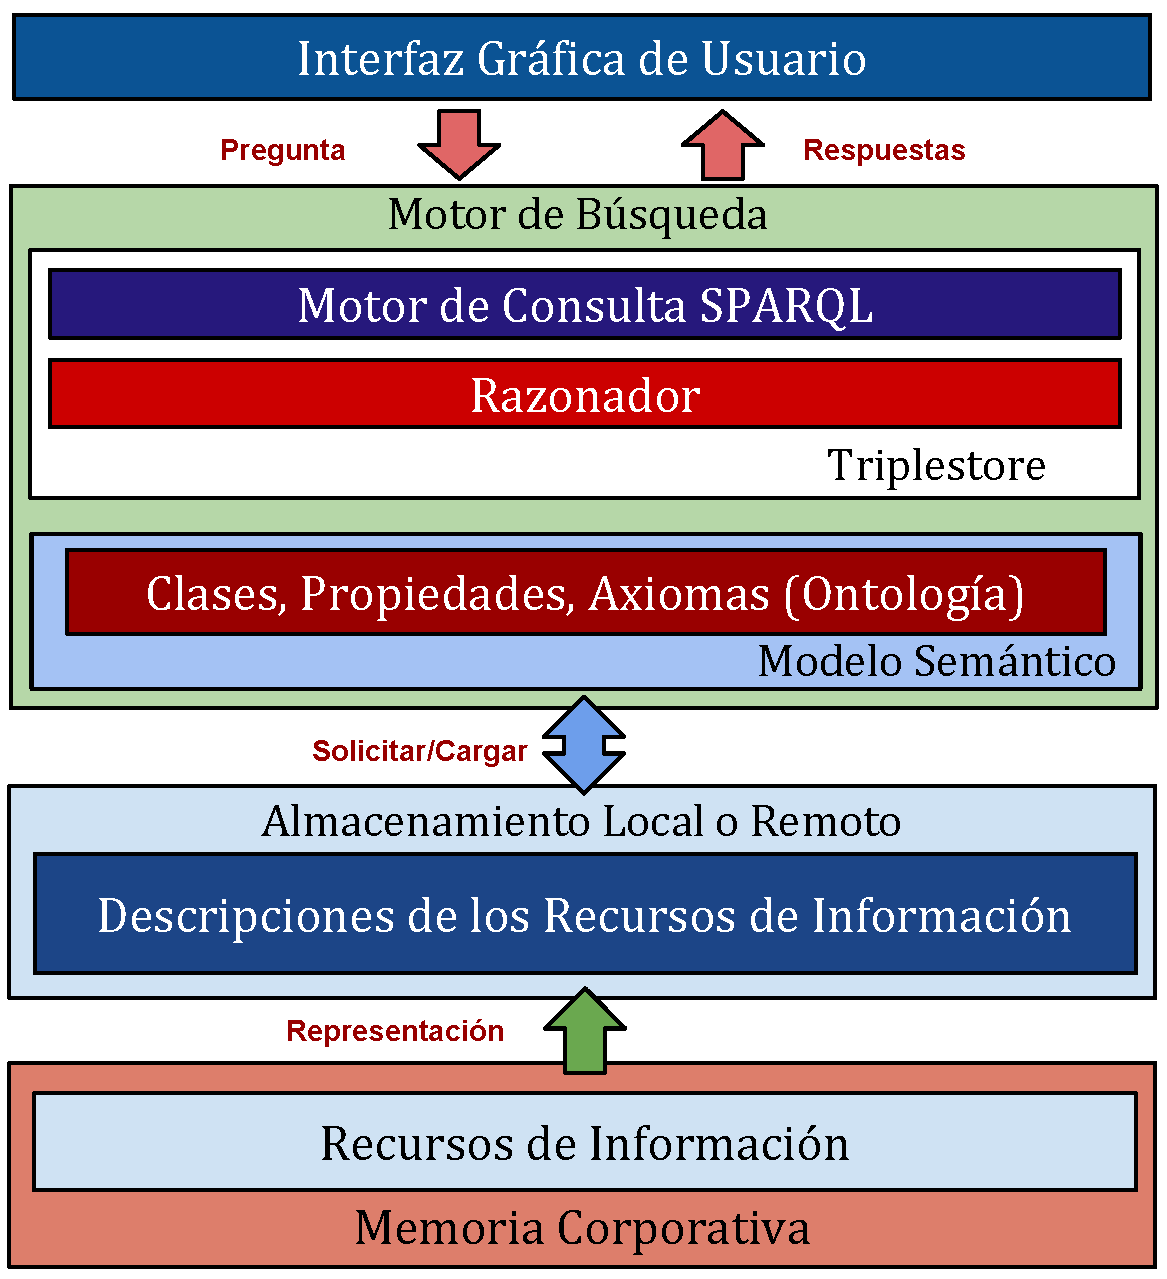
\includegraphics[width=3.2in]{Arquitectura}
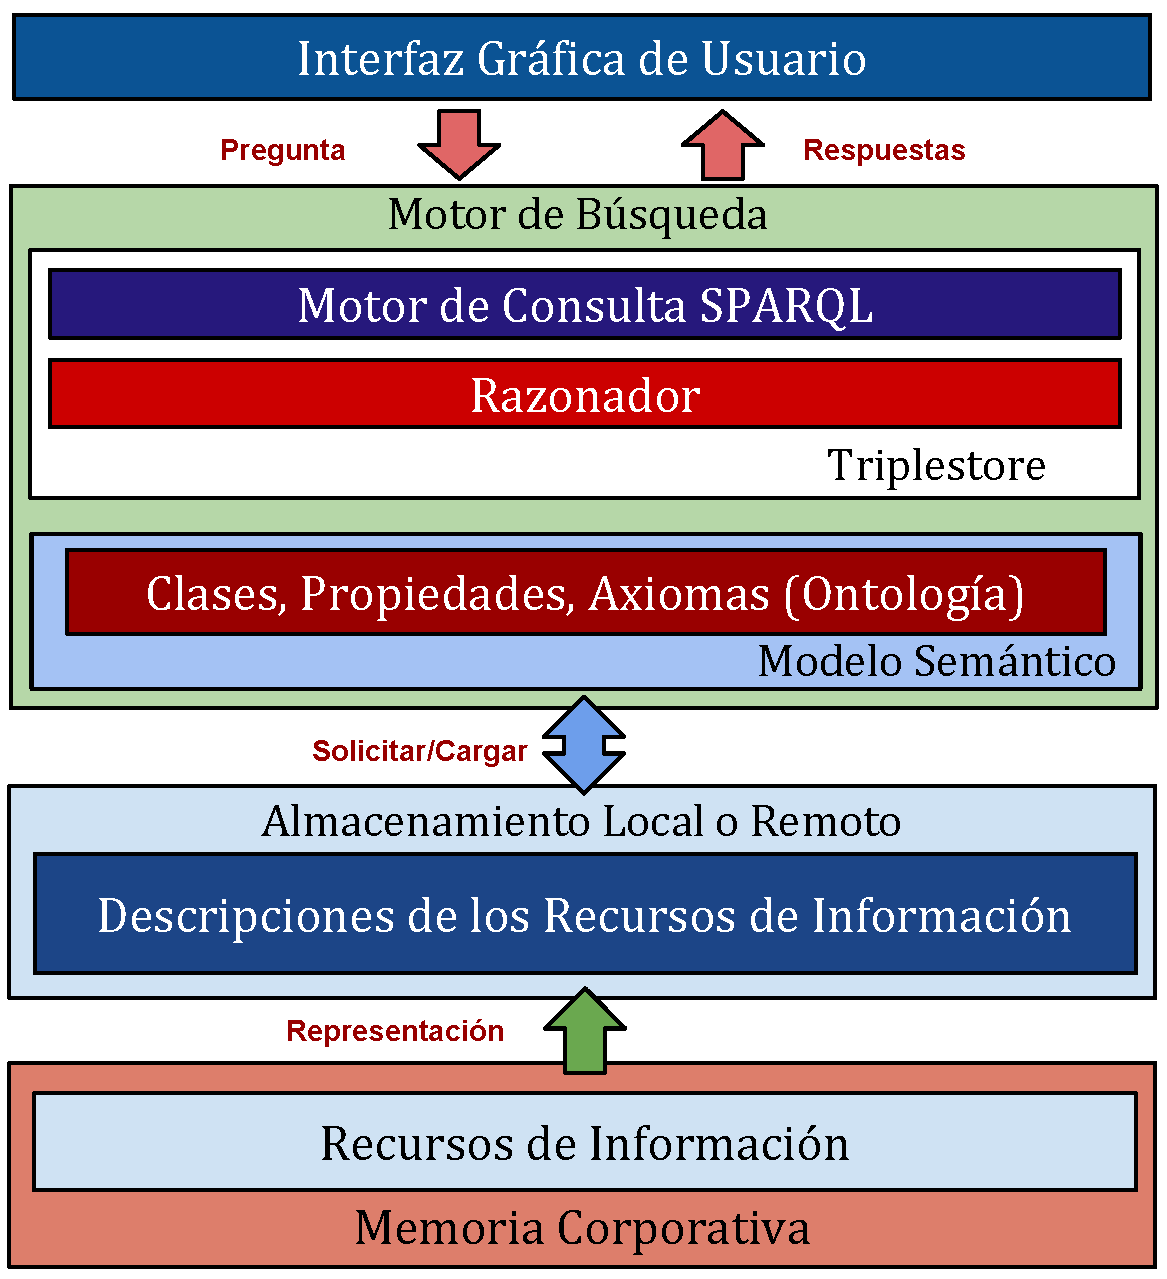
\includegraphics[width=0.6\textwidth]{Arquitectura}
\caption{Arquitectura general para la Integraci�n Sem�ntica de Recurso en una Memoria Corporativa.}
\label{fig:arq}
\end{figure}

Esta arquitectura se dise�o con base en el modelo de tres capas: \textbf{\textit{usuario, negocio}} y \textbf{\textit{datos}}.

\begin{itemize}
\item En la capa de usuario: se tiene un conjunto de p�ginas Web din�micas y est�ticas que proporcionan la interfaz visual. Esta interfaz proporciona una manera f�cil y sencilla de estructurar las preguntas de los usuarios, as� como la visualizaci�n de los resultados vinculados a estas preguntas. Las p�ginas est�ticas proporcionan los formularios para que los usuarios \textit{estructuren las preguntas} y \textit{capturen la informaci�n} a buscar en la MC. Mientras, las p�ginas din�micas proporcionan la informaci�n que responde las preguntas en un formato visual agradable al usuario.
\item En la capa de negocios: una aplicaci�n transforma la informaci�n recopilada de las p�ginas est�ticas en patrones tripletas y construir una consulta SPARQL. Posteriormente, esta aplicaci�n invoca al triplestore para efectuar estas actividades: 1) solicitar y cargar la ontolog�a, 2) hacer inferencia en una ontolog�a mediante el uso de un razonador y 3) buscar y recuperar la informaci�n en el modelo inferido mediante el uso de motor de b�squeda SPARQL y la consulta SPARQL.
\item En la capa de datos (conocimiento): la ontolog�a modela el conocimiento de los recursos de una memoria corporativa en un formato est�ndar y con un vocabulario consensual. El componente asertivo contiene las descripciones de las caracter�sticas y relaciones expl�citas de los recursos. Mientras, el componente terminol�gico contiene los axiomas que definen y restringen la manera en que se relacionan los recursos.
\end{itemize}

Esta propuesta de metodolog�a se pone en pr�ctica para la \textit{memoria corporativa} del grupo de investigaci�n perteneciente al �rea de Redes y Telecomunicaciones del departamento de Ingenier�a El�ctrica de la Universidad Aut�noma Metropolitana Unidad Iztapalapa. Mientras, los \textit{casos de uso} usados en esta propuesta, son \textit{la cartograf�a de competencias} y \textit{la b�squeda de recursos digitales}. Los principales usuarios en la integraci�n son los profesores-investigadores del n�cleo del �rea de Redes y Telecomunicaciones, as� como los estudiantes que realizan alg�n proyecto o servicios social y que son asesorados por un profesor del n�cleo.

%%Mientras la recuperaci�n consiste en consultar el modelo resultante mediante un motor SPARQL y un razonador los triples del grafo RDF.
%%%La integraci�n integraci�n sem�ntica se efect�a en una memoria corporativa (MC), porque esta integraci�n considera algunas caracter�sticas importantes de una memoria corporativa como: 1) el crecimiento explosivo de recursos, 2) heterogeneidad en formato, contenido y estructura de los recursos, 3) ambig�edades en la informaci�n, 4) evoluci�n del conocimiento en los recursos (agregar, eliminar, modificar o renovar), entre otras.
%Pero, para casos pr�cticos, nuestra propuesta se pone en pr�ctica para el grupo de investigaci�n en el �rea de Redes y Telecomunicaciones del depto. de Ingenier�a El�ctrica de la Universidad Aut�noma Metropolitana Unidad Iztapalapa. Mientras, los casos de uso son: la cartograf�a de competencias y la b�squeda de recursos digitales.
\section{Representaci�n del conocimiento en los recursos}
%La etapa de representaci�n consiste en identificar y recopilar los recursos de la memoria corporativa, adquirir el conocimiento de los recursos a partir de las caracter�sticas y relaciones de �stos, representar este conocimiento mediante el uso del marco RDF.
%% El primer paso en la representaci�n es la adquisisci�n, identificaci�n, caracterizaci�n y representaci�n de los recursos
La primera actividad en esta etapa es identificar los requerimientos de la integraci�n de informaci�n para la memoria corporativa, es decir, se deben analizar, encontrar y escribir los casos de uso.

La ``\textit{cartograf�a de competencias} y la \textit{b�squeda de recursos digitales}'' son los dos casos de uso b�sicos para la memoria corporativa del �rea de redes y telecomunicaciones. La descripci�n de la cartograf�a y b�squeda son descritas a continuaci�n.

\begin{enumerate}
\item La \textbf{\textit{cartograf�a de competencias}} es la b�squeda y recuperaci�n de las personas a partir de las caracter�sticas profesionales. Los principales par�metros en la b�squeda de estas personas son: las competencias profesionales (\textit{trabajo en equipo, liderazgo, organizar, planificar}), conocimientos en temas de Redes y Telecomunicaciones (\textit{sistemas operativos, capa enlace, filtros, ontolog�as, radios cognitivos}), capacidades ling��sticas  (\textit{lee en ingl�s, escribe en espa�ol, habla en franc�s}), relaciones profesionales (\textit{colega, asesor o conocido}) y finalmente por la ocupaci�n (\textit{estudiante, empleado, investigador o profesor}).
\item La \textbf{\textit{b�squeda de recursos digitales}} es la b�squeda y recuperaci�n de los documentos y archivos multimedia a partir del contenido de �stos. Los principales par�metros de b�squeda de los recursos digitales son: el autor, la extensi�n (\textit{ppt, wav, mp3, mpg, jpg}), relaciones con los temas de Redes y Telecomunicaciones (\textit{sistemas operativos, capa enlace, filtros, ontolog�as, radios cognitivos}), el idioma fuente (\textit{ingl�s, espa�ol, franc�s. ruso, chino}), tipo de recurso digital (\textit{art�culos, reportes t�cnicos, p�ginas web, tesis, libros, audios, v�deos, im�genes y presentaciones}) y la organizaci�n a la que pertenece (\textit{uam, unam, ipn, iee, acm, oracle}).
\end{enumerate}

La Figura \ref{fig:mccu} muestra los recursos de informaci�n de la memoria corporativa del �rea de Redes y Telecomunicaciones (RyT), los cuales est�n clasificados con base en los dos casos de uso.

\begin{figure}[!htb]
\centering
%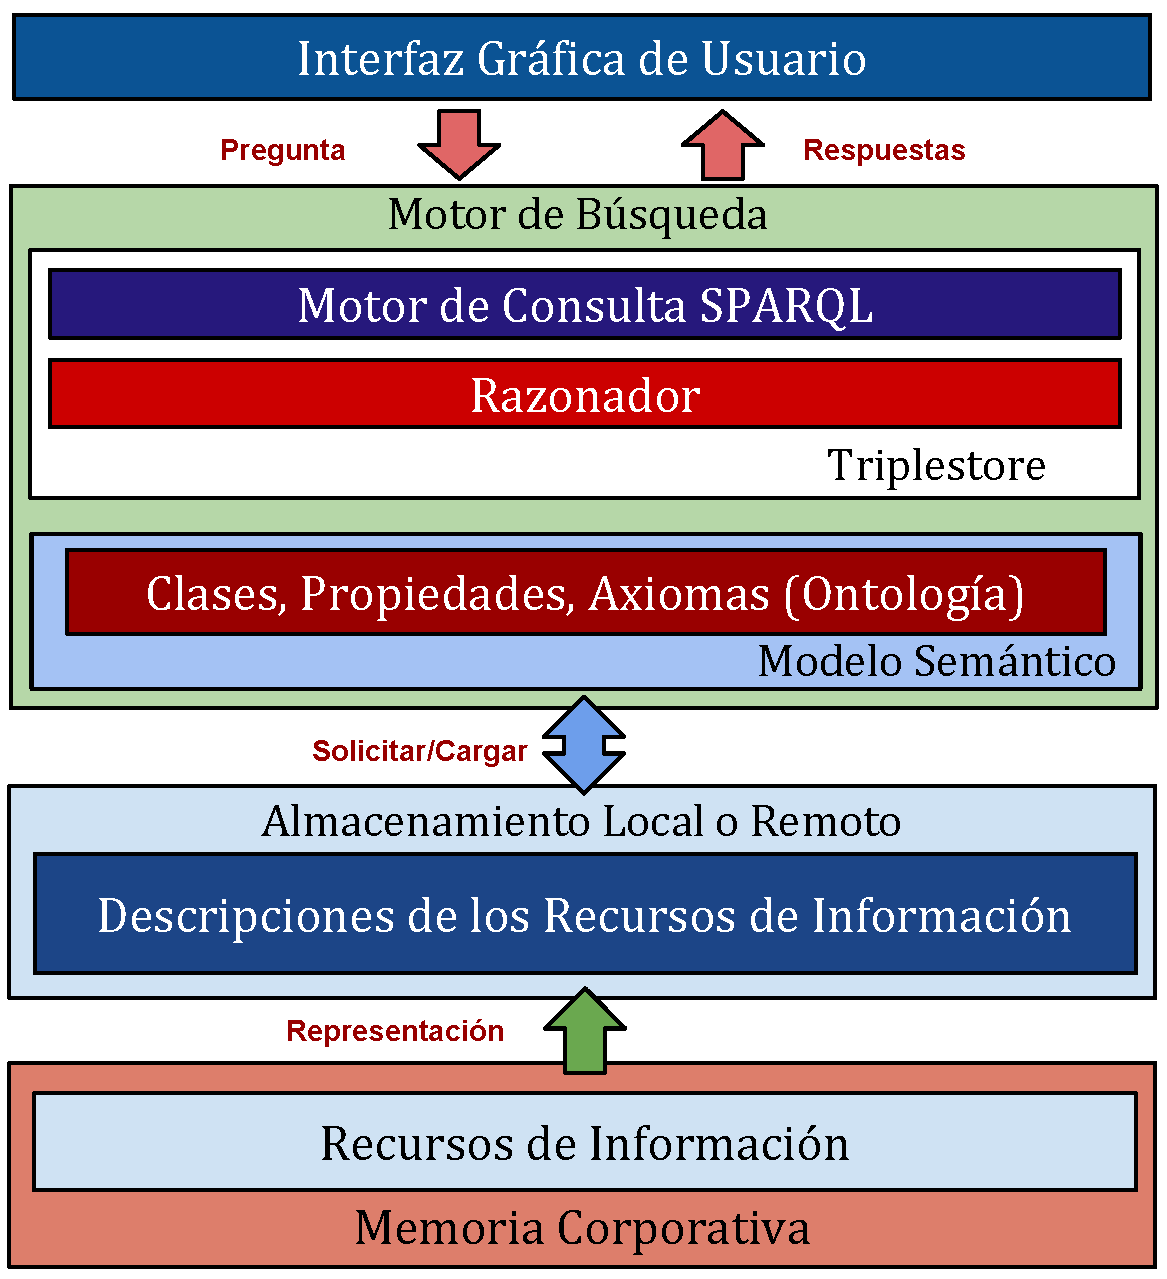
\includegraphics[width=3.2in]{Arquitectura}
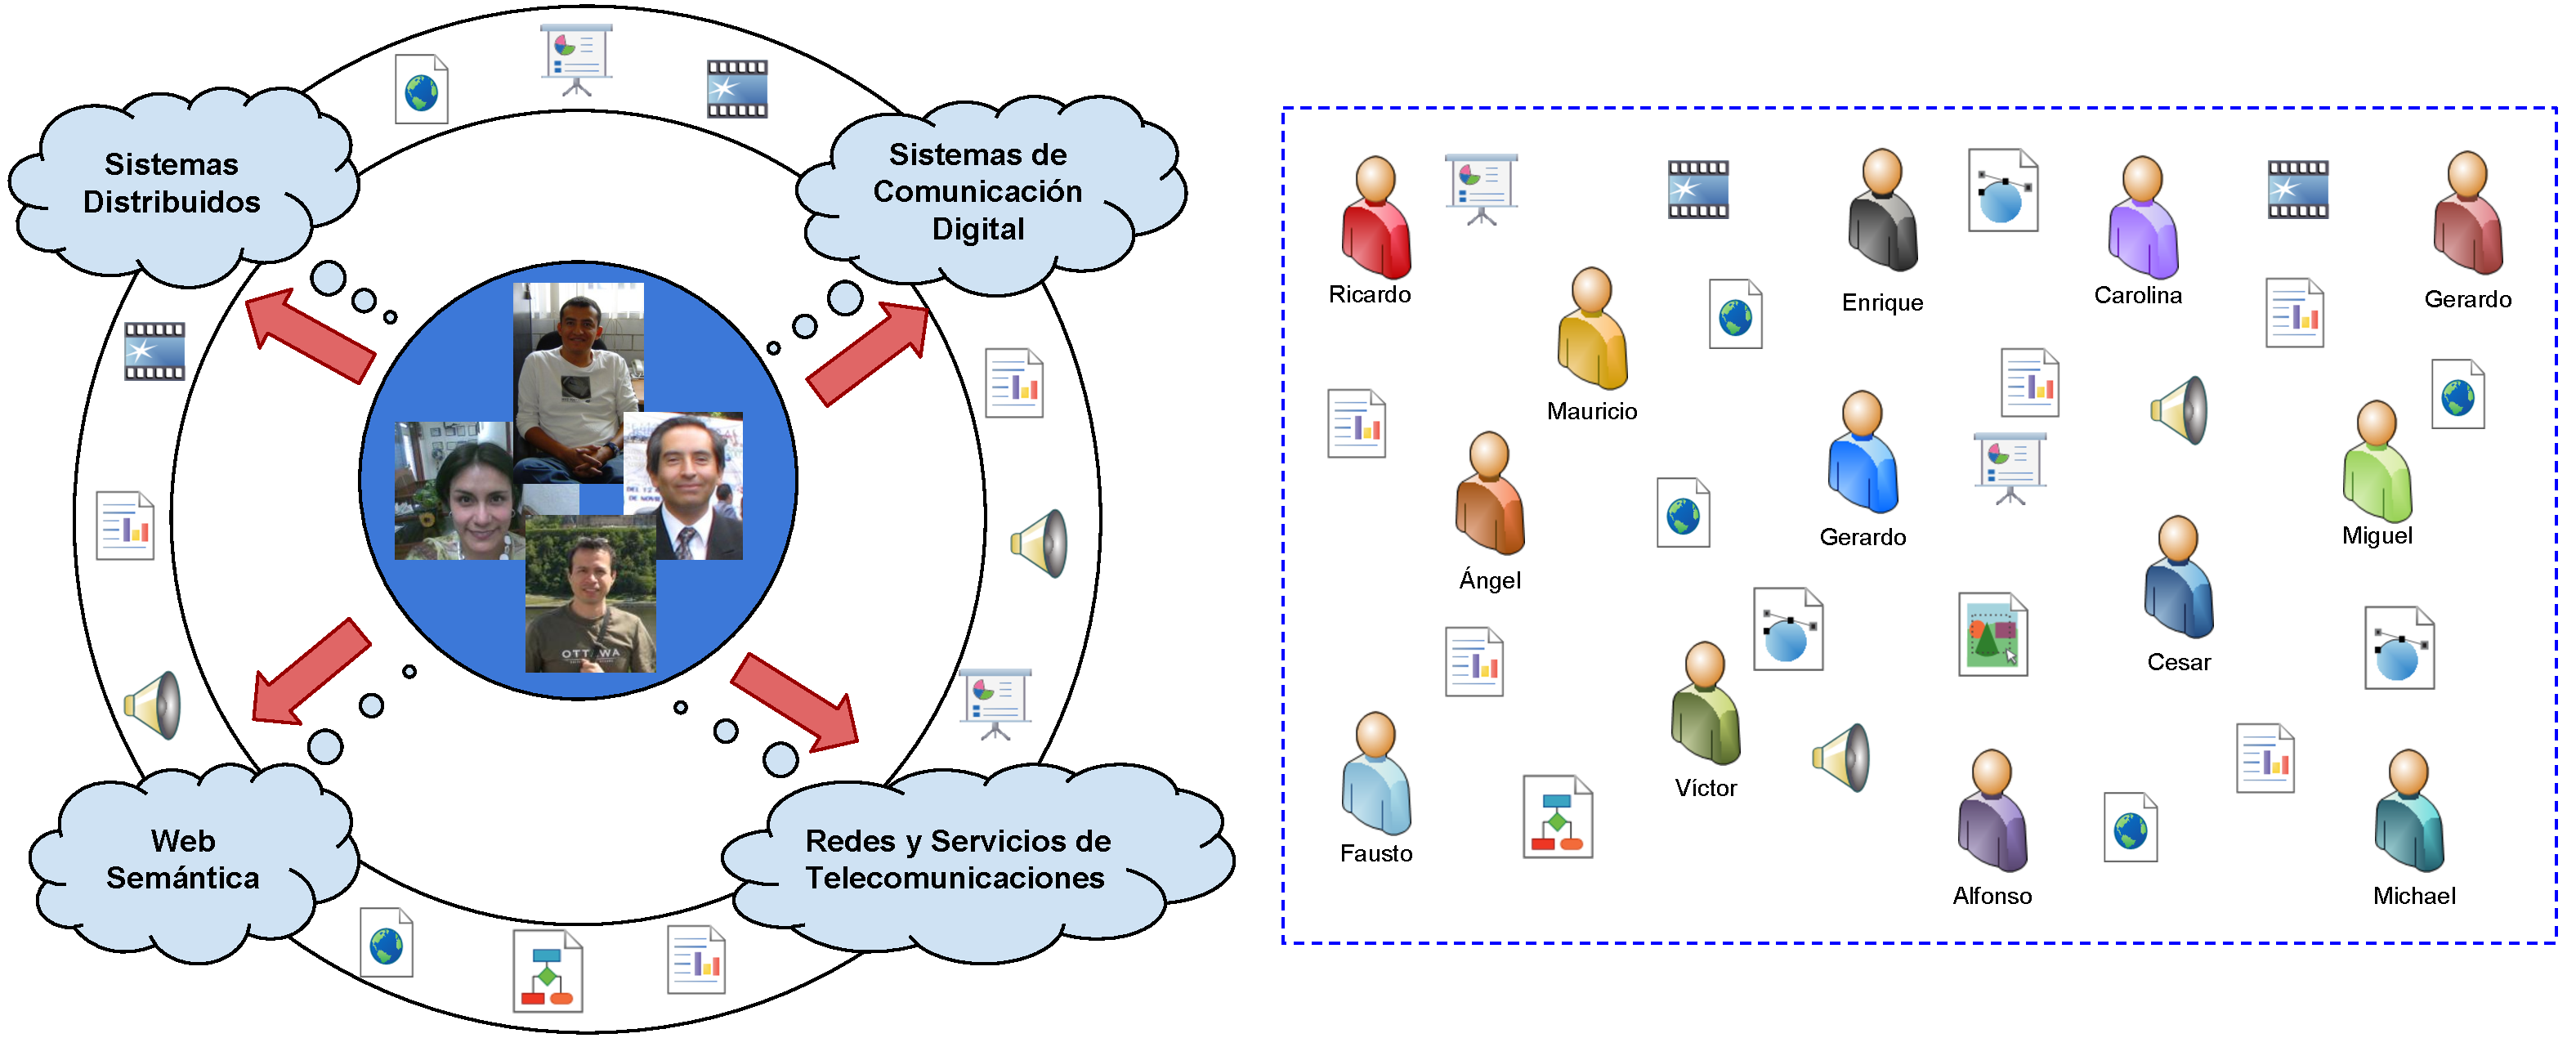
\includegraphics[width=0.7\textwidth]{CasosUsoMC}
\caption{Recursos de informaci�n agrupados por casos de uso para nuestra memoria corporativa.}
\label{fig:mccu}
\end{figure}



\section{Enriquecimiento del conocimiento en el modelo}
Hay que mostrar las jerarqu�as de clases y de propriedades, as� como los axiomas de nuestras ontolog�as.

Dado que los casos de uso son independientes, decidimos utilizar una ontolog�a para cada uno y otra que es de uso com�n (ODARyT).


\section{B�squeda y recuperaci�n de informaci�n en el modelo}
Aqu� hay que retomar nuestros casos de uso y expandirlos con consultas espec�ficas que se hacen sobre las ontolog�as definidas en la secci�n anterior.

Es importante hacer notar que ciertas consultas explotan a los axiomas, por lo que se requiere de un razonador.
\chapter{Prototipo}
\label{cap:piu}
%%No solo basta con un razonador también se requiere un modulo integrador de la información que transforme las consultas de los usuarios expresadas en lenguaje natural, a lenguaje que sea interpretado por el razonador. Además este integrador es el encargado de regresar los enlaces y los datos del recurso. De esta manera el motor de búsqueda queda de la siguiente manera:

%%Para llevar acabo está integración de la información es necesario un prototipo que satisfaga más eficientemente las consultas que escribe el usuario. De esta manera es necesario un análisis documental y técnico de los módulos de Anotaciones, Ontología de Dominio y Razonadores. Con la finalidad de tener una propuesta de sistema con las últimas novedades hechas en búsqueda y recuperación de la información basada en la semántica de los recursos.

%%se requiere proporcionar interfaces fáciles de usar, para simplificar a los miembros el proceso de generación de anotaciones y colocar en contexto su trabajo.  Un buen enfoque para un sistema de anotaciones es aquel donde se maneja una única interfaz, y es en esta donde los usuarios crean, modifican y comparten sus anotaciones.

%%La interfaz debe tener ..., para que los usuarios estructuren sus consulta, capturando los valores que desean buscar. En la interfaz debe proporcionar un navegador entre personas, documentos, multimedia, para que los usuarios que no tienen algún conocimiento previo de las personas y recursos digitales, puedan tener una vision general de la información de los recursos.

%%La interfaz debe permitir hacer las siguientes actividades a los usuarios:
%%•	Login.
%%•	Navegar entre personas.
%%o	Filtrar por ocupación.
%%o	Mostrar la información más detallada de una persona.
%%o	Búsqueda Avanzada de las personas.
%%•	Navegar entre documentos.
%%o	Filtrar por clase de documento.
%%o	Mostrar la información más detallada de un documento.
%%o	Búsqueda Avanzada de documentos.
%%•	Navegar entre multimedia.
%%o	Filtrar por clase multimedia.
%%o	Mostrar la información más detallada de un recurso multimedia.
%%o	Búsqueda Avanzada de recursos multimedia.
%%•	Búsqueda en todos los recursos de información por información semejante.

%%Las distintas aplicaciones que hay pueden ser elaboradas para Windows, Linux, Macs, u otros sistemas operativos, y también se pueden tener distintas versiones del mismo sistema para poder trabajar entre los distintos sistemas operativos. Lo ideal es que sin importar cual sea el sistema operativo el usuario pueda realizar sus anotaciones semánticas, para logara esto se puede emplear una aplicación web o aplicaciones elaboradas en java.
%%Si se emplea una aplicación web no es necesario instalar algún software extra, solo basta que el usuario acceda utilizando su navegador web de preferencia y comience el proceso de creación de anotaciones semánticas.

%%Por otro lado al usar una aplicación basada en Java, es necesario tener Java Development Kit (JDK) que es independiente de la plataforma, para tener un entorno amigable al usuario.

%%Finalmente, los usuarios necesitan una interfaz de usuario, para la consulta de información de las tripletas. Nosotros proponemos una interfaz amigable que sea accesible vía Web. De esta manera, los usuarios no instalan ningún componente y simplemente acceden a la página Web del sistema.
%%La interfaz al ser accesible vía Web, requiere ser instalada en un servidor Web. Para tomar la decisión sobre qué servidor es el apropiado para la interfaz. Nosotros debemos tomar en cuenta, el lenguaje de implementación del triplestore. Si el lenguaje es PHP9, entonces, podemos emplear un servidor HTTP Apache10. En otro caso, si el lenguaje es Java11 y permite implementar Servlet, entonces el servidor es Apache Tomcat12. 

\chapter{Evaluaci�n experimental}
\label{cap:exp}
%%%% Observaci�n consiste en la medida y registro de hechos observables.
La \textit{integraci�n sem�ntica de los recursos} es el proceso de b�squeda y recuperaci�n de informaci�n en un \textit{grafo de conocimiento (ontolog�a)}. Un \textit{motor de b�squeda de tripletas} es el mecanismo encargado de realizar la consulta de informaci�n en los grafos de conocimiento, para responder una consulta dada. Este \textit{motor de tripletas} generalmente pertenece a un triplestore. En esta tesis, se emplea el \textit{triplestore Jena}; las razones de la elecci�n de Jena son presentadas en la Secci�n \ref{sec:eoats}. Jena proporciona dos componentes importantes: 1) \textit{un motor de b�squeda} para tripletas RDF y 2) \textit{un motor de inferencia} que soporta los axiomas en nuestras ontolog�as, los cuales son descritos en la Secci�n \ref{sec:enrKrec}.

\section{Observaciones}
El \textit{n�mero de los resultados} depende del uso o no de inferencia en nuestros modelos sem�nticos. Si Jena no hace uso de \textit{inferencia}, como el ejemplo de la Figura \ref{fig:grafoSR}, entonces el \textit{motor de b�squeda} puede proporcionar todos, varios o ning�n resultado. Esta variedad en la entrega de resultados, depende de las consultas SPARQL: 1) \textit{consultas sobre las declaraciones de los recursos}, como la consulta de la Figura \ref{fig:q112rql}, 2) \textit{consultas que agrupan varios patrones para un criterio de b�squeda}, como las consultas de las Figuras \ref{fig:q2rqlSR} y \ref{fig:q2torqlSR}, y 3) \textit{consultas simplificadas}, como en las Figuras \ref{fig:q2rqlCR} y \ref{fig:q2torqlCR}. En contraste, si Jena emplea inferencia, entonces puede entregar mejores resultados completos con respecto a la ontolog�a. Un ejemplo de este modelo se presenta en la Figura \ref{fig:grafoCR}.

Una caracter�stica asociada al uso de inferencia, es el impacto en el \textit{tiempo de procesamiento} de \textit{Jena} para responder las consultas. Por un lado, se ha observado que el \textit{tiempo de consulta} de Jena es peque�o, menor a medio segundo, cuando usa un \textit{modelo sin inferencia}. Mientras, el \textit{tiempo de consulta} de Jena para un \textit{modelo con inferencia} es mayor en comparaci�n con el tiempo del \textit{modelo sin inferencia}.

%%%% Hip�tesis es una soluci�n para un problema dado.
\section{Hip�tesis}
Con base en estas observaciones, nuestras dos hip�tesis de experimentaci�n  son �stas:
\begin{enumerate}
\item La \textit{inferencia} es un proceso importarte para la consulta de informaci�n mediante un triplestore que soporte a �sta.
%\textit{El \textbf{triplestore Jena} obtiene \textbf{resultados completos con respecto a la ontolog�a} cuando utiliza nuestros modelos con inferencia}.
\item El proceso de inferencia implica mayores tiempo de consulta, pero �stos son aceptables con Jena.
%\textit{El \textbf{tiempo de consulta} de Jena es \textbf{mayor} para nuestros \textit{modelos con inferencia} en comparaci�n con nuestros \textbf{modelos sin inferencia}}.
\end{enumerate}

%%%% M�todo consiste en: la elecci�n de los sujetos para confirmar la muestra, el procedimiento a seguir para �stos, las variables consideradas: dependiente, independiente y auxiliares.

%%Elaborar un experimento que ponga a prueba una hip�tesis
\section{Experimentaci�n}
Esta experimentaci�n consiste en la realizaci�n de dos actividades para probar nuestras hip�tesis de experimentaci�n. \textit{La \textbf{primera actividad} es \textbf{evaluar la calidad de los resultados} de Jena para los modelos con y sin inferencia}. Esta evaluaci�n consiste en estas etapas: 1) establecer una serie de consultas para interrogar nuestros modelos, 2) encontrar manualmente cu�ntos y cu�les recursos responden las consultas, 3) ejecutar las consultas con el motor ARQ de Jena y 4) comparar los recursos dados por Jena con las respuestas manuales.

\textit{La \textbf{segunda actividad} consiste en medir los \textbf{tiempos promedio de procesamiento} de Jena para las consultas de nuestra primera actividad}. La finalidad de esta segunda actividad es comparar los \textit{tiempos de consulta} para un modelo con inferencia y otro que no emplea �sta. En ambos modelos se eval�a el tiempo desde \textit{la ejecuci�n de Jena para una consulta a un modelo (con o sin inferencia)} hasta \textit{la presentaci�n de los resultados en pantalla}.

%%La determinaci�n del tiempo para modelos sin inferencia, consiste en medir los tiempos de: 1) \textit{ejecuci�n de la consulta en en el modelo} y 2) \textit{recuperaci�n de la informaci�n}. De la misma manera, la medici�n de tiempos para un modelo con inferencia es parecida a la medici�n en un modelos sin inferencia. La excepci�n es que en un modelo con inferencia, se toman en cuenta los tiempos para: \textit{el proceso de inferencia en el modelo} y \textit{la ejecuci�n de la consulta al modelo inferido}.

En esta tesis, el proceso de \textit{integraci�n sem�ntica} est� asociado a dos \textit{casos de uso} (cartograf�a de competencias y b�squeda de recursos digitales). Ahora bien, nuestra experimentaci�n consiste en probar la \textit{calidad de los resultados} y el \textit{tiempo de procesamiento} para la \textit{integraci�n sem�ntica de recursos} en la \textit{memoria corporativa} del �rea de Redes y Telecomunicaciones. Por esta raz�n, las dos actividades de nuestra experimentaci�n deben ser aplicadas a nuestros dos \textit{casos de uso}.

%%Elecci�n de los sujetos para confirmar la muestra
\section{Sujetos de experimentaci�n}
\label{sec:subexp} 
Los sujetos de nuestra experimentaci�n son un conjunto de ontolog�as que consisten en personas, documentos y archivos multimedia que son generados artificialmente. Esta \textit{generaci�n artificial} consiste en el uso de scripts para: 1) \textit{asignar un identificador URI para un conjunto de \textbf{recursos de informaci�n ficticios}} y 2) \textit{generar tripletas RDF para estos recursos con base en las \textbf{propiedades} y \textbf{clases} de nuestras ontolog�as, as� como \textbf{datos aleatorios}}. 

Un script genera un conjunto de declaraciones para los recursos persona. Mientras, otro script genera las declaraciones para los documentos y archivo multimedia. El algoritmo \ref{alg:fsg} presenta el funcionamiento general de ambos scripts para la generaci�n y almacenamiento de tripletas RDF.

\begin{algorithm}
\SetKwData{Sigma}{$\sigma_i$}
\SetKwData{Model}{$modelo_{rdf}$}
$N\leftarrow$  n�mero de \textit{recursos ficticios de informaci�n} a describir\;
\Model$\leftarrow$Crear un modelo rdf\;
\For{$i\leftarrow 1$ \KwTo $N$}{
	\Sigma$\leftarrow$Crear el recurso $i$ y establecer un identificador URI para �ste\;
	Elaborar los valores para cada caracter�stica significativa de este recurso (\Sigma)\; \label{lin:values}
	Escribir las aserciones, concatenando el URI del recurso (\Sigma), las propiedades de la ontolog�a y los valores del paso \ref{lin:values}\;
}
Guardar el \Model en un archivo con extensi�n ``\textit{rdf}'' y sintaxis de serializaci�n \textit{Turtle}\;
\caption{Funcionamiento b�sico de scripts para la generaci�n de tripletas artificialmente.}
\label{alg:fsg} 
\end{algorithm}

El ap�ndice \ref{aped:AlgDS} presenta los dos algoritmos con el funcionamiento detallado de los scripts. Un algoritmo para los datos simulados de los recursos persona y el otro para los recursos digitales.

La finalidad del uso de \textit{informaci�n simulada} es tener r�pidamente un volumen grande de datos en nuestros ABoxes. La \textit{cantidad de informaci�n} en estos ABox debe ser realista con respecto al �rea de Redes y Telecomunicaciones (RyT). Ya que al tener informaci�n realista, nuestra experimentaci�n se ajusta a la cantidad de datos que esperamos manejar en la integraci�n sem�ntica. Otra raz�n del uso de informaci�n simulada es ver si Jena soporta esta escala realista de datos. Esta \textit{escala de datos} se obtiene a partir de la media de \textit{recursos digitales} que un profesor del �rea de RyT utiliza en un trimestre, as� como el n�mero promedio de profesores y alumnos que hay en esta �rea.

Las cantidades de \textit{recursos persona} son 60 recursos artificiales y 13 recursos reales, dando un total de 73 personas. Mientras, las cantidades para los \textit{recursos digitales} son 16 recursos reales y 1314 recurso simulados, un total de 1330 recursos digitales.

En nuestra experimentaci�n, algunos \textit{recursos persona} tienen la declaraci�n que los asignan expl�citamente a una de estas clases: \textit{Estudiante (sirp:Student)}, \textit{Empleado (sird:Employee)} y \textit{Profesor (sirp:Teacher)}. Otros recursos persona carecen de esta asignaci�n, pero con inferencia �stos pueden clasificarse en una o varias clases de la \textit{ontolog�a cartograf�a de competencias}. De esta manera, se ve el impacto de hacer razonamiento.

En concreto, se tienen estas \textit{cantidades de recursos} por clase: 51 recursos son profesionistas y 23 son \textit{estudiantes}. Los 51 recursos persona mediante inferencia son asignados a la clase \textit{Profesionista (sirp:Professional)}. De estos 51 profesionistas se tiene que 19 son profesores y 9 son empleados. Por otro lado, de los 23 estudiantes se tiene que 9 recursos est�n asignados a la clase \textit{Estudiante} y los 14 restantes por inferencia son asignados a la clase \textit{Estudiante}. Existen 13 recursos persona que mediante inferencia se clasifican en la clase \textit{Investigador (sirp:Researcher)}.

La Tabla \ref{tab:noRP} muestra las cantidades de \textit{recursos persona} por clases de la \textit{ontolog�a cartograf�a de competencias}. La \textit{primera columna} presenta el nombre de las clases, la \textit{segunda} el n�mero de recursos que tienen la declaraci�n que los asigna expl�citamente a una clase y la \textit{tercera columna} el n�mero de recursos que por inferencia tienen la declaraci�n para asignarlos a una clase.

\begin{table}[!htb]
\renewcommand{\arraystretch}{1.2}
\centering
\begin{tabular}{| >{\centering\arraybackslash}m{2in} | >{\centering\arraybackslash}m{1.5in} | >{\centering\arraybackslash}m{1.5in} | }
\hline 
\multirow{2}{*}{\textbf{Clase}} & \multicolumn{2}{c|}{\textbf{N�mero de Recursos}} \\
\cline{2-3} 
 & \textbf{Sin inferencia} & \textbf{Con inferencia}\\
\hline 
\hline
Persona & 0 & 73\\
\hline
Investigador & 0 & 13\\
\hline
Profesionista & 0 & 51\\
\hline
Estudiante & 11 & 23\\
\hline
Profesor & 19 & 19\\
\hline
Empleado & 9 & 9\\
\hline
\end{tabular}
\caption{N�mero de recursos persona por clase.}
\label{tab:noRP}
\end{table}

De la misma manera que los \textit{recursos persona}, algunos \textit{recursos digitales} tienen la declaraci�n que los asignan expl�citamente a una clase. Otros recursos carecen de esta asignaci�n, pero con inferencia �stos pueden clasificarse en una o varias clases de la \textit{ontolog�a b�squeda de recursos digitales}.

Los 1330 recursos digitales de nuestra experimentaci�n se clasifican en: 156 art�culos, 366 libros, 34 reportes t�cnicos, 146 p�ginas web, 73 tesis, 42 videos, 42 audios, 77 im�genes y 112 presentaciones. De los 156 art�culos, 89 recursos tienen la declaraci�n expl�cita a la clase \textit{Art�culo (sird:Paper)} y los restantes 67 mediante inferencia tienen la declaraci�n a esta clase. En los libros, 185 recursos tienen la declaraci�n expl�cita y 181 recursos mediante inferencia tienen la declaraci�n a la clase \textit{Libro (sird:Book)}. De la misma manera, 79 recursos tienen la declaraci�n expl�cita a la clase \textit{P�gina Web (sird:PageWeb)} y 31 recursos a la clase \textit{Tesis (sird:Thesis)}. Mientras, 67 recursos mediante inferencia pertenecen a la clase  \textit{P�gina Web} y 42 a la clase \textit{Tesis}. Por �ltimo, los 1330 recursos se clasifican en 815 \textit{Documentos (sird:Document)} y 515 \textit{Multimedia (sird:Multimedia)}. Las declaraciones a estas dos clases se obtienen mediante inferencia.

La Tabla \ref{tab:noRD} presenta las cantidades de recursos digitales por clases de la \textit{ontolog�a recursos digitales}. Esta Tabla \ref{tab:noRD} presenta la misma estructura de la Tabla \ref{tab:noRP}.

\begin{table}[!htb]
\renewcommand{\arraystretch}{1.1}
\centering
\begin{tabular}{| >{\centering\arraybackslash}m{2in} | >{\centering\arraybackslash}m{1.5in} | >{\centering\arraybackslash}m{1.5in} | }
\hline 
\multirow{2}{*}{\textbf{Clase}} & \multicolumn{2}{c|}{\textbf{N�mero de Recursos}} \\
\cline{2-3} 
 & \textbf{Sin inferencia} & \textbf{Con inferencia}\\
\hline 
\hline
Recurso Digital & 0 & 1330\\
\hline
Documento & 0 & 815\\
\hline
Art�culo & 89 & 156\\
\hline
Reporte T�cnico & 34 & 34\\
\hline
P�gina Web & 79 & 146\\
\hline
Tesis & 31 & 73\\
\hline
Libro & 185 & 366\\
\hline
Multimedia & 0 & 515\\
\hline
Presentaci�n & 112 & 112\\
\hline
Audio & 42 & 42\\
\hline
V�deo & 42 & 42\\
\hline
Imagen & 77 & 77\\
\hline
\end{tabular}
\caption{N�mero de recursos digitales por clase.}
\label{tab:noRD}
\end{table}

\section{Metodolog�a}
Esta experimentaci�n se ha dividido en dos actividades. La primera actividad consiste en la \textit{evaluaci�n de la calidad de los resultados} que proporciona el triplestore Jena. Mientras, la segunda actividad consiste en medir los \textit{tiempos promedios} que toma Jena para: consultar los modelos con/sin inferencia y mostrar los resultados al usuario.

El \textit{primer paso} en la \textit{evaluaci�n de la calidad de resultados} es identificar un conjunto b�sico de consultas para interrogar las ontolog�as \textit{cartograf�a de competencias} y \textit{b�squeda de recursos digitales}. En la Secci�n \ref{sec:byrKrec} se hizo un an�lisis e identificaci�n de preguntas base que posteriormente se transformaron a consultas SPARQL. Estas consultas de la Secci�n \ref{sec:byrKrec} son reutilizadas para la primer actividad de esta experimentaci�n.

El \textit{segundo paso} es encontrar cu�ntos y cu�les recursos son relevantes para responder las consultas de nuestra experimentaci�n. Para ello, se hace una \textit{b�squeda manual} exhaustiva de los recursos relevantes que responden las consultas de experimentaci�n. Esta b�squeda se hace sobre los recursos de nuestra memoria corporativa que est� guiada por los casos de uso. Para cada consulta, se anotan los identificadores URI de los \textit{recursos relevantes} y la cantidad de �stos.

La Tabla \ref{tab:qrynoRP} muestra las preguntas base para la \textit{cartograf�a de competencias}. En esta Tabla, la primera columna presenta el identificador para cada una de las diecinueve preguntas, la segunda columna enuncia la pregunta y la tercer columna presenta el n�mero de recursos que responden a �sta. De la misma manera, la Tabla \ref{tab:qrynoRD} presenta un identificador, las preguntas y cantidad de recursos que responden a �stas, para la \textit{b�squeda de recursos digitales}. En estas dos Tablas, no se presentan los identificadores URI de los recursos que responden a las preguntas, porque algunas consultas tienen muchos recursos relevantes.

\begin{table}[!hp]
\renewcommand{\arraystretch}{1.4}
\centering
\begin{tabular}{>{\centering\arraybackslash}m{1in} >{\arraybackslash}m{3.5in} >{\centering\arraybackslash}m{1in}}
\hline 
Id. Consulta & Pregunta & No. de Recursos\\
\hline
\hline 
Q1.1 &  �Cu�les el nombre, correo, sitio web, g�nero y edad de las personas del �rea de RyT? & 73 \\
\hline
Q1.2 & �Cu�l es el nombre, sitio web y el lugar donde laboran las personas del RyT? & 73\\
\hline 
Q1.3 & �Qui�nes son mayores de 20 a�os y menores de 45 a�os? & 50\\
\hline 
Q1.4 & �Qui�nes son profesionistas del �rea de RyT? & 51\\
\hline 
Q1.5 & �Qui�nes trabajan en Clark \& Parsia y son del sexo Masculino? & 3\\
\hline 
Q1.6 & �Qui�nes son estudiantes y leen en ingl�s? & 8\\
\hline 
Q1.7 & �Quienes hablan, leen y escriben en ingl�s? & 16\\
\hline 
Q1.8 & �Qu� estudiantes saben algo de ingl�s? & 6\\
\hline 
Q1.9 & �Qu� profesores tienen la capacidad de s�ntesis? & 2\\
\hline 
Q1.10 & �Qu� profesionistas tienen conocimiento en los temas de Web Sem�ntica? & 58\\
\hline
Q1.11 & �Qu� profesores tienen conocimientos en Sistemas Distribuidos? & 3\\
\hline 
Q1.12 & �Qui�nes tienen conocimiento en Java, OWL, RDF, Threads, C, OpenMP? & 1\\
\hline 
Q1.13 & �Qu� estudiantes tienen alg�n conocimiento en los subtemas de Sistemas Operativos? & 33\\
\hline 
Q1.14 & �Qui�nes trabajan en una Universidad? & 24\\
\hline 
Q1.15 & �Quienes laboran en la UAM y tienen alg�n conocimiento en  Web Sem�ntica? & 19\\
\hline 
Q1.16 & �Qu� personas tienen como asesor a Carolina Medina? & 2\\
\hline 
Q1.17 & �Qui�nes son los colegas de Ricardo Marcelin? & 8\\
\hline 
Q1.18 &  �Qui�nes conocen a Carolina Medina Ramirez? & 11\\
\hline 
Q1.19 & �Qu� personas son profesores-investigadores? & 9\\
\hline 
\end{tabular}
\caption{Preguntas y cantidad de personas que responden a �stas.}
\label{tab:qrynoRP}
\end{table}

\begin{table}[!hp]
\renewcommand{\arraystretch}{1.4}
\centering
\begin{tabular}{>{\centering\arraybackslash}m{1in} >{\arraybackslash}m{3.5in} >{\centering\arraybackslash}m{1in}}
\hline 
Id. Consulta & Pregunta & No. de Recursos\\
\hline
\hline 
Q2.1 & �Cu�les son los t�tulos, rutas, extensi�n, idioma de todos los recursos digitales de RyT? & 1330 \\
\hline
Q2.2 & �Cu�les libros tratan sobre algunos temas de Sistemas Distribuidos? & 103\\
\hline 
Q2.3 & �Qu� recursos fueron publicados por la UAM? & 18\\
\hline 
Q2.4 & �Qu� documentos son para dar un curso de Sistemas P2P? & 31\\
\hline 
Q2.5 & �Qu� recursos multimedia son mayores al a�o 2009? & 119\\
\hline 
Q2.6 & �Cu�les documentos tratan sobre Ontolog�as? & 30\\
\hline 
Q2.7 & �Qu� recursos fueron publicados en una Revista cient�fica? & 156\\
\hline 
Q2.8 & �Qu� recursos tienen en su contenido las palabras "linked data"? & 159\\
\hline 
Q2.9 & �Cu�les documentos en ingl�s y mayores al a�o 2000 son de autor�a de Erik Alarc�n Zamora? & 2\\
\hline 
Q2.10 & �Cu�les la tesis de Samuel Hern�ndez Maza? & 4\\
\hline 
\end{tabular}
\caption{Preguntas y cantidad de recursos digitales que responden a �stas.}
\label{tab:qrynoRD}
\end{table}

En el Anexo \ref{aped:TrPC}, se presentan las consultas SPARQL que est�n asociadas a cada pregunta de las Tablas \ref{tab:qrynoRP} y \ref{tab:qrynoRD}.

El \textit{tercer paso} es emplear \textit{Jena} para ejecutar las \textit{consultas SPARQL} a un modelo sin inferencia y otro con inferencia. La finalidad de esto es ver la calidad de resultados y la cantidad de �stos que al emplear un modelo con inferencia y otro sin inferencia. De esta manera, podemos ver el impacto de la inferencia para la consulta de informaci�n en una ontolog�a.

En esta \textit{ejecuci�n de consultas}, se emplea un script para consultar un \textit{modelo sem�ntico} y proporcionar los resultados que est�n asociados a una consulta dada. El funcionamiento de este script se presenta en el Algoritmo \ref{alg:srinf}. En este algoritmo, los \textbf{\textit{par�metros de entrada}} son: 1) \textit{la consulta SPARQL}, 2) \textit{la ontolog�a} (\textit{Personas o RecDigi}), 3) \textit{inferencia} (\textit{0 sin inferencia} y \textit{1 con inferencia}). Mientras, los par�metros de salida son: 1) \textit{los identificadores URI que responden la consulta} y 2) \textit{la cantidad de recursos respuesta}. Este script permite ejecutar una consulta a la vez por corrida e imprime los par�metros de salida en pantalla.

\begin{algorithm}
\SetKwData{Model}{$modelo_{semantico}$}
\KwIn{Consulta SPARQL: $query$, Nombre del modelo: $model$, Uso de inferencia: $inference$}
\KwOut{Resultados: $\Pi_{query}$, N�mero de resultados: $noRes$}
\BlankLine
$noRes \leftarrow 0, \Pi_{query} \leftarrow \{ \}$\;
\uIf{$model \equiv$ `Personas'}{
	Cargar en memoria el ABox y TBox de la ontolog�a cartograf�a de competencias\;
}
\ElseIf{$model \equiv$ `RecDigi'}{
	Cargar en memoria el ABox y TBox de la ontolog�a b�squeda de recursos digitales\;
}
\uIf{$inference \equiv 0$}{
	\Model $\leftarrow$ modelo ABox y TBox\;
}
\ElseIf{$inference \equiv 1$}{
	Inferir en memoria sobre el ABox y TBox\;
	\Model $\leftarrow$ modelo inferido\;
}
Cargar en memoria consulta SPARQL ($query$)\;
Ejecutar consulta ($query$) en el modelo (\Model)\;
$\Pi_{query} \leftarrow$ Recuperar resultados de consulta\tcc*{$\Pi_{query} = \{ \pi_1, \dots, \pi_n \}$}
\ForAll{elements of $\Pi_{query}$}{
	Imprimir $\pi_k$ en pantalla\;
	$noRes \leftarrow noRes + 1$\;
}
Imprimir $noRes$ en pantalla\;
\caption{Algoritmo para la evaluaci�n de la calidad de resultados}
\label{alg:srinf} 
\end{algorithm}

El \textit{cuarto paso} es comparar los \textit{resultados que proporciona el script (Algoritmo \ref{alg:srinf})} con los \textit{resultados que sabemos responden (b�squeda manual)} las consultas de las Tablas \ref{tab:qrynoRP} y \ref{tab:qrynoRD}. La finalidad de este paso, es \textit{evaluar} la calidad de resultados de Jena, para un modelo con inferencia y otro sin el uso de �sta. El cuarto paso, se hace en dos fases: 1) \textit{encontrar los recursos relevantes} de las respuestas dadas por el script, y 2) usar (\textit{m�tricas de recuperaci�n de la informaci�n}) para comparar la calidad de los resultados con y sin inferencia. 

La \textit{fase uno} consiste en comparar y anotar las cantidades de recursos relevantes para cada consulta. En esta fase se considera el modelo de uso: con inferencia o sin �sta. Esta comparaci�n y anotaci�n se hizo de forma manual. El primer criterio de comparaci�n es ver la cantidad de recursos de las Tablas \ref{tab:qrynoRP} y \ref{tab:qrynoRD} con el n�mero de respuestas que proporciona el script. Posteriormente, se hace la comparaci�n \textit{identificador} a \textit{identificador} de \textit{los recursos que son proporcionados por el script} con \textit{los recursos que se saben responden a la consulta}.

La segunda fase, consiste en emplear dos m�tricas de \textit{recuperaci�n de la informaci�n (RI\label{sym:ri})}:

\begin{itemize}
\item La \textbf{\textit{exhaustividad (recall)}} \cite{Nasraoui} es ``\textit{la cantidad de elementos relevantes que han sido recuperados, entre la cantidad de elementos relevantes en la base de conocimientos}'' \cite{RecYPres}. La exhaustividad se presenta en la Ecuaci�n \ref{ec:exa}.

\begin{equation}
	Exhaustividad = \frac{N\acute{u}mero\: de\: recursos\: relevantes\: que\: han\: sido\: recuperados}{N\acute{u}mero\: de\: recursos\: relevantes\: en\: la\: base\: de\: conocimientos} * 1.0
	\label{ec:exa}
\end{equation}

\end{itemize}

\begin{itemize}
\item La \textbf{\textit{precisi�n (precision)}} \cite{Nasraoui} es la ``\textit{cantidad de elementos recuperados que son relevantes, entre el total de elementos recuperados}'' \cite{RecYPres}. La precisi�n se presenta en la Ecuaci�n \ref{ec:pre}.

\begin{equation}
	Precisi�n = \frac{N\acute{u}mero\: de\: elementos\: relevantes\: que\: han\: sido\: recuperados}{Total\: de\:elementos\: recuperados\: en\: la\: base\: de\: conocimientos} *1.0
	\label{ec:pre}
\end{equation}
\end{itemize}

En las ecuaciones de la exhaustividad y precisi�n, los divisores y dividendos son elementos que se han encontrado en esta primer actividad. En concreto, �stos son los elementos en las dos ecuaciones:

\begin{itemize}
\item \textit{Exhaustividad}: La \textit{cantidad de elementos relevantes recuperados} es el \textit{n�mero de recursos relevantes que proporciona el script para una consulta}; esta informaci�n se obtiene en el etapa uno de este cuarto paso. Mientras, el n�mero de \textit{elementos relevantes en la base de conocimiento} es la \textit{cantidad de resultados de nuestra b�squeda manual} que est�n en las Tablas \ref{tab:qrynoRP} y \ref{tab:qrynoRD}.
\item \textit{Precisi�n}: La \textit{cantidad de elementos relevantes recuperados} es el \textit{n�mero de recursos relevantes que proporciona el script para una consulta}. Mientras, \textit{el total de elementos recuperados en la base de conocimiento} es la cantidad de \textit{recursos dados por el script, sin el an�lisis de los recursos relevantes}.
\end{itemize}

El objetivo de emplear estas dos m�tricas, es evaluar las capacidades de \textit{recuperaci�n de la informaci�n} del triplestores Jena. En particular, la \textit{exhaustividad} eval�a la habilidad de Jena para encontrar los recursos relevantes en una ontolog�a, mientras la \textit{precisi�n} eval�a la habilidad de Jena para filtrar los recursos relevantes \cite{Cleverdon68}.

En esta experimentaci�n, la \textbf{segunda actividad} es tomar los tiempos de procesamiento para la consulta y recuperaci�n de informaci�n en un modelo sem�ntico a partir del uso de Jena. El objetivo de esta actividad es comparar estos tiempos de consulta para un modelo con inferencia y otro sin el uso de �sta.

Los tiempos importantes en esta actividad son la medici�n desde \textit{la consulta de informaci�n en un modelo sem�ntico con Jena} hasta \textit{la impresi�n de los resultados en pantalla}. Esta medici�n de los tiempos, se hace con base en la modificaci�n del script del Algoritmo \ref{alg:srinf}. Porque este Algoritmo \ref{alg:srinf} lleva a cabo todo el proceso de b�squeda y recuperaci�n de la informaci�n relevante en los \textit{recursos de informaci�n}. Tambi�n, este Algoritmo permite elegir el modelo: si es cero, entonces no hay inferencia y si es uno, se emplea inferencia.

El funcionamiento del \textit{script modificado} es tomar `\textbf{\textit{n}}' veces el \textit{tiempo de procesamiento} cuando se consulta un modelo sem�ntico (con o sin inferencia). Posteriormente, este script calcula y regresa el \textit{tiempo promedio de consulta} para una \textit{consulta SPARQL} dada. El Algoritmo \ref{alg:mod} presenta el funcionamiento de este script modificado.

\begin{algorithm}
\SetKwData{Model}{$modelo_{semantico}$}
\SetKwFunction{time}{time}
\KwIn{Consulta SPARQL: $query$, Nombre del modelo: $model$, Uso de inferencia: $inference$, N�mero de repeticiones: $N$}
\KwOut{Tiempo promedio: $Tiempo_{promedio}$}
\BlankLine
$\Pi_{query} \leftarrow \{ \}$\;
$t_{ini} \leftarrow 0, t_{fin} \leftarrow 0, Tiempo_{promedio} \leftarrow 0$\;
\For{$i\leftarrow 1$ \KwTo $N$}{
	\uIf{$model \equiv$ `Personas'}{
		Cargar en memoria el ABox y TBox de la ontolog�a cartograf�a de competencias\;
	}
	\ElseIf{$model \equiv$ `RecDigi'}{
		Cargar en memoria el ABox y TBox de la ontolog�a b�squeda de recursos digitales\;
	}
	\uIf{$inference \equiv 0$}{
		\Model $\leftarrow$ modelo ABox y TBox\;
	}
	\ElseIf{$inference \equiv 1$}{
		Inferir en memoria sobre el ABox y Tbox\;
		\Model $\leftarrow$ modelo inferido\;
	}
	Cargar en memoria consulta SPARQL ($query$)\;
	
	$t_{ini} \leftarrow$ \time{}\;
	Ejecutar consulta ($query$) en el modelo (\Model)\;
	$\Pi_{query} \leftarrow$ Recuperar resultados de consulta\tcc*{$\Pi_{query} = \{ \pi_1, \dots, \pi_n \}$}
	\ForAll{elements of $\Pi_{query}$}{
		Imprimir $\pi_k$ en pantalla\;
	}
	$t_{fin} \leftarrow$ \time{}\;
	$Tiempo_{promedio} \leftarrow Tiempo_{promedio} + (t_{fin} - t_{ini})$\;
}
\Return $Tiempo_{promedio}$\;
\caption{Algoritmo para medir el tiempo promedio en el proceso de consulta.}
\label{alg:mod} 
\end{algorithm}

%consiste en medir los \textbf{tiempos promedio de procesamiento} de Jena para las consultas de nuestra primera actividad}. La finalidad de esta segunda actividad es comparar los \textit{tiempos de consulta} para un modelo con inferencia y otro que no emplea �sta. En ambos modelos se eval�a el tiempo desde \textit{la ejecuci�n de Jena para una consulta a un modelo } hasta \textit{la presentaci�n de los resultados en pantalla}.

Este script (Algoritmo \ref{alg:mod}) se ejecuta para cada una de las consultas que est�n asociadas a las preguntas en las Tablas \ref{tab:qrynoRP} y \ref{tab:qrynoRD}. Porque, este script permite procesar una consulta a la vez. El n�mero de repeticiones se establece en 20 ($N = 20$). Mientras, las modelos empleados son las ontolog�as de \textit{cartograf�a de competencias} y \textit{b�squeda de recursos digitales}. El par�metro importante es el uso o no de inferencia para el modelo sem�ntico.

Los scripts asociados a los Algoritmos \ref{alg:srinf} y \ref{alg:mod}, se corrieron en una computadora con un procesador Intel Core I7 a 2.3GHz con 8Gb en RAM y 8 n�cleos de procesamiento. La versi�n del Apache Jena es la 2.7.4 para Windows 7 (64bits). Estos scripts se construyeron con el IDE Eclipse y se ejecutaron con la versi�n 1.7.0\_05 de Java.

\section{Resultados}
Los resultados para la \textit{evaluaci�n de la calidad de los resultados} se presentan en dos etapas. Estas dos etapas tienen relaci�n con las dos fases del cuarto paso de esta evaluaci�n. La primera etapa presenta la cantidad de resultados (relevantes y el total) que fueron recuperados por el script del Algoritmo \ref{alg:srinf}. La segunda etapa presenta los valores calculados para la exhaustividad y precisi�n. Este c�lculo se hace para cada consulta de la experimentaci�n.

\begin{table}[!htb]
\renewcommand{\arraystretch}{0.92}
\centering
\begin{tabular}{| >{\centering\arraybackslash}m{1in} | >{\centering\arraybackslash}m{1in} | >{\centering\arraybackslash}m{1in} | >{\centering\arraybackslash}m{1in} | >{\centering\arraybackslash}m{1in} | }
\hline 
\multirow{2}{*}{\textbf{Id. Consulta}} & \multicolumn{2}{c|}{\textbf{Modelo sin inferencia}} & \multicolumn{2}{c|}{\textbf{Modelo con inferencia}}\\
\cline{2-5} 
 & \textbf{Recursos relevantes} & \textbf{Total recursos recuperados} & \textbf{Recursos relevantes} & \textbf{Total recursos recuperados}\\
\hline 
\hline
Q1.1 & 73 & 73 & 73 & 73\\
\hline
Q1.2 & 73 & 73 & 73 & 73\\
\hline
Q1.3 & 50 & 50 & 50 & 50\\
\hline
Q1.4 & 28 & 28 & 51 & 51\\
\hline
Q1.5 & 3 & 3 & 3 & 3\\
\hline
Q1.6 & 4 & 4 & 8 & 8\\
\hline
Q1.7 & 16 & 16 & 16 & 16\\
\hline
Q1.8 & 2 & 2 & 6 & 6\\
\hline
Q1.9 & 10 & 10 & 10 & 10\\
\hline
Q1.10 & 2 & 2 & 58 & 58\\
\hline
Q1.11 & 3 & 3 & 3 & 3\\
\hline
Q1.12 & 1 & 1 & 1 & 1\\
\hline
Q1.13 & 6 & 6 & 20 & 20\\
\hline
Q1.14 & 16 & 16 & 24 & 24\\
\hline
Q1.15 & 2 & 2 & 2 & 2\\
\hline
Q1.16 & 2 & 2 & 2 & 2\\
\hline
Q1.17 & 2 & 2 & 8 & 8\\
\hline
Q1.18 & 7 & 7 & 11 & 11\\
\hline
Q1.19 & 0 & 0 & 13 & 13\\
\hline
\end{tabular}
\caption{Recursos relevantes y no relevantes asociados a las preguntas de la cartograf�a de competencias.}
\label{tab:rrRP}
\end{table}

En la Tabla \ref{tab:rrRP} se presentan las cantidades de recursos relevantes y totales de la primera etapa, para las preguntas de la Tabla \ref{tab:qrynoRP}. La primer columna presenta el identificador de consulta. La segunda y tercera columna muestra la cantidad de recursos relevantes y total recursos recuperados cuando se emplea un modelo sin inferencia. La cuarta y quinta presentan los recursos relevantes y total de recursos recuperados para un modelo con inferencia.

De la misma manera, la Tabla \ref{tab:rrRD} presenta la cantidad de recursos relevantes y total de recursos recuperados cuando se consulta el modelo sin inferencia y con inferencia de los recursos digitales. En esta Tabla, las consultas est�n asociadas a las preguntas de la Tabla \ref{tab:qrynoRD}. La estructura de la Tabla \ref{tab:rrRD} es igual a la Tabla \ref{tab:rrRP}.

\begin{table}[!htb]
\renewcommand{\arraystretch}{0.94}
\centering
\begin{tabular}{| >{\centering\arraybackslash}m{1in} | >{\centering\arraybackslash}m{1in} | >{\centering\arraybackslash}m{1in} | >{\centering\arraybackslash}m{1in} | >{\centering\arraybackslash}m{1in} | }
\hline 
\multirow{2}{*}{\textbf{Id. Consulta}} & \multicolumn{2}{c|}{\textbf{Modelo sin inferencia}} & \multicolumn{2}{c|}{\textbf{Modelo con inferencia}}\\
\cline{2-5} 
 & \textbf{Recursos relevantes} & \textbf{Total recursos recuperados} & \textbf{Recursos relevantes} & \textbf{Total recursos recuperados}\\
\hline 
\hline
Q2.1 & 1330 & 1330 & 1330 & 1330\\
\hline
Q2.2 & 0 & 0 & 103 & 103\\
\hline
Q2.3 & 18 & 18 & 18 & 18\\
\hline
Q2.4 & 15 & 15 & 31 & 31\\
\hline
Q2.5 & 66 & 66 & 119 & 119\\
\hline
Q2.6 & 15 & 15 & 30 & 30\\
\hline
Q2.7 & 156 & 156 & 156 & 156\\
\hline
Q2.8 & 159 & 159 & 159 & 159\\
\hline
Q2.9 & 0 & 0 & 2 & 2\\
\hline
Q2.10 & 3 & 3 & 4 & 4\\
\hline
\end{tabular}
\caption{Recursos relevantes y no relevantes asociados a las preguntas de la b�squeda de recursos digitales.}
\label{tab:rrRD}
\end{table}

Los resultados para la segunda etapa de la \textit{evaluaci�n de la calidad de resultados}, son los valores que fueron calculados para la exhaustividad (Ecuaci�n \ref{ec:exa}) y precisi�n (Ecuaciones \ref{ec:pre}) de Jena con nuestras ontolog�as. El objetivo de esta \textit{segunda etapa} es comparar estas dos m�tricas de \textit{recuperaci�n de la informaci�n} para un modelo con inferencia y otro que no usa �sta, donde estos modelos son procesados por Jena.

La Tabla \ref{tab:exprRP} muestra los valores de exhaustividad y precisi�n para las consultas en la Tabla \ref{tab:qrynoRP}. En esta Tabla \ref{tab:exprRP}, la primer columna muestra el identificador de la consulta. La segunda y tercera columna muestran los valores de exhaustividad y precisi�n para un modelo sin inferencia. La cuarta y quinta columna presentan los valores de las mismas m�tricas para un modelo con inferencia.

\begin{table}[!htb]
\renewcommand{\arraystretch}{0.92}
\centering
\begin{tabular}{| >{\centering\arraybackslash}m{1in} | >{\centering\arraybackslash}m{1.2in} | >{\centering\arraybackslash}m{1in} | >{\centering\arraybackslash}m{1.2in} | >{\centering\arraybackslash}m{1in} | }
\hline 
\multirow{2}{*}{\textbf{Id. Consulta}} & \multicolumn{2}{c|}{\textbf{Modelo sin inferencia}} & \multicolumn{2}{c|}{\textbf{Modelo con inferencia}}\\
\cline{2-5} 
 & \textbf{Exhaustividad} & \textbf{Precisi�n} & \textbf{Exhaustividad} & \textbf{Precisi�n}\\
\hline 
\hline
Q1.1 & 1 & 1 & 1 & 1\\
\hline 
Q1.2 & 1 & 1 & 1 & 1\\
\hline 
Q1.3 & 1 & 1 & 1 & 1\\
\hline 
Q1.4 & 0.549 & 1 & 1 & 1\\
\hline 
Q1.5 & 1 & 1 & 1 & 1\\
\hline 
Q1.6 & 0.5 & 1 & 1 & 1\\
\hline 
Q1.7 & 1 & 1 & 1 & 1\\
\hline 
Q1.8 & 0.333 & 1 & 1 & 1\\
\hline 
Q1.9 & 1 & 1 & 1 & 1\\
\hline 
Q1.10 & 0.034 & 1 & 1 & 1\\
\hline 
Q1.11 & 1 & 1 & 1 & 1\\
\hline 
Q1.12 & 1 & 1 & 1 & 1\\
\hline 
Q1.13 & 0.3 & 1 & 1 & 1\\
\hline 
Q1.14 & 0.666 & 1 & 1 & 1\\
\hline 
Q1.15 & 1 & 1 & 1 & 1\\
\hline 
Q1.16 & 1 & 1 & 1 & 1\\
\hline 
Q1.17 & 0.25 & 1 & 1 & 1\\
\hline 
Q1.18 & 0.636 & 1 & 1 & 1\\
\hline 
Q1.19 & 0 & - & 1 & 1\\
\hline
\end{tabular}
\caption{Exhaustividad y precisi�n para las consultas de la cartograf�a de competencias.}
\label{tab:exprRP}
\end{table}

De la misma manera, la Tabla \ref{tab:exprRD} presenta los valores de estas dos m�tricas de RI, para las preguntas de la Tabla \ref{tab:qrynoRD}. Estos valores est�n asociados al modelo de \textit{b�squeda de recursos digitales}. La estructura de esta Tabla \ref{tab:exprRD} es la misma de la Tabla \ref{tab:exprRP}.

\begin{table}[!htb]
\renewcommand{\arraystretch}{0.92}
\centering
\begin{tabular}{| >{\centering\arraybackslash}m{1in} | >{\centering\arraybackslash}m{1.2in} | >{\centering\arraybackslash}m{1in} | >{\centering\arraybackslash}m{1.2in} | >{\centering\arraybackslash}m{1in} | }
\hline 
\multirow{2}{*}{\textbf{Id. Consulta}} & \multicolumn{2}{c|}{\textbf{Modelo sin inferencia}} & \multicolumn{2}{c|}{\textbf{Modelo con inferencia}}\\
\cline{2-5} 
 & \textbf{Exhaustividad} & \textbf{Precisi�n} & \textbf{Exhaustividad} & \textbf{Precisi�n}\\
\hline 
\hline
Q2.1 & 1 & 1 & 1 & 1\\
\hline 
Q2.2 & 0 & - & 1 & 1\\
\hline 
Q2.3 & 1 & 1 & 1 & 1\\
\hline 
Q2.4 & 0.484 & 1 & 1 & 1\\
\hline 
Q2.5 & 0.555 & 1 & 1 & 1\\
\hline 
Q2.6 & 0.5 & 1 & 1 & 1\\
\hline 
Q2.7 & 1 & 1 & 1 & 1\\
\hline 
Q2.8 & 1 & 1 & 1 & 1\\
\hline 
Q2.9 & 0 & - & 1 & 1\\
\hline 
Q2.10 & 0.75 & 1 & 1 & 1\\
\hline
\end{tabular}
\caption{Exhaustividad y precisi�n para las consultas de la b�squeda de recursos digitales.}
\label{tab:exprRD}
\end{table}

Las Tablas \ref{tab:tiempRP} y \ref{tab:tiempRD} presentan los resultados de \textit{evaluar los tiempos promedio de procesamiento}. La Tabla Tablas \ref{tab:tiempRP} muestra los tiempos promedio de consulta para las preguntas en la Tabla \ref{tab:qrynoRP}. De la misma manera, la Tabla \ref{tab:tiempRD} muestra los tiempos para las preguntas en la Tabla \ref{tab:qrynoRD}. El objetivo de esta evaluaci�n es comparar los tiempos al consultar un modelo sin inferencia y otro con inferencia.

La estructura es la misma para las Tablas \ref{tab:tiempRP} y \ref{tab:tiempRD}. �sta es la estructura de estas Tablas: la primer columna muestra el identificador de la consulta, la segunda el tiempo promedio al consultar un modelo sin inferencia y la tercer columna el tiempo promedio de consulta en un modelo obtenido por inferencia.

\begin{table}[!htb]
\renewcommand{\arraystretch}{0.92}
\centering
\begin{tabular}{| >{\centering\arraybackslash}m{2in} | >{\centering\arraybackslash}m{2in} | >{\centering\arraybackslash}m{2in} | }
\hline 
\multirow{2}{*}{\textbf{Id. Consulta}} & \multicolumn{2}{c|}{\textbf{Tiempo promedio (milisegundos)}} \\
\cline{2-3} 
 & \textbf{Modelo sin inferencia} & \textbf{Modelo con inferencia}\\
\hline 
\hline
Q1.1 & 13 & 133\\
\hline
Q1.2 & 17 & 152\\
\hline
Q1.3 & 12 & 138\\
\hline
Q1.4 & 10 & 194\\
\hline
Q1.5 & 7 & 140\\
\hline
Q1.6 & 7 & 125\\
\hline
Q1.7 & 8 & 125\\
\hline
Q1.8 & 9 & 126\\
\hline
Q1.9 & 6 & 123\\
\hline
Q1.10 & 6 & 136\\
\hline
Q1.11 & 7 & 124\\
\hline
Q1.12 & 6 & 125\\
\hline
Q1.13 & 8 & 406\\
\hline
Q1.14 & 8 & 128\\
\hline
Q1.15 & 6 & 126\\
\hline
Q1.16 & 9 & 127\\
\hline
Q1.17 & 25 & 125\\
\hline
Q1.18 & 28 & 129\\
\hline
Q1.19 & 7 & 157\\
\hline
\end{tabular}
\caption{Tiempo promedio de procesamiento para las consultas de la cartograf�a de competencias.}
\label{tab:tiempRP}
\end{table}

\begin{table}[!htb]
\renewcommand{\arraystretch}{0.92}
\centering
\begin{tabular}{| >{\centering\arraybackslash}m{2in} | >{\centering\arraybackslash}m{2in} | >{\centering\arraybackslash}m{2in} | }
\hline 
\multirow{2}{*}{\textbf{Id. Consulta}} & \multicolumn{2}{c|}{\textbf{Tiempo promedio (milisegundos)}} \\
\cline{2-3} 
 & \textbf{Modelo sin inferencia} & \textbf{Modelo con inferencia}\\
\hline 
\hline
Q2.1 & 24 & 3520\\
\hline
Q2.2 & 9 & 4016\\
\hline
Q2.3 & 12 & 3520\\
\hline
Q2.4 & 16 & 3472\\
\hline
Q2.5 & 42 & 3451\\
\hline
Q2.6 & 14 & 3392\\
\hline
Q2.7 & 13 & 3431\\
\hline
Q2.8 & 32 & 3312\\
\hline
Q2.9 & 34 & 3570\\
\hline
Q2.10 & 11 & 3398\\
\hline
\end{tabular}
\caption{Tiempo promedio de procesamiento para las consultas de la b�squeda de recursos digitales.}
\label{tab:tiempRD}
\end{table}

El an�lisis de las Tablas \ref{tab:rrRP}, \ref{tab:rrRD}, \ref{tab:tiempRP} y \ref{tab:tiempRD} arroja varios aspectos significativo con relaci�n a los \textit{recursos relevantes recuperados}. En el caso del uso de modelos sin inferencia se tiene los siguientes hechos. 1) En algunos casos, una consulta al conocimiento expl�cito recupera todos los recursos relevantes y los tiempos de respuesta son peque�os (no pasan del segundo). 2) En otros casos, algunas consultas descartan varios recursos que s� responden la consulta. Esto se debe a que algunos recursos carecen un determinado tripleta.

En el caso de uso de inferencia, Jena permite recuperar todos los recursos esperados, porque el motor de inferencia permite inferir algunos triples en \textit{nuestras ontolog�as}. Estos triples inferidos son criterios de b�squeda las consultas de nuestra experimentaci�n. Pero, el uso de inferencia consume mayor tiempo, porque el \textit{motor de b�squeda} invierte mayor tiempo en inferir m�s tripletas de nuestros grafos RDF.

%%%%%---------------------> Aqu� hay que responder
%�Cu�l es la conclusi�n? �Vale la pena pagar el precio del razonamiento? �Cu�ndo ser� mejor hacer el razonamiento? �Al momento de ejecutar la consulta? �No ser� mejor tal vez materializar todo desde el principio y olvidarnos?


%Todo tiene un costo, cuando el razonador materializa los triples en el modelo, �ste consume tiempo en procesamiento y al hacer una consulta, el motor debe comparar m�s aserciones. El desarrollador no debe abusar de la axiomatizaci�n, en algunos casos cuando la consulta es sobre  hechos expl�citos, no es necesario el uso del razonador, basta con escribir y hacer la consulta sobre el conocimiento expl�cito.

%La primer conclusi�n afirma que el performance mejora cuando se usan axiomas. Esta afirmaci�n resulta cierta, porque un razonador deduce una relaci�n que vincula directamente dos objetos. An�logamente, resulta m�s r�pido ir por el camino directo que por una serie de rutas hasta el mismo objeto.

%La segunda conclusi�n tiene que ver con el n�mero de resultados. Si bien, las aserciones establecen un conjunto directo y est�tico de enlaces entre los distintos recursos de nuestro modelo. En muchas ocasiones, al momento de construir una consulta SPARQL no se contemplan algunos de estos enlaces, inclusive en otros casos, estos enlaces no est�n escritos expl�citamente. Por consiguiente, mucho recursos no se contemplan como respuesta para una consulta. En contraste, los axiomas, aserciones y un razonador, establecen estos enlaces entre recursos de forma expl�cita en memoria, de esta manera, las consultas respondan m�s resultados que no se


\chapter{Conclusiones y Recomendaciones}
\label{cap:concl}
Con base en lo realizado y descrito en este documento, nosotros concluimos lo siguiente:

\begin{itemize}
\item Los objetivos particulares se alcanzaron:
	\begin{itemize}
	\item Desarrollamos un \textit{marco de referencia} para la \textit{integraci�n sem�ntica} de los \textit{recursos de informaci�n} existentes en una \textit{memoria corporativa}.
	\item Implementamos un \textit{modelo sem�ntico} que representa el conocimiento expl�cito e impl�cito de los \textit{recursos de informaci�n}.
	\item Implementamos un prototipo de interfaz gr�fica de usuario que permite a los usuarios una interacci�n amigable para la integraci�n sem�ntica de los recursos de informaci�n.
	\item Evaluamos los resultados devueltos y tiempos de procesamiento en la integraci�n sem�ntica para el dominio de redes y telecomunicaciones.
	\end{itemize}
\item Con respecto a nuestro objetivo principal, decimos que al alcanzar nuestros objetivos particulares, nosotros contribuimos a la \textit{integraci�n sem�ntica} de los \textit{recursos de informaci�n} existentes en una memoria corporativa.
\item La hip�tesis \textbf{El uso de las \textit{tecnolog�as sem�nticas} es adecuado para lograr la \textit{integraci�n sem�ntica} de \textit{recursos de informaci�n} en una \textit{memoria corporativa}}, se acepta porque las tecnolog�as sem�nticas son herramientas, est�ndares, metodolog�as y aplicaciones que permiten:
	\begin{itemize}
	\item Representar el conocimiento expl�cito (caracter�sticas y/o relaciones) de los \textit{recursos de informaci�n} en un modelo sem�ntico; solucionando las dificultades de heterogeneidad en formato, contenido y estructura.
	\item Enriquecer el conocimiento, mediante la introducci�n de \textit{reglas de inferencia} (Ver Secci�n \ref{sec:reginf} y \ref{sec:enrKrec}) en el modelo sem�ntico, para representar el conocimiento impl�cito en los recursos y el dominio de aplicaci�n (Redes y Telecomunicaciones).
	\item Extender o modificar un modelo sem�ntico, gracias a que el conocimiento expl�cito e impl�cito est�n escritos en un lenguaje est�ndar (Ver Secciones \ref{sec:rdf} y \ref{sec:reginf}). De esta manera, los modelos sem�nticos pueden adaptarse al conocimiento cambiante o explosivo de la memoria corporativa.
	\item Compartir un modelo sem�ntico, gracias a que �ste est� escrito en un lenguaje est�ndar y puede utilizarse en cualquier plataforma (Linux, Mac y Windows). De esta manera, mediante el uso de aplicaciones gen�ricas se puede visualizar o modificar la informaci�n en el modelo.
	\item Buscar y recuperar informaci�n en un modelo sem�ntico, mediante el uso de un lenguaje est�ndar (Ver Secci�n \ref{sec:lsparql}). As� como, el uso de un proceso para hacer expl�cito el conocimiento impl�cito de un modelo sem�ntico, con la finalidad de mejorar los resultados de la b�squeda en el modelo (Ver Secci�n \ref{sec:result}).
	\end{itemize}
\item Las aportaciones de nuestra investigaci�n son:
	\begin{itemize}
	\item Un \textit{marco de referencia} para lograr la integraci�n sem�ntica de recursos de informaci�n.
	\item Un modelo sem�ntico (ontolog�a) que representa el conocimiento de una memoria corporativa (Redes y Telecomunicaciones).
	\item Un prototipo para la b�squeda y consulta de informaci�n.
	\item Los resultados de nuestra evaluaci�n experimental.
	\item Un par de scripts para la generaci�n autom�tica y controlada de descripciones RDF, para poblar la base de conocimiento.
	\end{itemize}
\end{itemize}

%%%Qu� hicimos
En este documento presentamos un estudio y aplicaci�n sobre el uso de las \textit{tecnolog�as sem�nticas} (TS) para realizar la \textit{integraci�n sem�ntica} de los \textit{recursos de informaci�n} en una \textit{memoria corporativa}. Por \textit{integraci�n sem�ntica} debe entenderse la \textit{b�squeda y recuperaci�n} significativa de informaci�n existente en los \textit{recursos de informaci�n}. Estos recursos son documentos basados en texto y archivos multimedia en diferentes formatos, con contenido variado y con distintas estructuras (estructurado, semi-estructurado, sin estructura), tambi�n otros recursos de informaci�n en este trabajo son las personas.

%%%Por qu� hicimos �sto
Este trabajo tiene dos finalidades. Por un lado, esta investigaci�n propone un modelo sem�ntico (ontolog�a) que representa el conocimiento de una memoria corporativa, correspondiente al dominio de aplicaci�n de Redes y Telecomunicaciones. Conocimiento residente en personas y recursos digitales. Por otro lado, hacer la \textit{b�squeda y recuperaci�n inteligente de informaci�n} para responder las preguntas de los usuarios de la memoria.

%%Nuestro prototipo realmente f�cilita la interacci�n entre usuarios y un modelo sem�ntico.
As� mismo, nuestro trabajo propone un \textit{marco de referencia} para lograr la \textit{integraci�n sem�ntica de recursos} en una \textit{memoria corporativa}. Esta propuesta comprende tres actividades. La primera actividad es construir un modelo para representar el \textit{conocimiento expl�cito} de los \textit{recursos de informaci�n} existentes en una memoria corporativa. La segunda actividad es introducir \textit{reglas de inferencia} para enriquecer al modelo con conocimiento impl�cito existente en la memoria corporativa. La tercera actividad es \textit{buscar y recuperar informaci�n} existente en la memoria corporativa mediante la interrogaci�n del modelo sem�ntico.

%%%Qu� hicimos en cada etapa con las tecnolog�as sem�nticas
%%%Ventajas del uso de las tecnolog�as sem�nticas

Nosotros decidimos explorar las \textit{tecnolog�as sem�nticas} para la integraci�n de \textit{recursos de informaci�n} dadas las ventajas siguientes:

\begin{itemize}
\item El \textit{est�ndar RDF} permite representar cualquier recurso, sea un ser vivo, un archivo digital, un pa�s, ciudad, un edificio, una organizaci�n o un concepto abstracto. De esta manera, se contribuye a la integraci�n de informaci�n de \textit{recursos de informaci�n} que son heterog�neos en formato, contenido y estructura.
\item El \textit{est�ndar RDF} establece que los recursos tengan un identificador �nico de recurso (URI), para identificar de manera �nica a un recurso. De esta forma, se solucionan problemas de homonimia con respecto a los nombres de los recursos.
\item La representaci�n del contenido (caracter�sticas) de los \textit{recursos de informaci�n} de una memoria corporativa no se limita a un peque�o n�mero de caracter�sticas sobre �stos; sino que pueden vincularse estos recursos con otros a trav�s de relaciones o caracter�sticas m�s espec�ficas.
\item La introducci�n de \textit{reglas de inferencia} en la ontolog�a para enriquecer el conocimiento representado a trav�s de ella, ya que un razonador a partir de estas reglas puede hacer expl�cito el conocimiento impl�cito.
\item Una \textit{ontolog�a} puede ser extendida con el fin de \textit{incorporar mayor conocimiento} o \textit{adaptarse a cambios en el conocimiento}. De esta manera, si nuevos recursos se describen, entonces �stos pueden incorporarse a la ontolog�a. Ahora bien, si cambia el conocimiento en algunas ramas de la ontolog�a, entonces �stas pueden ser sustituidas por otras.
\item Una \textit{ontolog�a} est� escrita en un lenguaje est�ndar (OWL o RDF(S)) y representan un vocabulario consensuado por los expertos. Por esta raz�n, �stas se pueden intercambiar y reutilizar entre personas y/o aplicaciones.
\item Una \textit{ontolog�a} puede representarse de varias formas: a trav�s de un grafo dirigido o \textit{tripletas} (sujeto predicado objeto), cualquiera de ellas permite comprender los recursos as� como las reglas de inferencia.
\item Una \textit{ontolog�a} fomenta el desarrollo de aplicaciones gen�ricas para aprovechar estos modelos. Ejemplos de estas aplicaciones son editores de ontolog�as, interfaces gr�ficas para describir sem�nticamente los recursos, navegadores sobre ontolog�as, por mencionar algunas. Estas herramientas gen�ricas posibilitan que personas expertas en el dominio sean las principales constructoras del grafo de conocimiento. De esta manera, la informaci�n en el grafo ser� confiable, ya que estas personas son las que tienen los conocimientos en el dominio.
\end{itemize}

%Otras ventajas de tener ontolog�as en un formato est�ndar, son:
%\begin{itemize}
%\item Realizar tareas de inferencia a partir de los vocabularios OWL y RDF(S).
%\item Liberar a las organizaciones del uso de formatos propietarios que tienen un costo econ�mico o de propiedad intelectual.
%\item Construir r�pidamente modelos de conocimiento a partir de ontolog�as b�sicas.
%\item Mezclar ontolog�as y construir modelos de conocimiento complejos.
%\end{itemize}

%%%Ventajas de nuestra propuesta en relaci�n a otros trabajos
%Este \textit{marco de trabajo} emplea a los \textit{casos de uso} para guiar el proceso de \textit{integraci�n sem�ntica}. El primer \textit{caso de uso} es la \textit{cartograf�a de competencias} que consiste en encontrar personas con base a sus habilidades y capacidades profesionales, as� como conocimientos en los temas del dominio de la memoria. El segundo caso es la \textit{b�squeda de recursos digitales} que consiste en encontrar los \textit{documentos y recursos multimedia} a partir de la informaci�n sobre �stos (metadatos), en particular, encontrar recursos por los temas del dominio en la memoria.

%Estos dos \textit{casos de uso} son independientes entre s�, por ello, este marco propone la construcci�n de dos modelos u ontolog�as. La primera ontolog�a tiene el conocimiento expl�cito e impl�cito acerca de los \textit{recursos persona}. De la misma manera, la segunda ontolog�a tiene el conocimiento de los \textit{recursos digitales}. Un aspecto importante en ambos \textit{casos de uso} es vincular a cualquier recurso con los temas del dominio de la memoria corporativa. Por esta raz�n, se construye una tercera ontolog�a con los temas del dominio, donde estos temas est� jerarquizados.

%%%Para qui�n lo hicimos y con que prop�stio
%Esta propuesta se implemento para la memoria corporativa del �rea de Redes y Telecomunicaciones que pertenece al departamento de Ingenier�a El�ctrica de la Universidad Aut�noma Metropolitana. Por ello, la primera ontolog�a tiene informaci�n sobre profesores, alumnos y colegas que est�n vinculados con esta �rea. La segunda ontolog�a tienen informaci�n sobre los recursos digitales que representan trabajos, investigaciones, notas de curso, proyectos, tesis de las personas del �rea RyT. La tercera ontolog�a tiene los temas del �rea de RyT que est�n jerarquizados en cuatro ramas: \textit{sistemas distribuidos}, redes y servicios de telecomunicaciones, sistemas de comunicaci�n digital y web sem�ntica.

%%% que ventajas tiene nuestro prototipo en relacion con otros que se han examinado
La tarea de b�squeda y recuperaci�n de informaci�n son actividades que no cualquier usuario puede llevar a cabo, porque es necesario que tenga conocimientos sobre las tecnolog�as sem�nticas, as� como estar familiarizado en el dominio de conocimiento. Por esta raz�n, nosotros proponemos en esta investigaci�n un modelo (ontolog�a de Redes y Telecomunicaciones) y un prototipo (aplicaci�n) para permitir la interacci�n de cualquier usuario con el modelo, con fines de b�squeda y recuperaci�n de informaci�n en la memoria corporativa de trabajo (Redes y Telecomunicaciones).

La interfaz de nuestro prototipo est� orientada al usuario, es decir, un ambiente visual que permite una manera agradable para consultar la informaci�n de los recursos en nuestra ontolog�a. Esta caracter�stica es importante, porque en los trabajos de nuestro \textit{estado del arte} (Ver Secci�n \ref{sec:eoaisr}), ninguna aplicaci�n est� orientada al usuario.

Este prototipo establece las siguientes funcionalidades: 1) permitir a los usuarios, navegar a trav�s de la informaci�n b�sica en los \textit{recursos de informaci�n}, 2) permitir a los usuarios, estructurar sus preguntas y hacer b�squedas espec�ficas de los recursos, 3) publicar los resultados de la b�squeda y navegaci�n en un formato visual agradable, 4) transformar la preguntas a consultas SPARQL, 5) cargar las ontolog�as en memoria, 6) emplear un razonador para hacer expl�cito el conocimiento impl�cito de nuestro modelo sem�ntico.

%%%Conclusiones sobre la experimentaci�n
Nosotros llevamos a cabo una evaluaci�n experimental. Los objetivos de esta evaluaci�n son: 1) \textit{evaluar la calidad de los resultados de Jena para los modelos con y sin inferencia}, as� como 2) \textit{medir los tiempos promedio de procesamiento de Jena para las consultas de nuestra primera actividad}. En la medici�n de tiempos, quer�amos ver el rendimiento de Jena con la cantidad de datos que esperamos manejar. Mientras, en la evaluaci�n de resultados, quer�amos ver si los resultados devueltos por Jena, son los que responden nuestras preguntas.

Los resultados en nuestra experimentaci�n indican lo siguiente. El \textit{tiempo de consulta} es mayor en un \textit{modelo con inferencia} en comparaci�n con un \textit{modelo sin inferencia}. Sin embargo, los resultados de las b�squedas en un modelo sin inferencia son variados. En algunos casos, todos los \textit{resultados} que se sabe responden la consulta, son recuperados cuando la consulta es sobre el conocimiento expl�cito. En otros casos, recursos que responden la consulta, son descartados dado que estos recursos carecen de su descripci�n (tripleta) en la base de conocimiento. En cambio, los resultados de b�squedas sobre un \textit{modelo con inferencia} son buenos, porque estas consultas recuperan todos los recursos que de antemano sabemos que responden a las consultas; a pesar de no tener una descripci�n (tripleta) en la base de conocimiento.

Respecto a los tiempos, se tiene lo siguiente: el proceso de consulta sin inferencia arroja tiempos menores a un segundo, mientras los tiempos en la consulta con inferencia son de al rededor de dos o tres segundos. Aunque, los tiempos con inferencia son mayores en comparaci�n de los tiempos sin inferencia, a�n estos tiempos con inferencia son aceptables para la b�squeda de informaci�n basada en ontolog�as.

%%%Conclusi�n final, es factible o no es factible el uso de las TS y describir porqu�

%En este trabajo presentamos nuestro \textit{marco de trabajo}, un prototipo para la consulta de informaci�n, los resultados en nuestra evaluaci�n experimental, as� como las ventajas de las tecnolog�as sem�nticas, y con base en �stos, nosotros hacemos esta conclusi�n. 

%%% Trabajos futuros
\section{Recomendaciones}
En esta investigaci�n, nosotros identificamos varias actividades que consideramos como trabajos futuros:

\begin{itemize}
\item \textbf{A corto plazo:}
	\begin{itemize}
	\item Introducir m�s \textit{casos de uso}, por ejemplo, la administraci�n del inventario en los distintos laboratorios que componen el departamento de ingenier�a el�ctrica de la UAM.
	\item Actualizar los \textit{recursos de informaci�n} y las descripciones de �stos, para tener una buena representaci�n de la memoria corporativa del �rea de Redes y Telecomunicaciones.
	\item Evaluar la introducci�n de \textit{reglas de inferencia} m�s complejas en la ontolog�a, mediante el an�lisis de las reglas existentes y el uso de reglas del lenguaje \textit{Semantic Web Rule Language} \cite{SWRL} (SWRL), por ejemplo, si X es pariente de Z y Y tiene como hermano a K, entonces X es sobrino de K.
	\item Mejorar el prototipo de integraci�n sem�ntica de recursos:
		\begin{itemize}
		\item Agregar un cuadro para hacer b�squedas por palabras clave, mediante Lucene Index \cite{Lucene}.
		\item Optimizar los \textit{tiempos de procesamiento} en la b�squeda, por ejemplo, generando nuevas tripletas (materializando) desde el inicio las tripletas y almacen�ndolas en un nuevo modelo.
		\item Mejorar la manera en que se muestra la informaci�n de los recursos respuesta para una pregunta dada, mediante el uso del plug-in DataTables \cite{DataTables}.
		\item Mejorar la seguridad en la interfaz Web: autenticaci�n, autorizaci�n y administraci�n de sesiones, mediante el uso del marco de seguridad Apache Shiro \cite{Shiro}.
	\end{itemize}
	\end{itemize}
\item \textbf{A mediano plazo:}
	\begin{itemize}
	\item Automatizar la caracterizaci�n de los \textit{recursos de informaci�n}, mediante el uso de miner�a de texto.
	\item Mejorar la interfaz gr�fica de usuario del prototipo para que �ste pueda describir los \textit{recursos de informaci�n}. El objetivo es que los usuarios empleen esta aplicaci�n como una del estilo ``red social''. Algunas funcionalidades de esta interfaz son:
		\begin{itemize}
			\item Describir un nuevo \textit{recurso de informaci�n}.
			\begin{itemize}
				\item Asignar un identificador �nico de recurso al nuevo recurso de informaci�n.
				\item Construir un conjunto de tripletas RDF, asociadas al nuevo recurso de informaci�n.
				\item Guardar las tripletas en un archivo o agregar inmediatamente �stas al modelo sem�ntico.
			\end{itemize}
			\item Actualizar la informaci�n de un \textit{recurso de informaci�n}.
			\begin{itemize}
				\item Corregir la informaci�n en el modelo.
				\item Guardar el nuevo modelo.
			\end{itemize}
			\item Eliminar las descripciones de un \textit{recurso de informaci�n}.
			\begin{itemize}
				\item Ver la informaci�n del recurso a eliminar.
				\item Eliminar las tripletas en el modelo, donde el recurso es el sujeto.
				\item Guardar el nuevo modelo.
			\end{itemize}
		\end{itemize}
	\item Utilizar otro triplestore, por ejemplo Stardog \cite{Clark} o Sesame \cite{Aduna}, y hacer una evaluaci�n del mismo.
		\begin{itemize}
		\item Cargar, inferir y consultar nuestras ontolog�as con el \textit{triplestore electo}.
		\item Hacer nuestra evaluaci�n experimental con este triplestore.
		\item Comparar el desempe�o y resultados de experimentaci�n del \textit{triplestore electo} contra \textit{Jena}.
		\end{itemize}
	\item Dar mantenimiento a la ontolog�a del vocabulario de Redes y Telecomunicaciones.
		\begin{itemize}
		\item Introducir nuevos conceptos, como radios cognitivos, computaci�n en la nube, computaci�n m�vil, por mencionar algunos.
		\item Introducir tripletas para traducir los conceptos de nuestra ontolog�a a otros idiomas, por ejemplo, semantic web, web sem�ntica, web sem\^{a}ntica, semantisch web, anlamsal web, web semantikoa. De esta manera, en una b�squeda se pueden enriquecer los resultados, recuperando recursos que est�n en otros idiomas.
		\end{itemize}
	\end{itemize}
\end{itemize}

%%%%%%%%%%----------->Hay que expandir el cap�tulo con m�s ventajas de las TS

%Este cap�tulo est� bien escrito en general; pero es demasiado concreto. Hay que expandir las ventajas de la utilizaci�n de las tecnolog�as sem�nticas para vender la tesis mejor :).

% *************** Apendix ***************
\begin{appendices}
\chapter{C�digos interfaz de Usuario}
\label{aped.A}

\end{appendices}

% *************** Bibliography ***************
%\begin{thebibliography}{99}
\bibitem{yianilos}

P. {N}. Yianilos and S. Sobti, \emph{The Envolving Field of Distributed Storage}, IEEE Computing, September-October 2001, pp. 35-39.

\bibitem{rhea}
%S. Rhea, et al, \emph{Maintenance-Free Global Storage}, IEEE Internet Computing, September-October 2001, pp. 40-40.

\bibitem{kubiatowicz}
%J. Kubiatowicz, \emph{OceanStore: An Architecture for Global-Scale Persistent Storage}, ASPLOS 2000, ACM.


\end{thebibliography}
\bibliographystyle{unsrt}
{\small\bibliography{bibliografia}}

\end{document}
